% ============================================================
% CloudVM PFE Report — Main File
% ISET Mahdia — 2025/2026
% Compile with: pdflatex or xelatex
% ============================================================
\documentclass[a4paper, 12pt, oneside]{report}

% ============================================================
% PACKAGES
% ============================================================
% --- Encoding & Language ---
\usepackage[utf8]{inputenc}
\usepackage[T1]{fontenc}
\usepackage[english]{babel}

% --- Page Layout ---
\usepackage[top=2.5cm, bottom=2.5cm, left=2.5cm, right=2.5cm]{geometry}
\usepackage{setspace}
\onehalfspacing

% --- Fonts ---
\usepackage{times} % Times New Roman-like font

% --- Graphics & Colors ---
\usepackage{graphicx}
\usepackage[table,xcdraw]{xcolor}
\usepackage{tikz}
\usetikzlibrary{shapes, arrows, positioning, calc}

% --- Tables ---
\usepackage{array}
\usepackage{tabularx}
\usepackage{booktabs}
\usepackage{longtable}          % Tables that span multiple pages
\usepackage{ltablex}            % Combines longtable + tabularx
\keepXaliases                   % Keep X column type from tabularx in ltablex
\usepackage{multirow}
\usepackage{makecell}           % Line breaks inside cells

% --- Lists ---
\usepackage{enumitem}

% --- Code Listings ---
\usepackage{listings}
\usepackage{fancyvrb}

% --- Hyperlinks ---
\usepackage[colorlinks=true, linkcolor=blue, urlcolor=blue, citecolor=blue]{hyperref}

% --- Captions ---
\usepackage{caption}
\usepackage{subcaption}

% --- Header & Footer ---
\usepackage{fancyhdr}
\pagestyle{fancy}
\fancyhf{}
\fancyhead[L]{\leftmark}
\fancyhead[R]{\thepage}
\renewcommand{\headrulewidth}{0.4pt}
\renewcommand{\footrulewidth}{0pt}

% --- Math ---
\usepackage{amsmath}

% --- Float control ---
\usepackage{float}

% --- PDF pages (for cover page) ---
\usepackage{pdfpages}

% --- Glossary (optional) ---
% \usepackage[acronym]{glossaries}

% --- Bibliography ---
\usepackage[backend=biber, style=ieee]{biblatex}
% \addbibresource{references.bib}

% ============================================================
% CUSTOM COMMANDS
% ============================================================

% Sprint card environment  
\newcommand{\sprintcard}[3]{%
  \begin{center}
  \setlength{\fboxrule}{1pt}
  \fcolorbox{black}{blue!10}{%
    \begin{minipage}{0.9\textwidth}
      \vspace{0.3cm}
      \textbf{\large Sprint #1: #2}\\[0.2cm]
      \textbf{Goal:} #3
      \vspace{0.3cm}
    \end{minipage}
  }
  \end{center}
}

% User story card
\newcommand{\userstory}[4]{%
  \noindent\fcolorbox{gray}{yellow!10}{%
    \begin{minipage}{0.92\textwidth}
      \vspace{0.2cm}
      \textbf{#1}: As #2, I want to #3 so that #4.
      \vspace{0.2cm}
    \end{minipage}
  }\\[0.3cm]
}

% Technology badge
\newcommand{\techbadge}[1]{%
  \colorbox{blue!15}{\texttt{\small #1}}%
}

% ============================================================
% LISTINGS CONFIGURATION
% ============================================================
\lstset{
  basicstyle=\ttfamily\small,
  breaklines=true,
  breakatwhitespace=true,
  columns=flexible,
  frame=single,
  numbers=left,
  numberstyle=\tiny\color{gray},
  keywordstyle=\color{blue}\bfseries,
  commentstyle=\color{green!50!black}\itshape,
  stringstyle=\color{red!70!black},
  showstringspaces=false,
  tabsize=2,
  captionpos=b
}

% ============================================================
% DOCUMENT INFO
% ============================================================
\title{
  \vspace{-2cm}
  \textbf{End of Studies Project Report}\\[0.5cm]
  \Large Design and Development of a Cloud Virtual Machine Management Platform\\[0.5cm]
  \large CloudVM Platform
}

\author{
  \textbf{Prepared by:}\\
  Student 1 Name (DSI)\\
  Student 2 Name (RSI)\\[1cm]
  \textbf{Supervised by:}\\
  Supervisor Name\\[1cm]
  \textbf{Host Organization:}\\
  Readdly Startup
}

\date{Academic Year 2025--2026}

% ============================================================
% BEGIN DOCUMENT
% ============================================================
\begin{document}

% --- Cover Page ---
\maketitle
\thispagestyle{empty}
\newpage

% --- Dedications (optional) ---
% \chapter*{Dedications}
% I dedicate this work to...
% \newpage

% --- Acknowledgments ---
\chapter*{Acknowledgments}
\addcontentsline{toc}{chapter}{Acknowledgments}
We would like to express our sincere gratitude to all those who contributed to the completion of this project. We especially thank our supervisor for their guidance, the Readdly startup team for hosting us, and the faculty of ISET Mahdia for their continuous support throughout our academic journey.
\newpage

% --- Table of Contents ---
\tableofcontents
\newpage

% --- List of Figures ---
\listoffigures
\addcontentsline{toc}{chapter}{List of Figures}
\newpage

% --- List of Tables ---
\listoftables
\addcontentsline{toc}{chapter}{List of Tables}
\newpage

% --- General Introduction ---
\chapter*{General Introduction}
\addcontentsline{toc}{chapter}{General Introduction}

Cloud computing has become an essential pillar of modern IT infrastructure, enabling businesses and individuals to access computing resources on demand without the need for physical hardware investments. Platforms such as Amazon Web Services (AWS), Microsoft Azure, and Google Cloud Platform (GCP) have demonstrated the immense value of Infrastructure-as-a-Service (IaaS) solutions.

In this context, our end-of-studies project, carried out within the startup \textbf{Readdly}, aims to design and develop a web-based platform called \textbf{CloudVM} that enables users to create, manage, and monitor virtual machines online. The platform targets individuals and small businesses who need affordable, self-service cloud computing resources.

The project follows a \textbf{microservices architecture}, leveraging modern technologies such as Next.js for the frontend, NestJS for the backend services, Python for the asynchronous worker, and OpenNebula for VM orchestration on the server side. Security is ensured through firewall configuration and JWT-based authentication.

This report documents the entire development process, following the \textbf{Agile/Scrum methodology} with weekly sprints. It is organized as follows:

\begin{itemize}
  \item \textbf{Chapter 1:} General Context — presents the project framework, existing solutions, proposed solution, methodology, and development tools.
  \item \textbf{Chapter 2:} Sprint 1 \& 2 — covers the landing page development and authentication service implementation.
  \item \textbf{Chapter 3:} Sprint 3 \& 4 — details user management, dashboard, and the core VM management features.
  \item \textbf{Chapter 4:} Sprint 5 \& 6 — covers the VM dashboard, quota system, and payment service.
  \item \textbf{Chapter 5:} Sprint 7 \& 8 — addresses notifications, testing, deployment, and project finalization.
\end{itemize}

\newpage

% ============================================================
% CHAPTER 1: General Context
% ============================================================
% ============================================================
% CHAPTER 1: General Context
% ============================================================
\chapter{General Context}

\section{Introduction}

This chapter provides an overview of the general context of our end-of-studies project. We begin by presenting the host organization, followed by a study of existing solutions in the cloud computing domain. We then introduce our proposed solution, describe the chosen development methodology, detail the product backlog, and finally present the development environment and tools used throughout the project.

% ============================================================
\section{Presentation of the Host Organization}

% -------------------------------------------------------
% TODO: Fill in this section with Readdly startup details
% -------------------------------------------------------

\textit{(To be completed by the student)}

\vspace{0.5cm}
\noindent The internship was carried out within the startup \textbf{Readdly}, located in Tunisia.

\begin{table}[H]
\centering
\caption{Host organization details}
\label{tab:host-org}
\begin{tabularx}{\textwidth}{|l|X|}
\hline
\rowcolor{blue!15}
\textbf{Field} & \textbf{Details} \\
\hline
Company Name & Readdly \\
\hline
Sector & Technology / Software Development \\
\hline
Address & \textit{(To be completed)} \\
\hline
Website & \textit{(To be completed)} \\
\hline
Founded & \textit{(To be completed)} \\
\hline
Activity & \textit{(To be completed)} \\
\hline
\end{tabularx}
\end{table}

% ============================================================
\section{Study of the Existing System}

Before proposing our solution, it is essential to analyze existing platforms that offer similar cloud virtual machine management services. This study allows us to understand the strengths and weaknesses of current solutions and identify opportunities for improvement.

\subsection{Existing Solutions}

\subsubsection{Amazon Web Services (AWS) EC2}

Amazon EC2 (Elastic Compute Cloud) is the most widely used cloud computing service in the world. It provides resizable compute capacity in the cloud, allowing users to launch virtual servers known as ``instances.''

\begin{itemize}
  \item \textbf{Strengths:} Massive global infrastructure, wide range of instance types, auto-scaling, extensive documentation.
  \item \textbf{Weaknesses:} Complex pricing model, steep learning curve, expensive for small-scale users.
\end{itemize}

\subsubsection{Microsoft Azure Virtual Machines}

Azure VMs provide on-demand, scalable computing resources integrated with the Microsoft ecosystem.

\begin{itemize}
  \item \textbf{Strengths:} Seamless integration with Microsoft tools, hybrid cloud support, enterprise-grade security.
  \item \textbf{Weaknesses:} Complex interface, high costs for sustained usage, vendor lock-in.
\end{itemize}

\subsubsection{DigitalOcean Droplets}

DigitalOcean focuses on simplicity, offering ``Droplets'' — Linux-based virtual machines with a developer-friendly interface.

\begin{itemize}
  \item \textbf{Strengths:} Simple and intuitive UI, transparent pricing, excellent documentation, developer-focused.
  \item \textbf{Weaknesses:} Limited enterprise features, no Windows support, fewer global data centers.
\end{itemize}

\subsection{Comparative Study}

\begin{table}[H]
\centering
\caption{Comparison of existing cloud VM platforms}
\label{tab:comparison}
\begin{tabularx}{\textwidth}{|l|X|X|X|}
\hline
\rowcolor{blue!15}
\textbf{Criteria} & \textbf{AWS EC2} & \textbf{Azure VMs} & \textbf{DigitalOcean} \\
\hline
Ease of Use & Low & Medium & High \\
\hline
Pricing Transparency & Low & Low & High \\
\hline
Self-Hosted Option & No & No & No \\
\hline
Open Source & No & No & No \\
\hline
Target Audience & Enterprise & Enterprise & Developers/SMBs \\
\hline
VM Management API & Yes & Yes & Yes \\
\hline
Custom Templates & Limited & Limited & Yes \\
\hline
\end{tabularx}
\end{table}

\subsection{Critique of Existing Solutions}

While the existing platforms are powerful and feature-rich, they share several common limitations:

\begin{itemize}
  \item \textbf{No self-hosted option:} All major providers require using their infrastructure, which can be a concern for privacy and data sovereignty.
  \item \textbf{Complex pricing:} Understanding and predicting costs is difficult for small users and startups.
  \item \textbf{Not open source:} The underlying platforms are proprietary, limiting customization.
  \item \textbf{Overkill for small needs:} Many features are unnecessary for users who simply need a VM for testing, development, or small workloads.
\end{itemize}

% ============================================================
\section{Proposed Solution}

Based on the study of existing solutions, we propose \textbf{CloudVM} — a self-hosted, open-source web platform for virtual machine management. The platform addresses the identified limitations by offering:

\begin{itemize}
  \item \textbf{Simplicity:} A clean, modern interface inspired by DigitalOcean's developer experience.
  \item \textbf{Self-hosted:} Runs on the organization's own servers, ensuring full data control.
  \item \textbf{Open source stack:} Built entirely with open-source technologies (OpenNebula, Next.js, NestJS).
  \item \textbf{Transparent pricing model:} Clear plans with defined quotas.
  \item \textbf{Affordable:} Designed for individuals, students, and small businesses.
\end{itemize}
\subsection{VM Access --- Two-Phase Approach}

A key design decision is the \textbf{two-phase approach} to VM access:

\begin{enumerate}
  \item \textbf{Phase 1 (v1 --- Delivered):} Users access their VMs through a \textbf{web-based CLI terminal} embedded directly in the platform. This is implemented using \texttt{xterm.js} on the frontend and a WebSocket-based SSH proxy on the backend. Users manage their SSH keys from their profile page and connect to VMs via the browser --- similar to PuTTY or an SSH client, but without installing any software. The VM runs a standard Linux command-line environment.
  \item \textbf{Phase 2 (v2 --- Future Upgrade):} Full \textbf{graphical desktop streaming} via VNC/noVNC. Users will see the complete OS desktop (Windows, Linux with GUI) streamed live in the browser, providing a full remote desktop experience.
\end{enumerate}

This phased approach allows delivering a functional product quickly (Phase~1) while planning for a richer experience in the future (Phase~2).
\subsection{Key Features}

\begin{table}[H]
\centering
\caption{Key features of CloudVM platform}
\label{tab:features}
\begin{tabularx}{\textwidth}{|l|X|}
\hline
\rowcolor{blue!15}
\textbf{Feature} & \textbf{Description} \\
\hline
User Registration \& Auth & Secure JWT-based authentication with role management \\
\hline
VM Lifecycle Management & Create, start, stop, reboot, and delete virtual machines \\
\hline
Quota System & Enforce resource limits per user plan \\
\hline
Payment Integration & Plan upgrade with payment processing \\
\hline
Admin Dashboard & Full platform management for administrators \\
\hline
Asynchronous Operations & Non-blocking VM operations via worker and message queue \\
\hline
SSH Key Management & Users can add/delete SSH public keys from their profile for VM authentication \\
\hline
Web Terminal (CLI) & In-browser command-line access to VMs using xterm.js and WebSocket SSH proxy (Phase~1) \\
\hline
Server Security & Firewall and network hardening on the server side \\
\hline
\end{tabularx}
\end{table}

\subsection{Solution Architecture}

The CloudVM platform follows a \textbf{microservices architecture} where each service is independently deployable and communicates through well-defined APIs and message queues.

\begin{figure}[H]
\centering
% Replace with actual architecture diagram
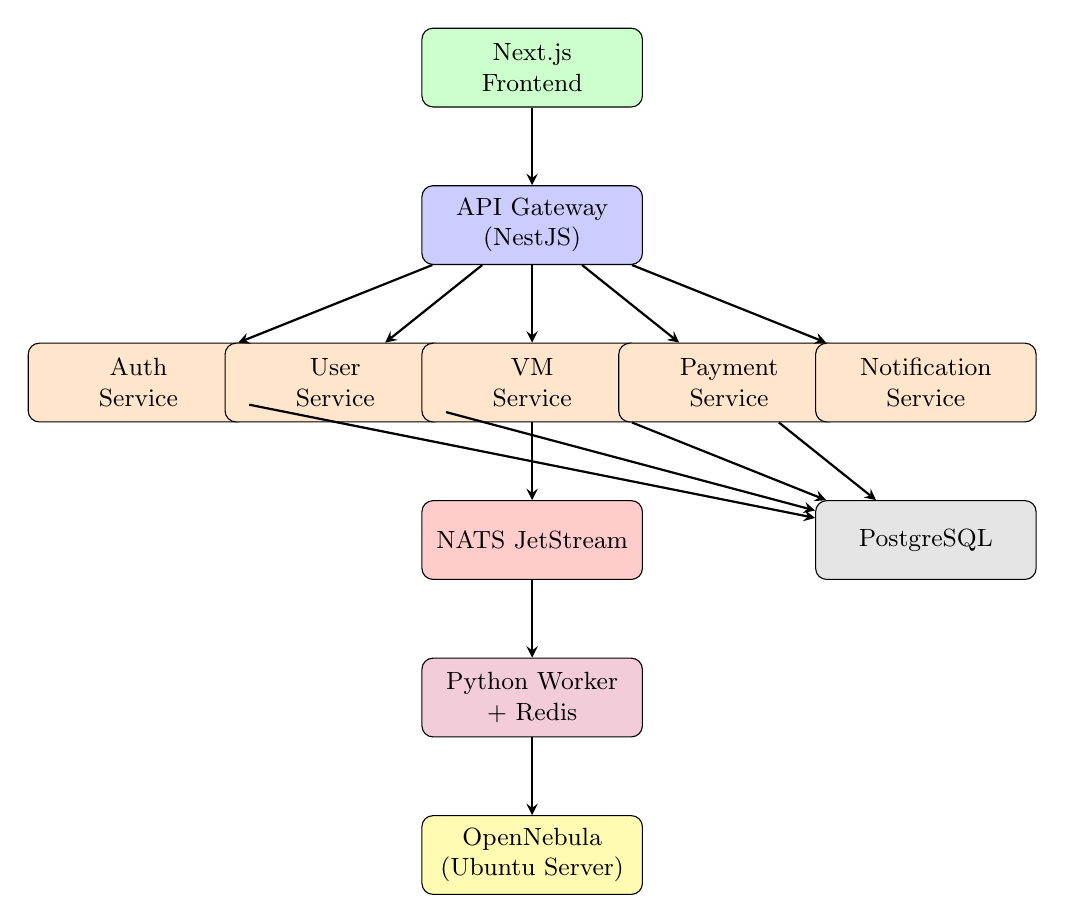
\begin{tikzpicture}[
  box/.style={draw, rounded corners, minimum width=2.8cm, minimum height=1cm, align=center, font=\small},
  arrow/.style={->, thick, >=stealth}
]
  % Frontend
  \node[box, fill=green!20] (frontend) at (0, 4) {Next.js\\Frontend};
  
  % API Gateway
  \node[box, fill=blue!20] (gateway) at (0, 2) {API Gateway\\(NestJS)};
  
  % Services
  \node[box, fill=orange!20] (auth) at (-5, 0) {Auth\\Service};
  \node[box, fill=orange!20] (user) at (-2.5, 0) {User\\Service};
  \node[box, fill=orange!20] (vm) at (0, 0) {VM\\Service};
  \node[box, fill=orange!20] (payment) at (2.5, 0) {Payment\\Service};
  \node[box, fill=orange!20] (notif) at (5, 0) {Notification\\Service};
  
  % Message Queue
  \node[box, fill=red!20] (nats) at (0, -2) {NATS JetStream};
  
  % Worker
  \node[box, fill=purple!20] (worker) at (0, -4) {Python Worker\\+ Redis};
  
  % OpenNebula
  \node[box, fill=yellow!30] (opennebula) at (0, -6) {OpenNebula\\(Ubuntu Server)};
  
  % Database
  \node[box, fill=gray!20] (db) at (5, -2) {PostgreSQL};
  
  % Arrows
  \draw[arrow] (frontend) -- (gateway);
  \draw[arrow] (gateway) -- (auth);
  \draw[arrow] (gateway) -- (user);
  \draw[arrow] (gateway) -- (vm);
  \draw[arrow] (gateway) -- (payment);
  \draw[arrow] (gateway) -- (notif);
  \draw[arrow] (vm) -- (nats);
  \draw[arrow] (nats) -- (worker);
  \draw[arrow] (worker) -- (opennebula);
  \draw[arrow] (auth) -- (db);
  \draw[arrow] (user) -- (db);
  \draw[arrow] (vm) -- (db);
  \draw[arrow] (payment) -- (db);
  
\end{tikzpicture}
\caption{Global architecture of the CloudVM platform}
\label{fig:architecture}
\end{figure}

% ============================================================
\section{Methodology}

\subsection{Choice of Methodology}

For this project, we adopted the \textbf{Agile methodology} with the \textbf{Scrum framework}. This choice was motivated by several factors:

\begin{itemize}
  \item \textbf{Iterative development:} Allows delivering working features incrementally.
  \item \textbf{Flexibility:} Adapts to changing requirements during the project.
  \item \textbf{Regular feedback:} Checkpoints at the end of each sprint ensure quality.
  \item \textbf{Team collaboration:} Clear roles and daily coordination between DSI and RSI students.
\end{itemize}

\subsection{Scrum Roles}

\begin{table}[H]
\centering
\caption{Scrum roles in the project}
\label{tab:scrum-roles}
\begin{tabularx}{\textwidth}{|l|X|}
\hline
\rowcolor{blue!15}
\textbf{Role} & \textbf{Assigned To} \\
\hline
Product Owner & Project Supervisor \\
\hline
Scrum Master & DSI Student \\
\hline
Development Team & DSI Student (Web Development) + RSI Student (Infrastructure) \\
\hline
\end{tabularx}
\end{table}

\subsection{Sprint Organization}

The project is organized into \textbf{8 sprints}, each lasting \textbf{one week}. Each sprint follows the standard Scrum cycle:

\begin{enumerate}
  \item \textbf{Sprint Planning:} Define sprint goal and select user stories from the backlog.
  \item \textbf{Daily Work:} Implement tasks according to the sprint backlog.
  \item \textbf{Sprint Review:} Demonstrate completed features (checkpoint).
  \item \textbf{Sprint Retrospective:} Reflect on the process and improve.
\end{enumerate}

\begin{figure}[H]
\centering
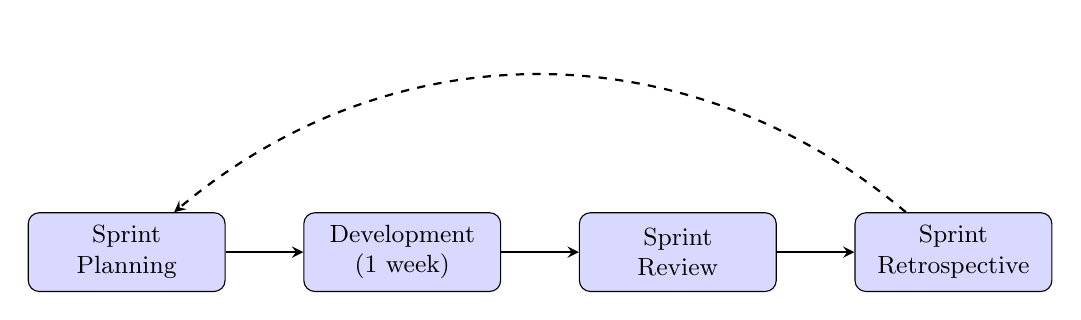
\begin{tikzpicture}[
  box/.style={draw, rounded corners, minimum width=2.5cm, minimum height=1cm, align=center, font=\small, fill=blue!15},
  arrow/.style={->, thick, >=stealth}
]
  \node[box] (plan) at (0, 0) {Sprint\\Planning};
  \node[box] (dev) at (3.5, 0) {Development\\(1 week)};
  \node[box] (review) at (7, 0) {Sprint\\Review};
  \node[box] (retro) at (10.5, 0) {Sprint\\Retrospective};
  
  \draw[arrow] (plan) -- (dev);
  \draw[arrow] (dev) -- (review);
  \draw[arrow] (review) -- (retro);
  \draw[arrow, dashed] (retro) to[bend right=40] (plan);
\end{tikzpicture}
\caption{Scrum sprint cycle}
\label{fig:scrum-cycle}
\end{figure}

\subsection{Sprint Planning Overview}

\begin{table}[H]
\centering
\caption{Sprint planning overview}
\label{tab:sprint-plan}
\begin{tabularx}{\textwidth}{|c|l|X|}
\hline
\rowcolor{blue!15}
\textbf{Sprint} & \textbf{Week} & \textbf{Goal} \\
\hline
Sprint 1 & Week 1 & Project foundation + Landing page \\
\hline
Sprint 2 & Week 2 & Authentication service (register, login, JWT) \\
\hline
Sprint 3 & Week 3 & User management + Dashboard layout + Firewall \\
\hline
Sprint 4 & Week 4 & VM management (create, start, stop, delete) + Worker \\
\hline
Sprint 5 & Week 5 & VM dashboard + Quota system \\
\hline
Sprint 6 & Week 6 & Payment service + Plan management \\
\hline
Sprint 7 & Week 7 & Notifications + Integration testing + Polish \\
\hline
Sprint 8 & Week 8 & Deployment + Documentation + Presentation \\
\hline
\end{tabularx}
\end{table}

% ============================================================
\section{Product Backlog}

The product backlog contains all user stories prioritized by business value. Each user story follows the standard format: \textit{``As a [role], I want to [action] so that [benefit].''}

\subsection{Actors Identification}

The system identifies three main actors:

\begin{itemize}
  \item \textbf{Visitor:} An unauthenticated user who can only view the landing page and pricing.
  \item \textbf{User:} An authenticated user who can manage virtual machines within their quota.
  \item \textbf{Administrator:} A platform administrator who can manage users, VMs, and plans.
\end{itemize}

\subsection{Global Use Case Diagram}

\begin{figure}[H]
\centering
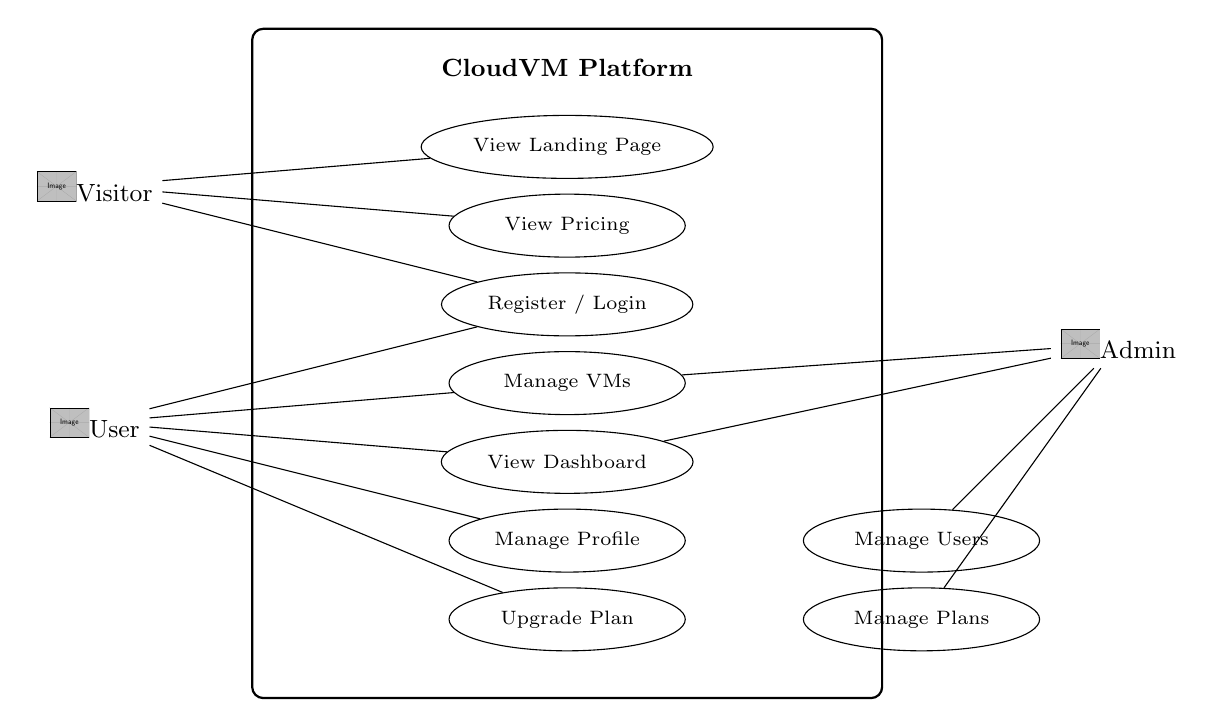
\begin{tikzpicture}[
  actor/.style={font=\small},
  usecase/.style={draw, ellipse, minimum width=3cm, minimum height=0.8cm, align=center, font=\scriptsize},
  arrow/.style={->, thick, >=stealth}
]
  % System boundary
  \draw[thick, rounded corners] (-1, -7.5) rectangle (7, 1);
  \node[font=\small\bfseries] at (3, 0.5) {CloudVM Platform};
  
  % Actors
  \node[actor] (visitor) at (-3, -1) {\includegraphics[width=0.5cm]{example-image}\\Visitor};
  \node[actor] (user) at (-3, -4) {\includegraphics[width=0.5cm]{example-image}\\User};
  \node[actor] (admin) at (10, -3) {\includegraphics[width=0.5cm]{example-image}\\Admin};
  
  % Use cases - Visitor
  \node[usecase] (uc1) at (3, -0.5) {View Landing Page};
  \node[usecase] (uc2) at (3, -1.5) {View Pricing};
  \node[usecase] (uc3) at (3, -2.5) {Register / Login};
  
  % Use cases - User
  \node[usecase] (uc4) at (3, -3.5) {Manage VMs};
  \node[usecase] (uc5) at (3, -4.5) {View Dashboard};
  \node[usecase] (uc6) at (3, -5.5) {Manage Profile};
  \node[usecase] (uc7) at (3, -6.5) {Upgrade Plan};
  
  % Arrows - Visitor
  \draw (visitor) -- (uc1);
  \draw (visitor) -- (uc2);
  \draw (visitor) -- (uc3);
  
  % Arrows - User
  \draw (user) -- (uc3);
  \draw (user) -- (uc4);
  \draw (user) -- (uc5);
  \draw (user) -- (uc6);
  \draw (user) -- (uc7);
  
  % Arrows - Admin
  \draw (admin) -- (uc4);
  \draw (admin) -- (uc5);
  \node[usecase] (uc8) at (7.5, -5.5) {Manage Users};
  \node[usecase] (uc9) at (7.5, -6.5) {Manage Plans};
  \draw (admin) -- (uc8);
  \draw (admin) -- (uc9);
  
\end{tikzpicture}
\caption{Global use case diagram}
\label{fig:global-usecase}
\end{figure}

\subsection{User Stories}

The following tables present the complete product backlog organized by epics.

\subsubsection{Epic 1: Authentication \& User Management}

\begin{longtable}{|c|p{7cm}|c|c|}
\hline
\rowcolor{blue!15}
\textbf{ID} & \textbf{User Story} & \textbf{Priority} & \textbf{Sprint} \\
\hline
\endhead
US-01 & As a visitor, I want to register an account so that I can access the platform. & High & 2 \\
\hline
US-02 & As a visitor, I want to log in with my credentials so that I can access my dashboard. & High & 2 \\
\hline
US-03 & As a user, I want to log out securely so that my session is terminated. & High & 2 \\
\hline
US-04 & As a user, I want to reset my password so that I can recover my account. & Medium & 2 \\
\hline
US-05 & As an admin, I want to view all users so that I can manage the platform. & High & 3 \\
\hline
US-06 & As an admin, I want to delete/ban a user so that I can moderate the platform. & High & 3 \\
\hline
US-07 & As a user, I want to update my profile so that my information is current. & Medium & 3 \\
\hline
\caption{User stories — Authentication \& User Management}
\label{tab:us-auth}
\end{longtable}

\subsubsection{Epic 2: Landing Page \& UI}

\begin{longtable}{|c|p{7cm}|c|c|}
\hline
\rowcolor{blue!15}
\textbf{ID} & \textbf{User Story} & \textbf{Priority} & \textbf{Sprint} \\
\hline
\endhead
US-08 & As a visitor, I want to see a landing page so that I understand what the platform offers. & High & 1 \\
\hline
US-09 & As a visitor, I want to see pricing plans so that I can choose a plan. & High & 1 \\
\hline
US-10 & As a user, I want a responsive dashboard so that I can manage my VMs easily. & High & 3 \\
\hline
\caption{User stories — Landing Page \& UI}
\label{tab:us-ui}
\end{longtable}

\subsubsection{Epic 3: VM Management}

\begin{longtable}{|c|p{7cm}|c|c|}
\hline
\rowcolor{blue!15}
\textbf{ID} & \textbf{User Story} & \textbf{Priority} & \textbf{Sprint} \\
\hline
\endhead
US-11 & As a user, I want to create a VM so that I can use cloud resources. & High & 4 \\
\hline
US-12 & As a user, I want to start a stopped VM so that I can resume work. & High & 4 \\
\hline
US-13 & As a user, I want to stop a running VM so that I can save resources. & High & 4 \\
\hline
US-14 & As a user, I want to reboot a VM so that I can fix issues. & High & 4 \\
\hline
US-15 & As a user, I want to delete a VM so that I free my quota. & High & 4 \\
\hline
US-16 & As a user, I want to see VM details (IP, status, resources) so that I can monitor usage. & High & 5 \\
\hline
US-17 & As a user, I want to see all my VMs in a list so that I can manage them. & High & 4 \\
\hline
US-18 & As an admin, I want to manage all VMs so that I can oversee the platform. & High & 5 \\
\hline
US-19 & As a user, I want to be notified of VM status changes so that I stay informed. & Medium & 7 \\
\hline
US-29 & As a user, I want to manage SSH keys so that I can securely connect to my VMs. & High & 3 \\
\hline
US-30 & As a user, I want to access a web terminal (CLI) for my VM so that I can use it from the browser. & High & 5 \\
\hline
\caption{User stories — VM Management}
\label{tab:us-vm}
\end{longtable}

\subsubsection{Epic 4: Payment \& Quota Management}

\begin{longtable}{|c|p{7cm}|c|c|}
\hline
\rowcolor{blue!15}
\textbf{ID} & \textbf{User Story} & \textbf{Priority} & \textbf{Sprint} \\
\hline
\endhead
US-20 & As a user, I want to see my current quota so that I know my limits. & High & 5 \\
\hline
US-21 & As a user, I want to upgrade my plan so that I get more resources. & High & 6 \\
\hline
US-22 & As a user, I want to see payment history so that I can track expenses. & Medium & 6 \\
\hline
US-23 & As an admin, I want to manage pricing plans so that the business model is flexible. & High & 6 \\
\hline
US-24 & As a user, I want the system to block VM creation when quota is exceeded so that limits are enforced. & High & 5 \\
\hline
\caption{User stories — Payment \& Quota Management}
\label{tab:us-payment}
\end{longtable}

\subsubsection{Epic 5: Infrastructure \& Security (RSI)}

\begin{longtable}{|c|p{7cm}|c|c|}
\hline
\rowcolor{blue!15}
\textbf{ID} & \textbf{User Story} & \textbf{Priority} & \textbf{Sprint} \\
\hline
\endhead
US-25 & As an operator, I want OpenNebula installed and configured so that VMs can be provisioned. & High & 2--3 \\
\hline
US-26 & As an operator, I want firewall rules configured so that the server is secure. & High & 3 \\
\hline
US-27 & As an operator, I want the server monitored so that I can detect issues. & Medium & 6 \\
\hline
US-28 & As an operator, I want the API server to communicate with OpenNebula so that VM operations work. & High & 4 \\
\hline
\caption{User stories — Infrastructure \& Security}
\label{tab:us-infra}
\end{longtable}

% ============================================================
\section{Development Environment and Tools}

This section presents the hardware and software tools used for developing the CloudVM platform.

\subsection{Hardware Environment}

\begin{table}[H]
\centering
\caption{Hardware environment}
\label{tab:hardware}
\begin{tabularx}{\textwidth}{|l|X|}
\hline
\rowcolor{blue!15}
\textbf{Component} & \textbf{Description} \\
\hline
Development Machine & Personal laptop (DSI Student) \\
\hline
Server Machine & Dedicated machine running Ubuntu Server 22.04/24.04 LTS (RSI Student) \\
\hline
Network & Local network for development, SSH access to server \\
\hline
\end{tabularx}
\end{table}

\subsection{Software Environment}

\subsubsection{Frontend Technologies}

\begin{table}[H]
\centering
\caption{Frontend technologies}
\label{tab:frontend-tech}
\begin{tabularx}{\textwidth}{|l|l|X|}
\hline
\rowcolor{blue!15}
\textbf{Technology} & \textbf{Version} & \textbf{Purpose} \\
\hline
Next.js & 14+ & React-based framework with server-side rendering and App Router \\
\hline
Tailwind CSS & 3.x & Utility-first CSS framework for responsive design \\
\hline
TypeScript & 5.x & Type-safe JavaScript for frontend development \\
\hline
React Query & 5.x & Server state management and API caching \\
\hline
xterm.js & 5.x & Terminal emulator for web-based CLI access to VMs (Phase~1) \\
\hline
Socket.IO & 4.x & WebSocket library for real-time terminal communication \\
\hline
\end{tabularx}
\end{table}

\subsubsection{Backend Technologies}

\begin{table}[H]
\centering
\caption{Backend technologies}
\label{tab:backend-tech}
\begin{tabularx}{\textwidth}{|l|l|X|}
\hline
\rowcolor{blue!15}
\textbf{Technology} & \textbf{Version} & \textbf{Purpose} \\
\hline
NestJS & 10.x & Progressive Node.js framework for microservices \\
\hline
TypeScript & 5.x & Type-safe backend development \\
\hline
Prisma & 5.x & ORM for database access and migrations \\
\hline
PostgreSQL & 16 & Relational database for persistent data storage \\
\hline
JWT & — & JSON Web Tokens for stateless authentication \\
\hline
bcrypt & — & Password hashing library \\
\hline
ssh2 & — & SSH client library for Node.js (WebSocket-to-SSH proxy for web terminal) \\
\hline
\end{tabularx}
\end{table}

\subsubsection{Worker \& Message Queue}

\begin{table}[H]
\centering
\caption{Worker and message queue technologies}
\label{tab:worker-tech}
\begin{tabularx}{\textwidth}{|l|l|X|}
\hline
\rowcolor{blue!15}
\textbf{Technology} & \textbf{Version} & \textbf{Purpose} \\
\hline
Python & 3.11+ & Worker process for async VM operations \\
\hline
NATS JetStream & Latest & Persistent message queue for service communication \\
\hline
Redis & 7.x & Caching and task state management \\
\hline
pyone & Latest & Python bindings for OpenNebula XML-RPC API \\
\hline
\end{tabularx}
\end{table}

\subsubsection{Infrastructure Technologies}

\begin{table}[H]
\centering
\caption{Infrastructure technologies}
\label{tab:infra-tech}
\begin{tabularx}{\textwidth}{|l|l|X|}
\hline
\rowcolor{blue!15}
\textbf{Technology} & \textbf{Version} & \textbf{Purpose} \\
\hline
Ubuntu Server & 22.04/24.04 LTS & Server operating system \\
\hline
OpenNebula & 6.x & Cloud computing platform for VM orchestration \\
\hline
KVM & Latest & Hypervisor for hardware-level virtualization \\
\hline
iptables/nftables & — & Firewall for network security \\
\hline
Docker & 24.x & Container runtime for service isolation \\
\hline
Docker Compose & 2.x & Multi-container orchestration \\
\hline
\end{tabularx}
\end{table}

\subsubsection{Development Tools}

\begin{table}[H]
\centering
\caption{Development tools}
\label{tab:dev-tools}
\begin{tabularx}{\textwidth}{|l|X|}
\hline
\rowcolor{blue!15}
\textbf{Tool} & \textbf{Purpose} \\
\hline
Visual Studio Code & Primary code editor with extensions \\
\hline
Figma & UI/UX design and prototyping \\
\hline
Git + GitHub/GitLab & Version control and code hosting \\
\hline
Postman & API development and testing \\
\hline
Docker Desktop & Local container management \\
\hline
\LaTeX{} (Overleaf) & Report writing \\
\hline
Draw.io / Lucidchart & Diagram creation (UML, architecture) \\
\hline
\end{tabularx}
\end{table}

% ============================================================
\section{Conclusion}

In this chapter, we presented the general context of our project. We introduced the host organization Readdly, analyzed existing cloud VM platforms, and identified their limitations. Our proposed solution, CloudVM, addresses these gaps by offering a self-hosted, open-source platform with a modern microservices architecture.

We also presented our development methodology (Agile/Scrum), defined the complete product backlog with 28 user stories organized into 5 epics, and detailed the development environment and tools that will be used throughout the project.

In the next chapter, we will begin the implementation phase with Sprint 1 (Landing Page) and Sprint 2 (Authentication Service).


% ============================================================
% CHAPTER 2: Sprint 1 & 2 (Landing Page + Auth)
% ============================================================
% % ============================================================
% CHAPTER 2: Sprint 1 & Sprint 2 — Landing Page + Authentication
% ============================================================
% ADD THIS TO main.tex AFTER COMPLETING SPRINT 1 & 2
% Uncomment: % ============================================================
% CHAPTER 2: Sprint 1 & Sprint 2 — Landing Page + Authentication
% ============================================================
% ADD THIS TO main.tex AFTER COMPLETING SPRINT 1 & 2
% Uncomment: % ============================================================
% CHAPTER 2: Sprint 1 & Sprint 2 — Landing Page + Authentication
% ============================================================
% ADD THIS TO main.tex AFTER COMPLETING SPRINT 1 & 2
% Uncomment: \input{chapters/chapter2}
% ============================================================
\chapter{Sprint 1 \& Sprint 2: Foundation and Authentication}

\section{Introduction}

This chapter covers the first two sprints of the project. Sprint 1 focuses on establishing the project foundation and building the landing page, while Sprint 2 implements the authentication service with JWT-based security.

% ============================================================
% SPRINT 1
% ============================================================
\section{Sprint 1: Landing Page \& Project Foundation}

\sprintcard{1}{Landing Page \& Project Foundation}{Deliver a responsive landing page and set up the project skeleton with Docker containers.}

\subsection{Sprint Backlog}

\begin{longtable}{|c|p{5cm}|c|c|c|}
\hline
\rowcolor{blue!15}
\textbf{Task ID} & \textbf{Task} & \textbf{Assignee} & \textbf{Est.} & \textbf{Status} \\
\hline
\endhead
T-1.1 & Scaffold Next.js project & DSI & 2h & Done \\
\hline
T-1.2 & Scaffold NestJS microservices & DSI & 4h & Done \\
\hline
T-1.3 & Setup Docker Compose & DSI & 3h & Done \\
\hline
T-1.4 & Setup PostgreSQL + ORM & DSI & 3h & Done \\
\hline
T-1.5 & Landing page — Hero section & DSI & 4h & Done \\
\hline
T-1.6 & Landing page — Pricing section & DSI & 4h & Done \\
\hline
T-1.7 & Landing page — Features + Footer & DSI & 3h & Done \\
\hline
T-1.8 & Responsive design + Polish & DSI & 4h & Done \\
\hline
T-1.9 & Ubuntu Server hardening & RSI & 4h & Done \\
\hline
T-1.10 & Network configuration & RSI & 3h & Done \\
\hline
T-1.11 & Docker install on server & RSI & 2h & Done \\
\hline
T-1.12 & OpenNebula research & RSI & 6h & Done \\
\hline
\caption{Sprint 1 backlog}
\label{tab:sprint1-backlog}
\end{longtable}

\subsection{Mockups and Design}

% INSERT FIGMA SCREENSHOTS HERE
\begin{figure}[H]
\centering
% \includegraphics[width=\textwidth]{images/landing-mockup.png}
\fbox{\parbox{0.9\textwidth}{\centering\vspace{3cm}\textit{Insert Figma landing page mockup here}\vspace{3cm}}}
\caption{Landing page mockup (Figma)}
\label{fig:landing-mockup}
\end{figure}

\subsection{Implementation}

\subsubsection{Project Structure}

The project follows a monorepo structure with separate directories for each microservice:

\begin{lstlisting}[language=bash, caption={Project directory structure}]
cloudvm/
├── frontend/          # Next.js application
├── services/
│   ├── gateway/       # API Gateway (NestJS)
│   ├── auth/          # Auth Service (NestJS)
│   ├── user/          # User Service (NestJS)
│   ├── vm/            # VM Service (NestJS)
│   └── payment/       # Payment Service (NestJS)
├── worker/            # Python Worker
├── docker-compose.yml
└── .env
\end{lstlisting}

\subsubsection{Landing Page Screenshots}

% INSERT ACTUAL SCREENSHOTS HERE
\begin{figure}[H]
\centering
\fbox{\parbox{0.9\textwidth}{\centering\vspace{3cm}\textit{Insert landing page hero section screenshot}\vspace{3cm}}}
\caption{Landing page — Hero section}
\label{fig:landing-hero}
\end{figure}

\begin{figure}[H]
\centering
\fbox{\parbox{0.9\textwidth}{\centering\vspace{3cm}\textit{Insert landing page pricing section screenshot}\vspace{3cm}}}
\caption{Landing page — Pricing section}
\label{fig:landing-pricing}
\end{figure}

\subsection{Sprint 1 Review}

At the end of Sprint 1, the following deliverables were achieved:
\begin{itemize}
  \item Responsive landing page with hero, features, pricing, and footer sections.
  \item Docker Compose configuration with containers for all microservices.
  \item PostgreSQL database initialized with ORM configuration.
  \item Ubuntu Server hardened with SSH key authentication.
  \item Docker installed and configured on the server.
\end{itemize}


% ============================================================
% SPRINT 2
% ============================================================
\section{Sprint 2: Authentication Service}

\sprintcard{2}{Authentication Service}{Implement secure user registration, login, JWT authentication, and role-based access control.}

\subsection{Sprint Backlog}

\begin{longtable}{|c|p{5cm}|c|c|c|}
\hline
\rowcolor{blue!15}
\textbf{Task ID} & \textbf{Task} & \textbf{Assignee} & \textbf{Est.} & \textbf{Status} \\
\hline
\endhead
T-2.1 & Registration endpoint & DSI & 4h & Done \\
\hline
T-2.2 & Login endpoint & DSI & 4h & Done \\
\hline
T-2.3 & JWT + Refresh tokens & DSI & 4h & Done \\
\hline
T-2.4 & Logout + token blacklist & DSI & 2h & Done \\
\hline
T-2.5 & Password reset flow & DSI & 3h & Done \\
\hline
T-2.6 & Auth guards (JWT, Role) & DSI & 3h & Done \\
\hline
T-2.7 & Register page (frontend) & DSI & 4h & Done \\
\hline
T-2.8 & Login page (frontend) & DSI & 3h & Done \\
\hline
T-2.9 & Auth state management & DSI & 3h & Done \\
\hline
T-2.10 & OpenNebula installation & RSI & 6h & Done \\
\hline
T-2.11 & OpenNebula configuration & RSI & 6h & Done \\
\hline
T-2.12 & KVM setup + VM templates & RSI & 6h & Done \\
\hline
\caption{Sprint 2 backlog}
\label{tab:sprint2-backlog}
\end{longtable}

\subsection{Use Case Diagram — Authentication}

\begin{figure}[H]
\centering
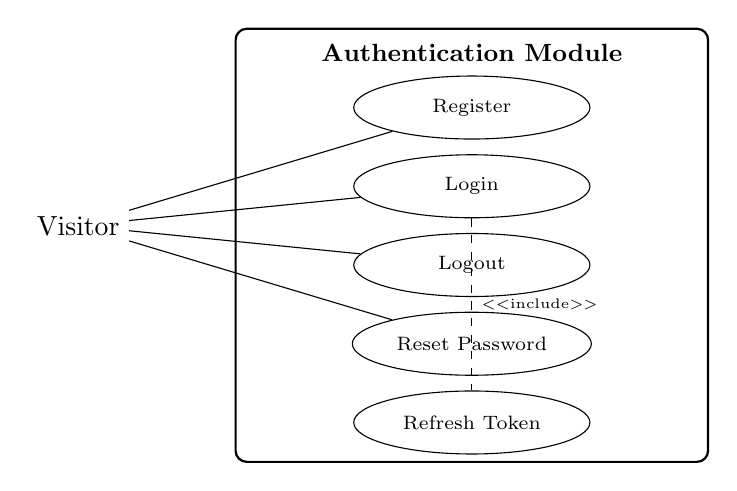
\begin{tikzpicture}[
  usecase/.style={draw, ellipse, minimum width=3cm, minimum height=0.8cm, align=center, font=\scriptsize}
]
  % System boundary
  \draw[thick, rounded corners] (0, -5) rectangle (6, 0.5);
  \node[font=\small\bfseries] at (3, 0.2) {Authentication Module};
  
  % Actor
  \node (visitor) at (-2, -2) {Visitor};
  
  % Use cases
  \node[usecase] (uc1) at (3, -0.5) {Register};
  \node[usecase] (uc2) at (3, -1.5) {Login};
  \node[usecase] (uc3) at (3, -2.5) {Logout};
  \node[usecase] (uc4) at (3, -3.5) {Reset Password};
  \node[usecase] (uc5) at (3, -4.5) {Refresh Token};
  
  % Arrows
  \draw (visitor) -- (uc1);
  \draw (visitor) -- (uc2);
  \draw (visitor) -- (uc3);
  \draw (visitor) -- (uc4);
  \draw[dashed] (uc2) -- node[right, font=\tiny] {<<include>>} (uc5);
  
\end{tikzpicture}
\caption{Use case diagram — Authentication}
\label{fig:uc-auth}
\end{figure}

\subsection{Sequence Diagram — Registration}

\begin{figure}[H]
\centering
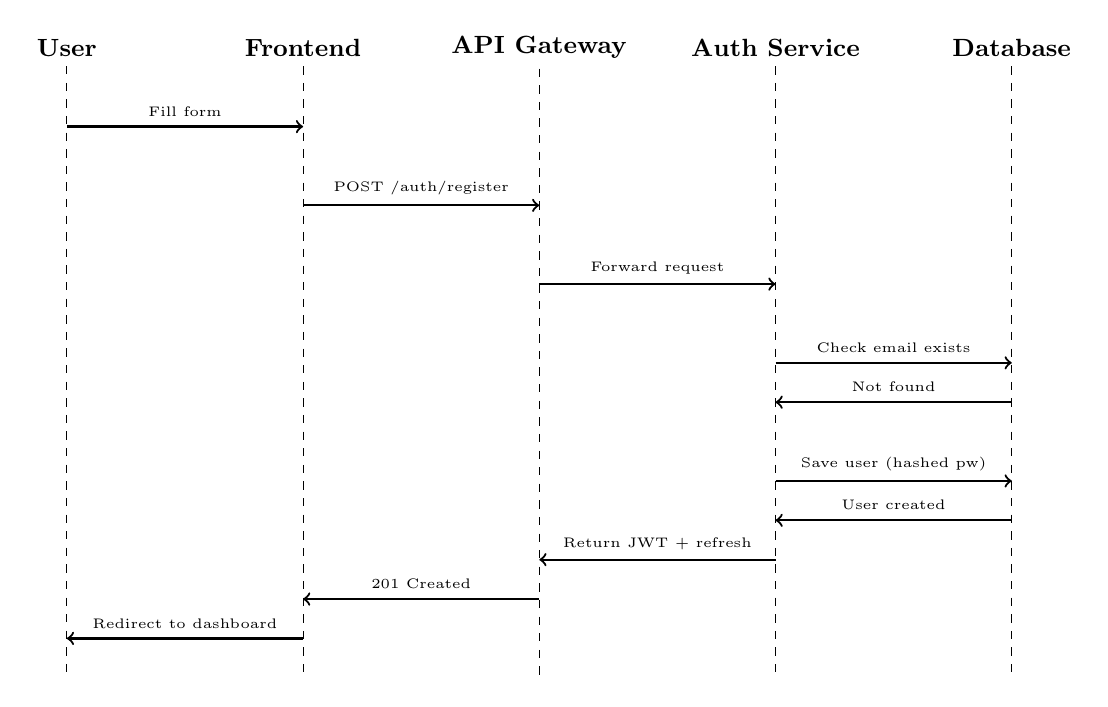
\begin{tikzpicture}[font=\small]
  % Lifelines
  \node (user) at (0, 0) {\textbf{User}};
  \node (front) at (3, 0) {\textbf{Frontend}};
  \node (gate) at (6, 0) {\textbf{API Gateway}};
  \node (auth) at (9, 0) {\textbf{Auth Service}};
  \node (db) at (12, 0) {\textbf{Database}};
  
  \draw[dashed] (user) -- (0, -8);
  \draw[dashed] (front) -- (3, -8);
  \draw[dashed] (gate) -- (6, -8);
  \draw[dashed] (auth) -- (9, -8);
  \draw[dashed] (db) -- (12, -8);
  
  % Messages
  \draw[->, thick] (0, -1) -- node[above, font=\tiny] {Fill form} (3, -1);
  \draw[->, thick] (3, -2) -- node[above, font=\tiny] {POST /auth/register} (6, -2);
  \draw[->, thick] (6, -3) -- node[above, font=\tiny] {Forward request} (9, -3);
  \draw[->, thick] (9, -4) -- node[above, font=\tiny] {Check email exists} (12, -4);
  \draw[<-, thick] (9, -4.5) -- node[above, font=\tiny] {Not found} (12, -4.5);
  \draw[->, thick] (9, -5.5) -- node[above, font=\tiny] {Save user (hashed pw)} (12, -5.5);
  \draw[<-, thick] (9, -6) -- node[above, font=\tiny] {User created} (12, -6);
  \draw[<-, thick] (6, -6.5) -- node[above, font=\tiny] {Return JWT + refresh} (9, -6.5);
  \draw[<-, thick] (3, -7) -- node[above, font=\tiny] {201 Created} (6, -7);
  \draw[<-, thick] (0, -7.5) -- node[above, font=\tiny] {Redirect to dashboard} (3, -7.5);
\end{tikzpicture}
\caption{Sequence diagram — User registration}
\label{fig:seq-register}
\end{figure}

\subsection{Sequence Diagram — Login}

\begin{figure}[H]
\centering
\begin{tikzpicture}[font=\small]
  % Lifelines
  \node (user) at (0, 0) {\textbf{User}};
  \node (front) at (3, 0) {\textbf{Frontend}};
  \node (gate) at (6, 0) {\textbf{API Gateway}};
  \node (auth) at (9, 0) {\textbf{Auth Service}};
  \node (db) at (12, 0) {\textbf{Database}};
  
  \draw[dashed] (user) -- (0, -8);
  \draw[dashed] (front) -- (3, -8);
  \draw[dashed] (gate) -- (6, -8);
  \draw[dashed] (auth) -- (9, -8);
  \draw[dashed] (db) -- (12, -8);
  
  % Messages
  \draw[->, thick] (0, -1) -- node[above, font=\tiny] {Enter credentials} (3, -1);
  \draw[->, thick] (3, -2) -- node[above, font=\tiny] {POST /auth/login} (6, -2);
  \draw[->, thick] (6, -3) -- node[above, font=\tiny] {Forward request} (9, -3);
  \draw[->, thick] (9, -4) -- node[above, font=\tiny] {Find user by email} (12, -4);
  \draw[<-, thick] (9, -4.5) -- node[above, font=\tiny] {User found} (12, -4.5);
  \draw[->, thick] (9, -5) -- node[right, font=\tiny] {Compare passwords};
  \draw[->, thick] (9, -5.5) -- node[right, font=\tiny] {Generate JWT + refresh};
  \draw[<-, thick] (6, -6) -- node[above, font=\tiny] {Return tokens} (9, -6);
  \draw[<-, thick] (3, -6.5) -- node[above, font=\tiny] {200 OK + tokens} (6, -6.5);
  \draw[<-, thick] (0, -7) -- node[above, font=\tiny] {Store token, redirect} (3, -7);
\end{tikzpicture}
\caption{Sequence diagram — User login}
\label{fig:seq-login}
\end{figure}

\subsection{Class Diagram — Auth Module}

\begin{figure}[H]
\centering
\begin{tikzpicture}[font=\small,
  class/.style={draw, rectangle, minimum width=4cm, align=left}
]
  % User class
  \node[class, fill=yellow!15] (userclass) at (0, 0) {
    \textbf{User}\\
    \hline
    - id: UUID\\
    - email: String\\
    - password: String\\
    - firstName: String\\
    - lastName: String\\
    - role: Role\\
    - createdAt: DateTime\\
    - updatedAt: DateTime\\
    \hline
    + register()\\
    + login()\\
    + resetPassword()
  };
  
  % Role enum
  \node[class, fill=green!15] (roleenum) at (6, 0) {
    \textbf{<<enum>> Role}\\
    \hline
    USER\\
    ADMIN
  };
  
  % RefreshToken class
  \node[class, fill=blue!15] (tokenclass) at (0, -5.5) {
    \textbf{RefreshToken}\\
    \hline
    - id: UUID\\
    - token: String\\
    - userId: UUID\\
    - expiresAt: DateTime\\
    - isRevoked: Boolean\\
    \hline
    + revoke()
  };
  
  % Relations
  \draw[->, thick] (userclass) -- node[above, font=\tiny] {has} (roleenum);
  \draw[->, thick] (userclass) -- node[left, font=\tiny] {has many} (tokenclass);
\end{tikzpicture}
\caption{Class diagram — Authentication module}
\label{fig:class-auth}
\end{figure}

\subsection{Implementation Screenshots}

% INSERT ACTUAL SCREENSHOTS HERE
\begin{figure}[H]
\centering
\fbox{\parbox{0.9\textwidth}{\centering\vspace{3cm}\textit{Insert registration page screenshot}\vspace{3cm}}}
\caption{Registration page}
\label{fig:register-page}
\end{figure}

\begin{figure}[H]
\centering
\fbox{\parbox{0.9\textwidth}{\centering\vspace{3cm}\textit{Insert login page screenshot}\vspace{3cm}}}
\caption{Login page}
\label{fig:login-page}
\end{figure}

\subsection{Sprint 2 Review}

At the end of Sprint 2, the following deliverables were achieved:
\begin{itemize}
  \item Complete auth service with registration, login, logout, password reset.
  \item JWT + refresh token implementation with role-based guards.
  \item Login and registration pages with form validation.
  \item OpenNebula installed and configured on the server.
  \item KVM hypervisor operational with VM templates.
\end{itemize}

% ============================================================
\section{Conclusion}

In this chapter, we completed the first two sprints. Sprint 1 established the project foundation with a modern landing page and Docker-based development environment. Sprint 2 delivered a complete authentication system with secure JWT-based access control. On the infrastructure side, OpenNebula was installed and configured for VM provisioning.

In the next chapter, we will cover Sprint 3 (User Management \& Dashboard) and Sprint 4 (VM Management \& Worker Service).

% ============================================================
\chapter{Sprint 1 \& Sprint 2: Foundation and Authentication}

\section{Introduction}

This chapter covers the first two sprints of the project. Sprint 1 focuses on establishing the project foundation and building the landing page, while Sprint 2 implements the authentication service with JWT-based security.

% ============================================================
% SPRINT 1
% ============================================================
\section{Sprint 1: Landing Page \& Project Foundation}

\sprintcard{1}{Landing Page \& Project Foundation}{Deliver a responsive landing page and set up the project skeleton with Docker containers.}

\subsection{Sprint Backlog}

\begin{longtable}{|c|p{5cm}|c|c|c|}
\hline
\rowcolor{blue!15}
\textbf{Task ID} & \textbf{Task} & \textbf{Assignee} & \textbf{Est.} & \textbf{Status} \\
\hline
\endhead
T-1.1 & Scaffold Next.js project & DSI & 2h & Done \\
\hline
T-1.2 & Scaffold NestJS microservices & DSI & 4h & Done \\
\hline
T-1.3 & Setup Docker Compose & DSI & 3h & Done \\
\hline
T-1.4 & Setup PostgreSQL + ORM & DSI & 3h & Done \\
\hline
T-1.5 & Landing page — Hero section & DSI & 4h & Done \\
\hline
T-1.6 & Landing page — Pricing section & DSI & 4h & Done \\
\hline
T-1.7 & Landing page — Features + Footer & DSI & 3h & Done \\
\hline
T-1.8 & Responsive design + Polish & DSI & 4h & Done \\
\hline
T-1.9 & Ubuntu Server hardening & RSI & 4h & Done \\
\hline
T-1.10 & Network configuration & RSI & 3h & Done \\
\hline
T-1.11 & Docker install on server & RSI & 2h & Done \\
\hline
T-1.12 & OpenNebula research & RSI & 6h & Done \\
\hline
\caption{Sprint 1 backlog}
\label{tab:sprint1-backlog}
\end{longtable}

\subsection{Mockups and Design}

% INSERT FIGMA SCREENSHOTS HERE
\begin{figure}[H]
\centering
% \includegraphics[width=\textwidth]{images/landing-mockup.png}
\fbox{\parbox{0.9\textwidth}{\centering\vspace{3cm}\textit{Insert Figma landing page mockup here}\vspace{3cm}}}
\caption{Landing page mockup (Figma)}
\label{fig:landing-mockup}
\end{figure}

\subsection{Implementation}

\subsubsection{Project Structure}

The project follows a monorepo structure with separate directories for each microservice:

\begin{lstlisting}[language=bash, caption={Project directory structure}]
cloudvm/
├── frontend/          # Next.js application
├── services/
│   ├── gateway/       # API Gateway (NestJS)
│   ├── auth/          # Auth Service (NestJS)
│   ├── user/          # User Service (NestJS)
│   ├── vm/            # VM Service (NestJS)
│   └── payment/       # Payment Service (NestJS)
├── worker/            # Python Worker
├── docker-compose.yml
└── .env
\end{lstlisting}

\subsubsection{Landing Page Screenshots}

% INSERT ACTUAL SCREENSHOTS HERE
\begin{figure}[H]
\centering
\fbox{\parbox{0.9\textwidth}{\centering\vspace{3cm}\textit{Insert landing page hero section screenshot}\vspace{3cm}}}
\caption{Landing page — Hero section}
\label{fig:landing-hero}
\end{figure}

\begin{figure}[H]
\centering
\fbox{\parbox{0.9\textwidth}{\centering\vspace{3cm}\textit{Insert landing page pricing section screenshot}\vspace{3cm}}}
\caption{Landing page — Pricing section}
\label{fig:landing-pricing}
\end{figure}

\subsection{Sprint 1 Review}

At the end of Sprint 1, the following deliverables were achieved:
\begin{itemize}
  \item Responsive landing page with hero, features, pricing, and footer sections.
  \item Docker Compose configuration with containers for all microservices.
  \item PostgreSQL database initialized with ORM configuration.
  \item Ubuntu Server hardened with SSH key authentication.
  \item Docker installed and configured on the server.
\end{itemize}


% ============================================================
% SPRINT 2
% ============================================================
\section{Sprint 2: Authentication Service}

\sprintcard{2}{Authentication Service}{Implement secure user registration, login, JWT authentication, and role-based access control.}

\subsection{Sprint Backlog}

\begin{longtable}{|c|p{5cm}|c|c|c|}
\hline
\rowcolor{blue!15}
\textbf{Task ID} & \textbf{Task} & \textbf{Assignee} & \textbf{Est.} & \textbf{Status} \\
\hline
\endhead
T-2.1 & Registration endpoint & DSI & 4h & Done \\
\hline
T-2.2 & Login endpoint & DSI & 4h & Done \\
\hline
T-2.3 & JWT + Refresh tokens & DSI & 4h & Done \\
\hline
T-2.4 & Logout + token blacklist & DSI & 2h & Done \\
\hline
T-2.5 & Password reset flow & DSI & 3h & Done \\
\hline
T-2.6 & Auth guards (JWT, Role) & DSI & 3h & Done \\
\hline
T-2.7 & Register page (frontend) & DSI & 4h & Done \\
\hline
T-2.8 & Login page (frontend) & DSI & 3h & Done \\
\hline
T-2.9 & Auth state management & DSI & 3h & Done \\
\hline
T-2.10 & OpenNebula installation & RSI & 6h & Done \\
\hline
T-2.11 & OpenNebula configuration & RSI & 6h & Done \\
\hline
T-2.12 & KVM setup + VM templates & RSI & 6h & Done \\
\hline
\caption{Sprint 2 backlog}
\label{tab:sprint2-backlog}
\end{longtable}

\subsection{Use Case Diagram — Authentication}

\begin{figure}[H]
\centering
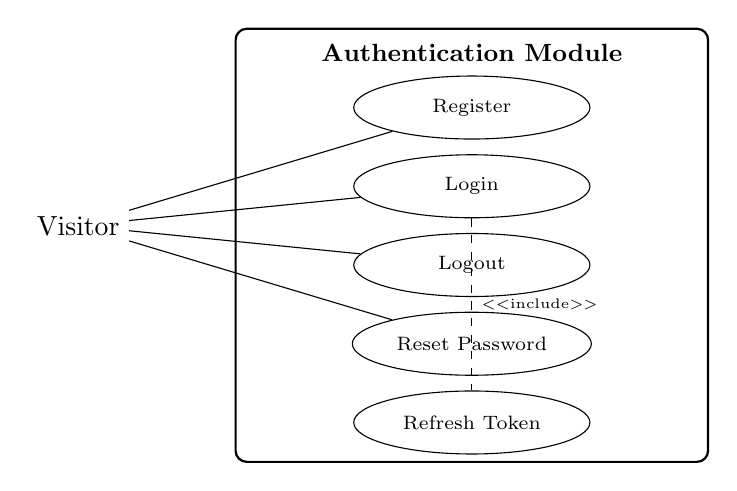
\begin{tikzpicture}[
  usecase/.style={draw, ellipse, minimum width=3cm, minimum height=0.8cm, align=center, font=\scriptsize}
]
  % System boundary
  \draw[thick, rounded corners] (0, -5) rectangle (6, 0.5);
  \node[font=\small\bfseries] at (3, 0.2) {Authentication Module};
  
  % Actor
  \node (visitor) at (-2, -2) {Visitor};
  
  % Use cases
  \node[usecase] (uc1) at (3, -0.5) {Register};
  \node[usecase] (uc2) at (3, -1.5) {Login};
  \node[usecase] (uc3) at (3, -2.5) {Logout};
  \node[usecase] (uc4) at (3, -3.5) {Reset Password};
  \node[usecase] (uc5) at (3, -4.5) {Refresh Token};
  
  % Arrows
  \draw (visitor) -- (uc1);
  \draw (visitor) -- (uc2);
  \draw (visitor) -- (uc3);
  \draw (visitor) -- (uc4);
  \draw[dashed] (uc2) -- node[right, font=\tiny] {<<include>>} (uc5);
  
\end{tikzpicture}
\caption{Use case diagram — Authentication}
\label{fig:uc-auth}
\end{figure}

\subsection{Sequence Diagram — Registration}

\begin{figure}[H]
\centering
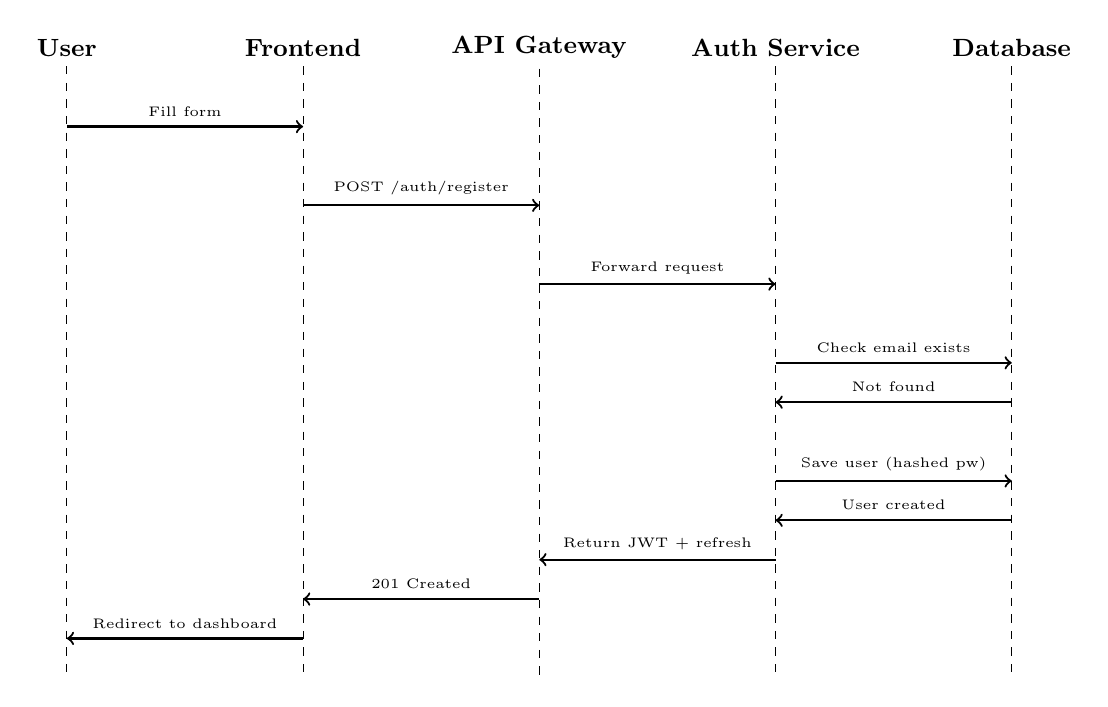
\begin{tikzpicture}[font=\small]
  % Lifelines
  \node (user) at (0, 0) {\textbf{User}};
  \node (front) at (3, 0) {\textbf{Frontend}};
  \node (gate) at (6, 0) {\textbf{API Gateway}};
  \node (auth) at (9, 0) {\textbf{Auth Service}};
  \node (db) at (12, 0) {\textbf{Database}};
  
  \draw[dashed] (user) -- (0, -8);
  \draw[dashed] (front) -- (3, -8);
  \draw[dashed] (gate) -- (6, -8);
  \draw[dashed] (auth) -- (9, -8);
  \draw[dashed] (db) -- (12, -8);
  
  % Messages
  \draw[->, thick] (0, -1) -- node[above, font=\tiny] {Fill form} (3, -1);
  \draw[->, thick] (3, -2) -- node[above, font=\tiny] {POST /auth/register} (6, -2);
  \draw[->, thick] (6, -3) -- node[above, font=\tiny] {Forward request} (9, -3);
  \draw[->, thick] (9, -4) -- node[above, font=\tiny] {Check email exists} (12, -4);
  \draw[<-, thick] (9, -4.5) -- node[above, font=\tiny] {Not found} (12, -4.5);
  \draw[->, thick] (9, -5.5) -- node[above, font=\tiny] {Save user (hashed pw)} (12, -5.5);
  \draw[<-, thick] (9, -6) -- node[above, font=\tiny] {User created} (12, -6);
  \draw[<-, thick] (6, -6.5) -- node[above, font=\tiny] {Return JWT + refresh} (9, -6.5);
  \draw[<-, thick] (3, -7) -- node[above, font=\tiny] {201 Created} (6, -7);
  \draw[<-, thick] (0, -7.5) -- node[above, font=\tiny] {Redirect to dashboard} (3, -7.5);
\end{tikzpicture}
\caption{Sequence diagram — User registration}
\label{fig:seq-register}
\end{figure}

\subsection{Sequence Diagram — Login}

\begin{figure}[H]
\centering
\begin{tikzpicture}[font=\small]
  % Lifelines
  \node (user) at (0, 0) {\textbf{User}};
  \node (front) at (3, 0) {\textbf{Frontend}};
  \node (gate) at (6, 0) {\textbf{API Gateway}};
  \node (auth) at (9, 0) {\textbf{Auth Service}};
  \node (db) at (12, 0) {\textbf{Database}};
  
  \draw[dashed] (user) -- (0, -8);
  \draw[dashed] (front) -- (3, -8);
  \draw[dashed] (gate) -- (6, -8);
  \draw[dashed] (auth) -- (9, -8);
  \draw[dashed] (db) -- (12, -8);
  
  % Messages
  \draw[->, thick] (0, -1) -- node[above, font=\tiny] {Enter credentials} (3, -1);
  \draw[->, thick] (3, -2) -- node[above, font=\tiny] {POST /auth/login} (6, -2);
  \draw[->, thick] (6, -3) -- node[above, font=\tiny] {Forward request} (9, -3);
  \draw[->, thick] (9, -4) -- node[above, font=\tiny] {Find user by email} (12, -4);
  \draw[<-, thick] (9, -4.5) -- node[above, font=\tiny] {User found} (12, -4.5);
  \draw[->, thick] (9, -5) -- node[right, font=\tiny] {Compare passwords};
  \draw[->, thick] (9, -5.5) -- node[right, font=\tiny] {Generate JWT + refresh};
  \draw[<-, thick] (6, -6) -- node[above, font=\tiny] {Return tokens} (9, -6);
  \draw[<-, thick] (3, -6.5) -- node[above, font=\tiny] {200 OK + tokens} (6, -6.5);
  \draw[<-, thick] (0, -7) -- node[above, font=\tiny] {Store token, redirect} (3, -7);
\end{tikzpicture}
\caption{Sequence diagram — User login}
\label{fig:seq-login}
\end{figure}

\subsection{Class Diagram — Auth Module}

\begin{figure}[H]
\centering
\begin{tikzpicture}[font=\small,
  class/.style={draw, rectangle, minimum width=4cm, align=left}
]
  % User class
  \node[class, fill=yellow!15] (userclass) at (0, 0) {
    \textbf{User}\\
    \hline
    - id: UUID\\
    - email: String\\
    - password: String\\
    - firstName: String\\
    - lastName: String\\
    - role: Role\\
    - createdAt: DateTime\\
    - updatedAt: DateTime\\
    \hline
    + register()\\
    + login()\\
    + resetPassword()
  };
  
  % Role enum
  \node[class, fill=green!15] (roleenum) at (6, 0) {
    \textbf{<<enum>> Role}\\
    \hline
    USER\\
    ADMIN
  };
  
  % RefreshToken class
  \node[class, fill=blue!15] (tokenclass) at (0, -5.5) {
    \textbf{RefreshToken}\\
    \hline
    - id: UUID\\
    - token: String\\
    - userId: UUID\\
    - expiresAt: DateTime\\
    - isRevoked: Boolean\\
    \hline
    + revoke()
  };
  
  % Relations
  \draw[->, thick] (userclass) -- node[above, font=\tiny] {has} (roleenum);
  \draw[->, thick] (userclass) -- node[left, font=\tiny] {has many} (tokenclass);
\end{tikzpicture}
\caption{Class diagram — Authentication module}
\label{fig:class-auth}
\end{figure}

\subsection{Implementation Screenshots}

% INSERT ACTUAL SCREENSHOTS HERE
\begin{figure}[H]
\centering
\fbox{\parbox{0.9\textwidth}{\centering\vspace{3cm}\textit{Insert registration page screenshot}\vspace{3cm}}}
\caption{Registration page}
\label{fig:register-page}
\end{figure}

\begin{figure}[H]
\centering
\fbox{\parbox{0.9\textwidth}{\centering\vspace{3cm}\textit{Insert login page screenshot}\vspace{3cm}}}
\caption{Login page}
\label{fig:login-page}
\end{figure}

\subsection{Sprint 2 Review}

At the end of Sprint 2, the following deliverables were achieved:
\begin{itemize}
  \item Complete auth service with registration, login, logout, password reset.
  \item JWT + refresh token implementation with role-based guards.
  \item Login and registration pages with form validation.
  \item OpenNebula installed and configured on the server.
  \item KVM hypervisor operational with VM templates.
\end{itemize}

% ============================================================
\section{Conclusion}

In this chapter, we completed the first two sprints. Sprint 1 established the project foundation with a modern landing page and Docker-based development environment. Sprint 2 delivered a complete authentication system with secure JWT-based access control. On the infrastructure side, OpenNebula was installed and configured for VM provisioning.

In the next chapter, we will cover Sprint 3 (User Management \& Dashboard) and Sprint 4 (VM Management \& Worker Service).

% ============================================================
\chapter{Sprint 1 \& Sprint 2: Foundation and Authentication}

\section{Introduction}

This chapter covers the first two sprints of the project. Sprint 1 focuses on establishing the project foundation and building the landing page, while Sprint 2 implements the authentication service with JWT-based security.

% ============================================================
% SPRINT 1
% ============================================================
\section{Sprint 1: Landing Page \& Project Foundation}

\sprintcard{1}{Landing Page \& Project Foundation}{Deliver a responsive landing page and set up the project skeleton with Docker containers.}

\subsection{Sprint Backlog}

\begin{longtable}{|c|p{5cm}|c|c|c|}
\hline
\rowcolor{blue!15}
\textbf{Task ID} & \textbf{Task} & \textbf{Assignee} & \textbf{Est.} & \textbf{Status} \\
\hline
\endhead
T-1.1 & Scaffold Next.js project & DSI & 2h & Done \\
\hline
T-1.2 & Scaffold NestJS microservices & DSI & 4h & Done \\
\hline
T-1.3 & Setup Docker Compose & DSI & 3h & Done \\
\hline
T-1.4 & Setup PostgreSQL + ORM & DSI & 3h & Done \\
\hline
T-1.5 & Landing page — Hero section & DSI & 4h & Done \\
\hline
T-1.6 & Landing page — Pricing section & DSI & 4h & Done \\
\hline
T-1.7 & Landing page — Features + Footer & DSI & 3h & Done \\
\hline
T-1.8 & Responsive design + Polish & DSI & 4h & Done \\
\hline
T-1.9 & Ubuntu Server hardening & RSI & 4h & Done \\
\hline
T-1.10 & Network configuration & RSI & 3h & Done \\
\hline
T-1.11 & Docker install on server & RSI & 2h & Done \\
\hline
T-1.12 & OpenNebula research & RSI & 6h & Done \\
\hline
\caption{Sprint 1 backlog}
\label{tab:sprint1-backlog}
\end{longtable}

\subsection{Mockups and Design}

% INSERT FIGMA SCREENSHOTS HERE
\begin{figure}[H]
\centering
% \includegraphics[width=\textwidth]{images/landing-mockup.png}
\fbox{\parbox{0.9\textwidth}{\centering\vspace{3cm}\textit{Insert Figma landing page mockup here}\vspace{3cm}}}
\caption{Landing page mockup (Figma)}
\label{fig:landing-mockup}
\end{figure}

\subsection{Implementation}

\subsubsection{Project Structure}

The project follows a monorepo structure with separate directories for each microservice:

\begin{lstlisting}[language=bash, caption={Project directory structure}]
cloudvm/
├── frontend/          # Next.js application
├── services/
│   ├── gateway/       # API Gateway (NestJS)
│   ├── auth/          # Auth Service (NestJS)
│   ├── user/          # User Service (NestJS)
│   ├── vm/            # VM Service (NestJS)
│   └── payment/       # Payment Service (NestJS)
├── worker/            # Python Worker
├── docker-compose.yml
└── .env
\end{lstlisting}

\subsubsection{Landing Page Screenshots}

% INSERT ACTUAL SCREENSHOTS HERE
\begin{figure}[H]
\centering
\fbox{\parbox{0.9\textwidth}{\centering\vspace{3cm}\textit{Insert landing page hero section screenshot}\vspace{3cm}}}
\caption{Landing page — Hero section}
\label{fig:landing-hero}
\end{figure}

\begin{figure}[H]
\centering
\fbox{\parbox{0.9\textwidth}{\centering\vspace{3cm}\textit{Insert landing page pricing section screenshot}\vspace{3cm}}}
\caption{Landing page — Pricing section}
\label{fig:landing-pricing}
\end{figure}

\subsection{Sprint 1 Review}

At the end of Sprint 1, the following deliverables were achieved:
\begin{itemize}
  \item Responsive landing page with hero, features, pricing, and footer sections.
  \item Docker Compose configuration with containers for all microservices.
  \item PostgreSQL database initialized with ORM configuration.
  \item Ubuntu Server hardened with SSH key authentication.
  \item Docker installed and configured on the server.
\end{itemize}


% ============================================================
% SPRINT 2
% ============================================================
\section{Sprint 2: Authentication Service}

\sprintcard{2}{Authentication Service}{Implement secure user registration, login, JWT authentication, and role-based access control.}

\subsection{Sprint Backlog}

\begin{longtable}{|c|p{5cm}|c|c|c|}
\hline
\rowcolor{blue!15}
\textbf{Task ID} & \textbf{Task} & \textbf{Assignee} & \textbf{Est.} & \textbf{Status} \\
\hline
\endhead
T-2.1 & Registration endpoint & DSI & 4h & Done \\
\hline
T-2.2 & Login endpoint & DSI & 4h & Done \\
\hline
T-2.3 & JWT + Refresh tokens & DSI & 4h & Done \\
\hline
T-2.4 & Logout + token blacklist & DSI & 2h & Done \\
\hline
T-2.5 & Password reset flow & DSI & 3h & Done \\
\hline
T-2.6 & Auth guards (JWT, Role) & DSI & 3h & Done \\
\hline
T-2.7 & Register page (frontend) & DSI & 4h & Done \\
\hline
T-2.8 & Login page (frontend) & DSI & 3h & Done \\
\hline
T-2.9 & Auth state management & DSI & 3h & Done \\
\hline
T-2.10 & OpenNebula installation & RSI & 6h & Done \\
\hline
T-2.11 & OpenNebula configuration & RSI & 6h & Done \\
\hline
T-2.12 & KVM setup + VM templates & RSI & 6h & Done \\
\hline
\caption{Sprint 2 backlog}
\label{tab:sprint2-backlog}
\end{longtable}

\subsection{Use Case Diagram — Authentication}

\begin{figure}[H]
\centering
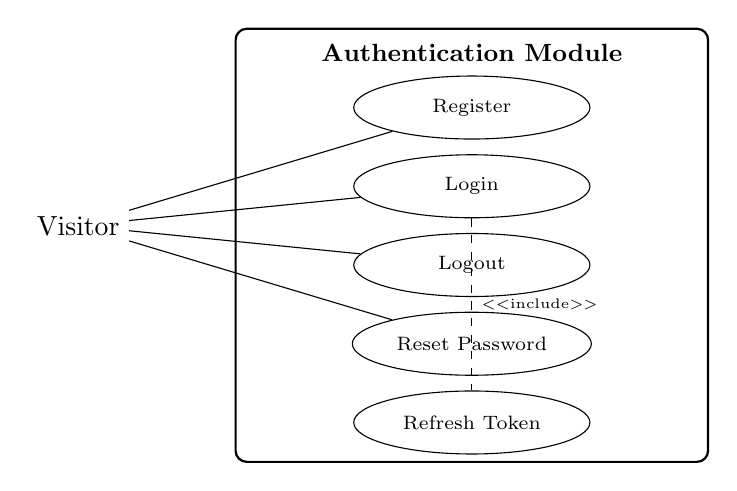
\begin{tikzpicture}[
  usecase/.style={draw, ellipse, minimum width=3cm, minimum height=0.8cm, align=center, font=\scriptsize}
]
  % System boundary
  \draw[thick, rounded corners] (0, -5) rectangle (6, 0.5);
  \node[font=\small\bfseries] at (3, 0.2) {Authentication Module};
  
  % Actor
  \node (visitor) at (-2, -2) {Visitor};
  
  % Use cases
  \node[usecase] (uc1) at (3, -0.5) {Register};
  \node[usecase] (uc2) at (3, -1.5) {Login};
  \node[usecase] (uc3) at (3, -2.5) {Logout};
  \node[usecase] (uc4) at (3, -3.5) {Reset Password};
  \node[usecase] (uc5) at (3, -4.5) {Refresh Token};
  
  % Arrows
  \draw (visitor) -- (uc1);
  \draw (visitor) -- (uc2);
  \draw (visitor) -- (uc3);
  \draw (visitor) -- (uc4);
  \draw[dashed] (uc2) -- node[right, font=\tiny] {<<include>>} (uc5);
  
\end{tikzpicture}
\caption{Use case diagram — Authentication}
\label{fig:uc-auth}
\end{figure}

\subsection{Sequence Diagram — Registration}

\begin{figure}[H]
\centering
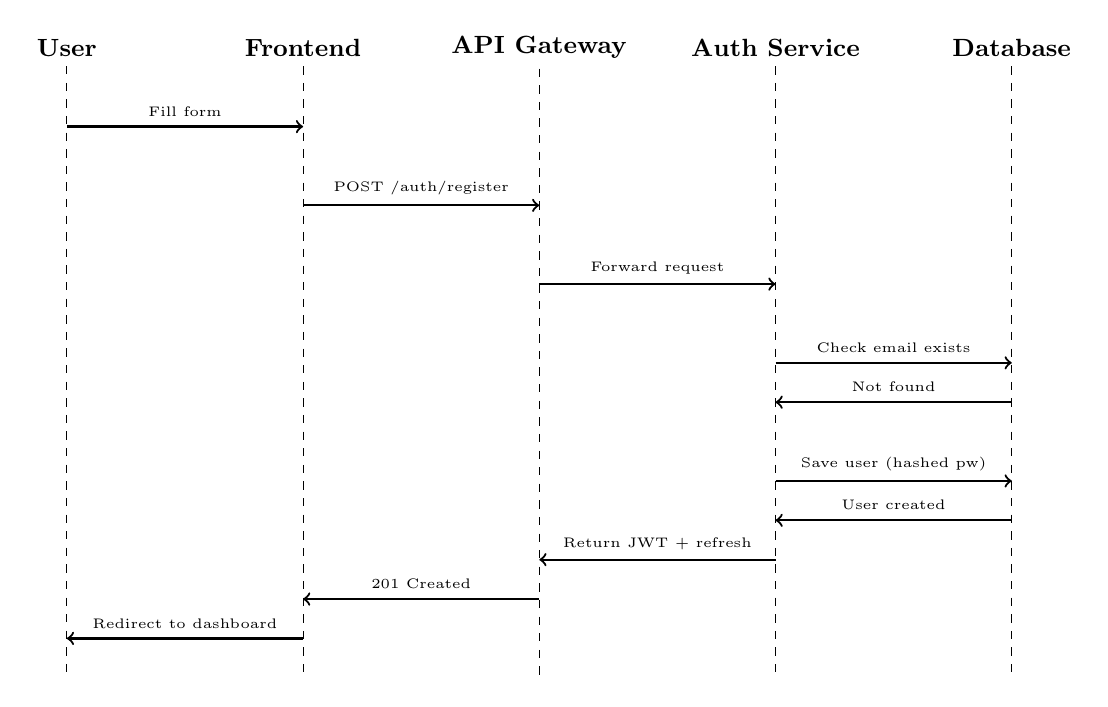
\begin{tikzpicture}[font=\small]
  % Lifelines
  \node (user) at (0, 0) {\textbf{User}};
  \node (front) at (3, 0) {\textbf{Frontend}};
  \node (gate) at (6, 0) {\textbf{API Gateway}};
  \node (auth) at (9, 0) {\textbf{Auth Service}};
  \node (db) at (12, 0) {\textbf{Database}};
  
  \draw[dashed] (user) -- (0, -8);
  \draw[dashed] (front) -- (3, -8);
  \draw[dashed] (gate) -- (6, -8);
  \draw[dashed] (auth) -- (9, -8);
  \draw[dashed] (db) -- (12, -8);
  
  % Messages
  \draw[->, thick] (0, -1) -- node[above, font=\tiny] {Fill form} (3, -1);
  \draw[->, thick] (3, -2) -- node[above, font=\tiny] {POST /auth/register} (6, -2);
  \draw[->, thick] (6, -3) -- node[above, font=\tiny] {Forward request} (9, -3);
  \draw[->, thick] (9, -4) -- node[above, font=\tiny] {Check email exists} (12, -4);
  \draw[<-, thick] (9, -4.5) -- node[above, font=\tiny] {Not found} (12, -4.5);
  \draw[->, thick] (9, -5.5) -- node[above, font=\tiny] {Save user (hashed pw)} (12, -5.5);
  \draw[<-, thick] (9, -6) -- node[above, font=\tiny] {User created} (12, -6);
  \draw[<-, thick] (6, -6.5) -- node[above, font=\tiny] {Return JWT + refresh} (9, -6.5);
  \draw[<-, thick] (3, -7) -- node[above, font=\tiny] {201 Created} (6, -7);
  \draw[<-, thick] (0, -7.5) -- node[above, font=\tiny] {Redirect to dashboard} (3, -7.5);
\end{tikzpicture}
\caption{Sequence diagram — User registration}
\label{fig:seq-register}
\end{figure}

\subsection{Sequence Diagram — Login}

\begin{figure}[H]
\centering
\begin{tikzpicture}[font=\small]
  % Lifelines
  \node (user) at (0, 0) {\textbf{User}};
  \node (front) at (3, 0) {\textbf{Frontend}};
  \node (gate) at (6, 0) {\textbf{API Gateway}};
  \node (auth) at (9, 0) {\textbf{Auth Service}};
  \node (db) at (12, 0) {\textbf{Database}};
  
  \draw[dashed] (user) -- (0, -8);
  \draw[dashed] (front) -- (3, -8);
  \draw[dashed] (gate) -- (6, -8);
  \draw[dashed] (auth) -- (9, -8);
  \draw[dashed] (db) -- (12, -8);
  
  % Messages
  \draw[->, thick] (0, -1) -- node[above, font=\tiny] {Enter credentials} (3, -1);
  \draw[->, thick] (3, -2) -- node[above, font=\tiny] {POST /auth/login} (6, -2);
  \draw[->, thick] (6, -3) -- node[above, font=\tiny] {Forward request} (9, -3);
  \draw[->, thick] (9, -4) -- node[above, font=\tiny] {Find user by email} (12, -4);
  \draw[<-, thick] (9, -4.5) -- node[above, font=\tiny] {User found} (12, -4.5);
  \draw[->, thick] (9, -5) -- node[right, font=\tiny] {Compare passwords};
  \draw[->, thick] (9, -5.5) -- node[right, font=\tiny] {Generate JWT + refresh};
  \draw[<-, thick] (6, -6) -- node[above, font=\tiny] {Return tokens} (9, -6);
  \draw[<-, thick] (3, -6.5) -- node[above, font=\tiny] {200 OK + tokens} (6, -6.5);
  \draw[<-, thick] (0, -7) -- node[above, font=\tiny] {Store token, redirect} (3, -7);
\end{tikzpicture}
\caption{Sequence diagram — User login}
\label{fig:seq-login}
\end{figure}

\subsection{Class Diagram — Auth Module}

\begin{figure}[H]
\centering
\begin{tikzpicture}[font=\small,
  class/.style={draw, rectangle, minimum width=4cm, align=left}
]
  % User class
  \node[class, fill=yellow!15] (userclass) at (0, 0) {
    \textbf{User}\\
    \hline
    - id: UUID\\
    - email: String\\
    - password: String\\
    - firstName: String\\
    - lastName: String\\
    - role: Role\\
    - createdAt: DateTime\\
    - updatedAt: DateTime\\
    \hline
    + register()\\
    + login()\\
    + resetPassword()
  };
  
  % Role enum
  \node[class, fill=green!15] (roleenum) at (6, 0) {
    \textbf{<<enum>> Role}\\
    \hline
    USER\\
    ADMIN
  };
  
  % RefreshToken class
  \node[class, fill=blue!15] (tokenclass) at (0, -5.5) {
    \textbf{RefreshToken}\\
    \hline
    - id: UUID\\
    - token: String\\
    - userId: UUID\\
    - expiresAt: DateTime\\
    - isRevoked: Boolean\\
    \hline
    + revoke()
  };
  
  % Relations
  \draw[->, thick] (userclass) -- node[above, font=\tiny] {has} (roleenum);
  \draw[->, thick] (userclass) -- node[left, font=\tiny] {has many} (tokenclass);
\end{tikzpicture}
\caption{Class diagram — Authentication module}
\label{fig:class-auth}
\end{figure}

\subsection{Implementation Screenshots}

% INSERT ACTUAL SCREENSHOTS HERE
\begin{figure}[H]
\centering
\fbox{\parbox{0.9\textwidth}{\centering\vspace{3cm}\textit{Insert registration page screenshot}\vspace{3cm}}}
\caption{Registration page}
\label{fig:register-page}
\end{figure}

\begin{figure}[H]
\centering
\fbox{\parbox{0.9\textwidth}{\centering\vspace{3cm}\textit{Insert login page screenshot}\vspace{3cm}}}
\caption{Login page}
\label{fig:login-page}
\end{figure}

\subsection{Sprint 2 Review}

At the end of Sprint 2, the following deliverables were achieved:
\begin{itemize}
  \item Complete auth service with registration, login, logout, password reset.
  \item JWT + refresh token implementation with role-based guards.
  \item Login and registration pages with form validation.
  \item OpenNebula installed and configured on the server.
  \item KVM hypervisor operational with VM templates.
\end{itemize}

% ============================================================
\section{Conclusion}

In this chapter, we completed the first two sprints. Sprint 1 established the project foundation with a modern landing page and Docker-based development environment. Sprint 2 delivered a complete authentication system with secure JWT-based access control. On the infrastructure side, OpenNebula was installed and configured for VM provisioning.

In the next chapter, we will cover Sprint 3 (User Management \& Dashboard) and Sprint 4 (VM Management \& Worker Service).


% ============================================================
% CHAPTER 3: Sprint 3 & 4 (Users + VMs)
% ============================================================
% % ============================================================
% CHAPTER 3: Sprint 3 & Sprint 4 — Users, Dashboard, VM Management
% ============================================================
% ADD THIS TO main.tex AFTER COMPLETING SPRINT 3 & 4
% Uncomment: % ============================================================
% CHAPTER 3: Sprint 3 & Sprint 4 — Users, Dashboard, VM Management
% ============================================================
% ADD THIS TO main.tex AFTER COMPLETING SPRINT 3 & 4
% Uncomment: % ============================================================
% CHAPTER 3: Sprint 3 & Sprint 4 — Users, Dashboard, VM Management
% ============================================================
% ADD THIS TO main.tex AFTER COMPLETING SPRINT 3 & 4
% Uncomment: \input{chapters/chapter3}
% ============================================================
\chapter{Sprint 3 \& Sprint 4: User Management and VM Operations}

\section{Introduction}

This chapter covers the core features of the platform. Sprint 3 implements user management, the dashboard layout, and NATS JetStream integration. Sprint 4 delivers the central feature — virtual machine lifecycle management through the VM service, Python worker, and OpenNebula integration.

% ============================================================
% SPRINT 3
% ============================================================
\section{Sprint 3: User Management \& Dashboard}

\sprintcard{3}{User Management \& Dashboard}{Implement user CRUD, admin management panel, dashboard layout, and message queue setup.}

\subsection{Sprint Backlog}

\begin{longtable}{|c|p{5cm}|c|c|c|}
\hline
\rowcolor{blue!15}
\textbf{Task ID} & \textbf{Task} & \textbf{Assignee} & \textbf{Est.} & \textbf{Status} \\
\hline
\endhead
T-3.1 & User service CRUD endpoints & DSI & 4h & Done \\
\hline
T-3.2 & Admin user management endpoints & DSI & 3h & Done \\
\hline
T-3.3 & Dashboard layout (sidebar, header) & DSI & 6h & Done \\
\hline
T-3.4 & Profile page (view/edit) & DSI & 4h & Done \\
\hline
T-3.11 & SSH key management (CRUD + UI) & DSI & 5h & Done \\
\hline
T-3.5 & Admin — user list page & DSI & 4h & Done \\
\hline
T-3.6 & NATS JetStream setup & DSI & 4h & Done \\
\hline
T-3.7 & Firewall rules (iptables) & RSI & 6h & Done \\
\hline
T-3.8 & Firewall testing & RSI & 4h & Done \\
\hline
T-3.9 & OpenNebula API access & RSI & 6h & Done \\
\hline
\caption{Sprint 3 backlog}
\label{tab:sprint3-backlog}
\end{longtable}

\subsection{Use Case Diagram — User Management}

\begin{figure}[H]
\centering
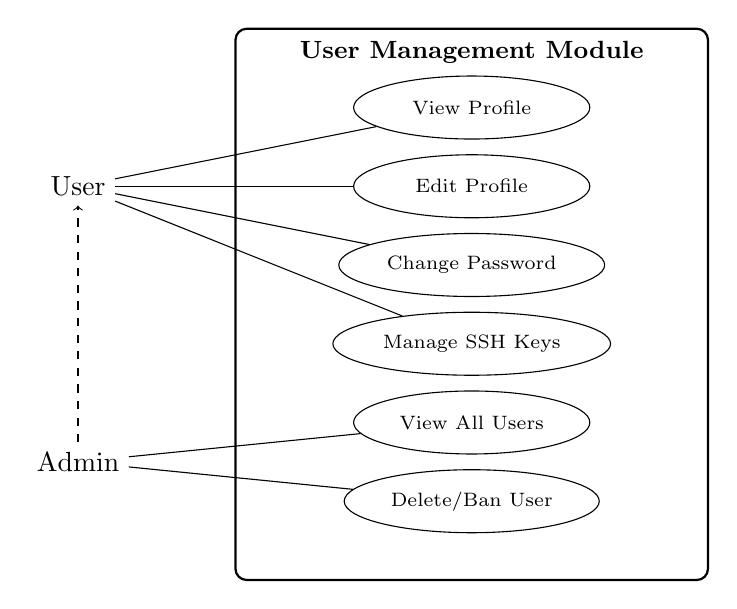
\begin{tikzpicture}[
  usecase/.style={draw, ellipse, minimum width=3cm, minimum height=0.8cm, align=center, font=\scriptsize}
]
  % System boundary
  \draw[thick, rounded corners] (0, -6.5) rectangle (6, 0.5);
  \node[font=\small\bfseries] at (3, 0.2) {User Management Module};
  
  % Actors
  \node (user) at (-2, -1.5) {User};
  \node (admin) at (-2, -5) {Admin};
  
  % Use cases
  \node[usecase] (uc1) at (3, -0.5) {View Profile};
  \node[usecase] (uc2) at (3, -1.5) {Edit Profile};
  \node[usecase] (uc3) at (3, -2.5) {Change Password};
  \node[usecase] (uc6) at (3, -3.5) {Manage SSH Keys};
  \node[usecase] (uc4) at (3, -4.5) {View All Users};
  \node[usecase] (uc5) at (3, -5.5) {Delete/Ban User};
  
  % Arrows
  \draw (user) -- (uc1);
  \draw (user) -- (uc2);
  \draw (user) -- (uc3);
  \draw (user) -- (uc6);
  \draw (admin) -- (uc4);
  \draw (admin) -- (uc5);
  
  % Generalization
  \draw[->, dashed] (admin) -- (user);
  
\end{tikzpicture}
\caption{Use case diagram — User management}
\label{fig:uc-user}
\end{figure}

\subsection{Sequence Diagram — Admin Deletes User}

\begin{figure}[H]
\centering
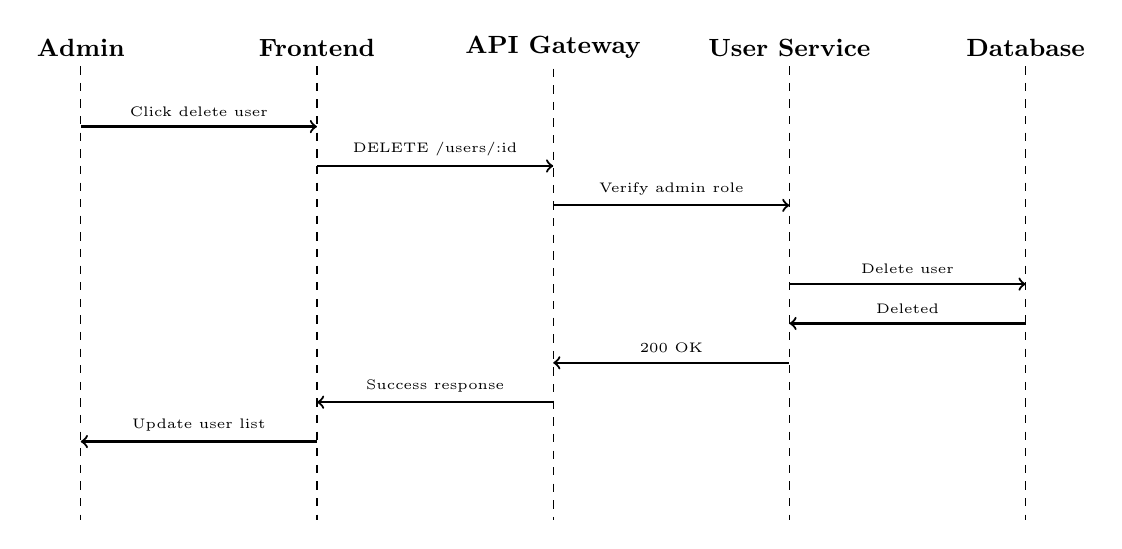
\begin{tikzpicture}[font=\small]
  \node (admin) at (0, 0) {\textbf{Admin}};
  \node (front) at (3, 0) {\textbf{Frontend}};
  \node (gate) at (6, 0) {\textbf{API Gateway}};
  \node (usvc) at (9, 0) {\textbf{User Service}};
  \node (db) at (12, 0) {\textbf{Database}};
  
  \draw[dashed] (admin) -- (0, -6);
  \draw[dashed] (front) -- (3, -6);
  \draw[dashed] (gate) -- (6, -6);
  \draw[dashed] (usvc) -- (9, -6);
  \draw[dashed] (db) -- (12, -6);
  
  \draw[->, thick] (0, -1) -- node[above, font=\tiny] {Click delete user} (3, -1);
  \draw[->, thick] (3, -1.5) -- node[above, font=\tiny] {DELETE /users/:id} (6, -1.5);
  \draw[->, thick] (6, -2) -- node[above, font=\tiny] {Verify admin role} (9, -2);
  \draw[->, thick] (9, -3) -- node[above, font=\tiny] {Delete user} (12, -3);
  \draw[<-, thick] (9, -3.5) -- node[above, font=\tiny] {Deleted} (12, -3.5);
  \draw[<-, thick] (6, -4) -- node[above, font=\tiny] {200 OK} (9, -4);
  \draw[<-, thick] (3, -4.5) -- node[above, font=\tiny] {Success response} (6, -4.5);
  \draw[<-, thick] (0, -5) -- node[above, font=\tiny] {Update user list} (3, -5);
\end{tikzpicture}
\caption{Sequence diagram — Admin deletes user}
\label{fig:seq-delete-user}
\end{figure}

\subsection{Implementation Screenshots}

\begin{figure}[H]
\centering
\fbox{\parbox{0.9\textwidth}{\centering\vspace{3cm}\textit{Insert dashboard layout screenshot}\vspace{3cm}}}
\caption{Dashboard layout with sidebar navigation}
\label{fig:dashboard-layout}
\end{figure}

\begin{figure}[H]
\centering
\fbox{\parbox{0.9\textwidth}{\centering\vspace{3cm}\textit{Insert admin user management screenshot}\vspace{3cm}}}
\caption{Admin — User management page}
\label{fig:admin-users}
\end{figure}

\begin{figure}[H]
\centering
\fbox{\parbox{0.9\textwidth}{\centering\vspace{3cm}\textit{Insert SSH key management page screenshot}\vspace{3cm}}}
\caption{SSH key management — User profile}
\label{fig:ssh-keys}
\end{figure}

\subsection{Sprint 3 Review}

At the end of Sprint 3:
\begin{itemize}
  \item User service with full CRUD operations.
  \item Admin panel for user management.
  \item Dashboard layout with sidebar, header, and responsive design.
  \item Profile page with edit functionality.
  \item SSH key management — users can add, view, and delete SSH public keys.
  \item NATS JetStream configured and tested.
  \item Firewall rules implemented and tested.
  \item OpenNebula XML-RPC API accessible and secured.
\end{itemize}


% ============================================================
% SPRINT 4
% ============================================================
\section{Sprint 4: VM Management \& Worker Service}

\sprintcard{4}{VM Management \& Worker Service}{Implement the core VM lifecycle operations — create, start, stop, reboot, delete — through the web platform with asynchronous processing via the Python worker.}

\subsection{Sprint Backlog}

\begin{longtable}{|c|p{5cm}|c|c|c|}
\hline
\rowcolor{blue!15}
\textbf{Task ID} & \textbf{Task} & \textbf{Assignee} & \textbf{Est.} & \textbf{Status} \\
\hline
\endhead
T-4.1 & VM service — Create VM endpoint & DSI & 5h & Done \\
\hline
T-4.2 & Python worker setup (Redis + NATS) & DSI & 5h & Done \\
\hline
T-4.3 & Worker — Create VM via OpenNebula & DSI & 5h & Done \\
\hline
T-4.4 & Worker — Start/Stop/Reboot ops & DSI & 4h & Done \\
\hline
T-4.5 & Worker — Delete VM operation & DSI & 2h & Done \\
\hline
T-4.6 & VM creation form (frontend) & DSI & 5h & Done \\
\hline
T-4.7 & VM list page (frontend) & DSI & 4h & Done \\
\hline
T-4.8 & OpenNebula API integration testing & RSI & 6h & Done \\
\hline
T-4.9 & VM networking (virtual networks) & RSI & 6h & Done \\
\hline
T-4.10 & Storage + disk images & RSI & 4h & Done \\
\hline
\caption{Sprint 4 backlog}
\label{tab:sprint4-backlog}
\end{longtable}

\subsection{Use Case Diagram — VM Management}

\begin{figure}[H]
\centering
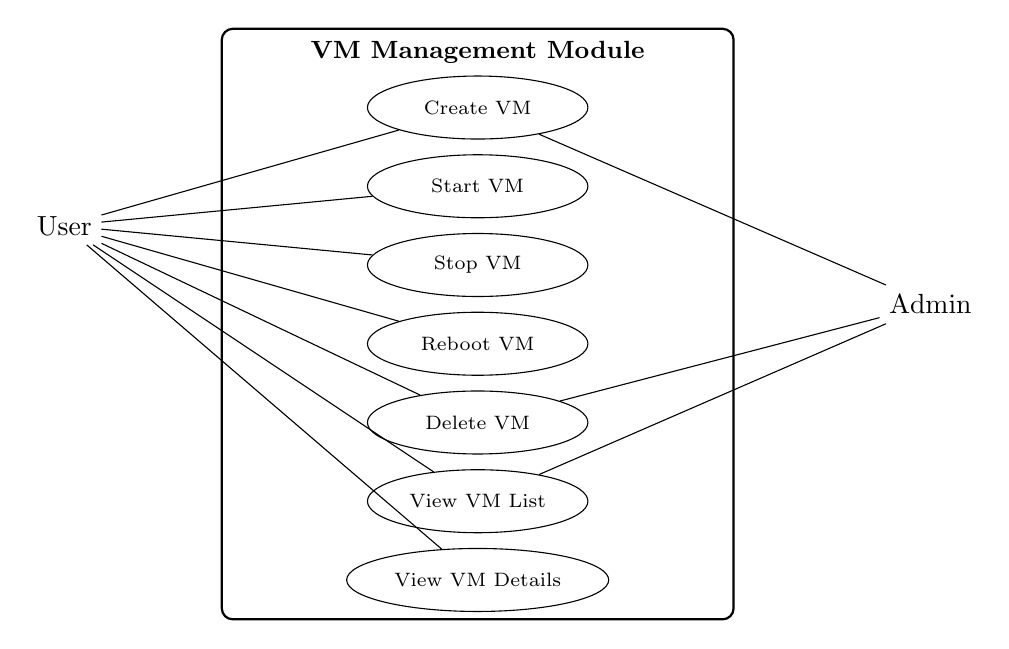
\begin{tikzpicture}[
  usecase/.style={draw, ellipse, minimum width=2.8cm, minimum height=0.8cm, align=center, font=\scriptsize}
]
  % System boundary
  \draw[thick, rounded corners] (0, -7) rectangle (6.5, 0.5);
  \node[font=\small\bfseries] at (3.25, 0.2) {VM Management Module};
  
  % Actors
  \node (user) at (-2, -2) {User};
  \node (admin) at (9, -3) {Admin};
  
  % Use cases
  \node[usecase] (uc1) at (3.25, -0.5) {Create VM};
  \node[usecase] (uc2) at (3.25, -1.5) {Start VM};
  \node[usecase] (uc3) at (3.25, -2.5) {Stop VM};
  \node[usecase] (uc4) at (3.25, -3.5) {Reboot VM};
  \node[usecase] (uc5) at (3.25, -4.5) {Delete VM};
  \node[usecase] (uc6) at (3.25, -5.5) {View VM List};
  \node[usecase] (uc7) at (3.25, -6.5) {View VM Details};
  
  % Arrows
  \draw (user) -- (uc1);
  \draw (user) -- (uc2);
  \draw (user) -- (uc3);
  \draw (user) -- (uc4);
  \draw (user) -- (uc5);
  \draw (user) -- (uc6);
  \draw (user) -- (uc7);
  
  \draw (admin) -- (uc1);
  \draw (admin) -- (uc5);
  \draw (admin) -- (uc6);
  
\end{tikzpicture}
\caption{Use case diagram — VM management}
\label{fig:uc-vm}
\end{figure}

\subsection{Sequence Diagram — VM Creation (End-to-End)}

\begin{figure}[H]
\centering
\begin{tikzpicture}[font=\scriptsize]
  % Lifelines
  \node (user) at (0, 0) {\textbf{User}};
  \node (front) at (2, 0) {\textbf{Frontend}};
  \node (gate) at (4, 0) {\textbf{Gateway}};
  \node (vmsvc) at (6, 0) {\textbf{VM Service}};
  \node (nats) at (8, 0) {\textbf{JetStream}};
  \node (worker) at (10, 0) {\textbf{Worker}};
  \node (one) at (12.5, 0) {\textbf{OpenNebula}};
  
  \draw[dashed] (user) -- (0, -11);
  \draw[dashed] (front) -- (2, -11);
  \draw[dashed] (gate) -- (4, -11);
  \draw[dashed] (vmsvc) -- (6, -11);
  \draw[dashed] (nats) -- (8, -11);
  \draw[dashed] (worker) -- (10, -11);
  \draw[dashed] (one) -- (12.5, -11);
  
  % Messages
  \draw[->, thick] (0, -0.8) -- node[above] {Fill VM form} (2, -0.8);
  \draw[->, thick] (2, -1.5) -- node[above] {POST /vms} (4, -1.5);
  \draw[->, thick] (4, -2.2) -- node[above] {Forward} (6, -2.2);
  \draw[->, thick] (6, -2.7) -- node[right] {Check quota};
  \draw[->, thick] (6, -3.5) -- node[above] {Save VM (pending)} (6, -3.5);
  \draw[->, thick] (6, -4.2) -- node[above] {Publish event} (8, -4.2);
  \draw[<-, thick] (4, -4.9) -- node[above] {202 Accepted} (6, -4.9);
  \draw[<-, thick] (2, -5.3) -- node[above] {VM creating...} (4, -5.3);
  \draw[->, thick] (8, -6) -- node[above] {Consume event} (10, -6);
  \draw[->, thick] (10, -6.7) -- node[above] {Create VM} (12.5, -6.7);
  \draw[<-, thick] (10, -7.4) -- node[above] {VM ID + IP} (12.5, -7.4);
  \draw[->, thick] (10, -8.1) -- node[above] {Publish result} (8, -8.1);
  \draw[->, thick] (6, -8.8) -- node[above] {Update status} (6, -8.8);
  \draw[->, thick] (6, -9) -- node[right] {VM → running};
  \draw[<-, thick] (2, -9.7) -- node[above] {Status update} (6, -9.7);
  \draw[<-, thick] (0, -10.3) -- node[above] {VM ready!} (2, -10.3);
\end{tikzpicture}
\caption{Sequence diagram — VM creation (end-to-end)}
\label{fig:seq-vm-create}
\end{figure}

\subsection{Activity Diagram — VM Lifecycle}

\begin{figure}[H]
\centering
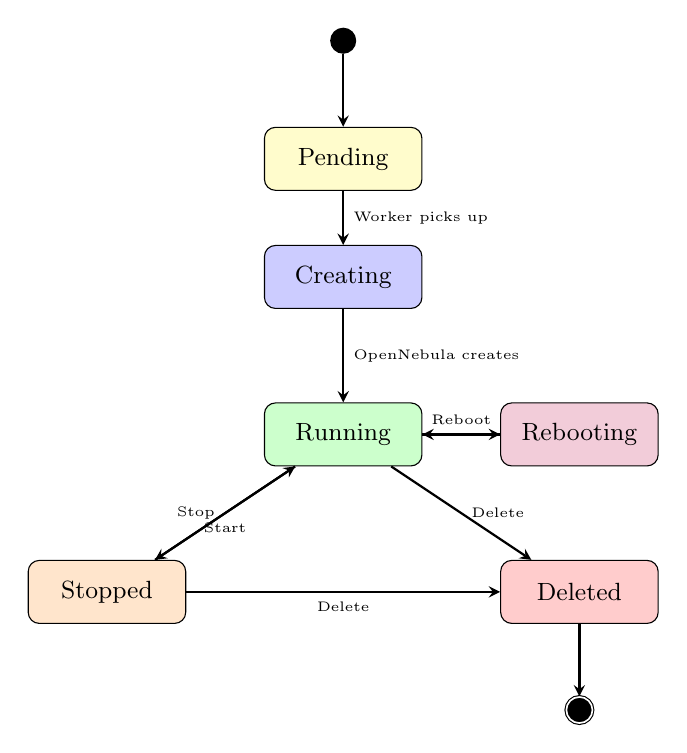
\begin{tikzpicture}[
  state/.style={draw, rounded corners, minimum width=2cm, minimum height=0.8cm, align=center, font=\small},
  decision/.style={draw, diamond, minimum width=1.5cm, minimum height=1cm, align=center, font=\tiny},
  arrow/.style={->, thick, >=stealth}
]
  % States
  \node[circle, fill=black, minimum size=0.3cm] (start) at (0, 0) {};
  \node[state, fill=yellow!20] (pending) at (0, -1.5) {Pending};
  \node[state, fill=blue!20] (creating) at (0, -3) {Creating};
  \node[state, fill=green!20] (running) at (0, -5) {Running};
  \node[state, fill=orange!20] (stopped) at (-3, -7) {Stopped};
  \node[state, fill=red!20] (deleted) at (3, -7) {Deleted};
  \node[state, fill=purple!20] (rebooting) at (3, -5) {Rebooting};
  \node[circle, draw, fill=black, minimum size=0.3cm, double] (end) at (3, -8.5) {};
  
  % Arrows
  \draw[arrow] (start) -- (pending);
  \draw[arrow] (pending) -- node[right, font=\tiny] {Worker picks up} (creating);
  \draw[arrow] (creating) -- node[right, font=\tiny] {OpenNebula creates} (running);
  \draw[arrow] (running) -- node[left, font=\tiny] {Stop} (stopped);
  \draw[arrow] (stopped) -- node[below, font=\tiny] {Start} (running);
  \draw[arrow] (running) -- node[above, font=\tiny] {Reboot} (rebooting);
  \draw[arrow] (rebooting) -- node[right, font=\tiny] {} (running);
  \draw[arrow] (running) -- node[right, font=\tiny] {Delete} (deleted);
  \draw[arrow] (stopped) -- node[below, font=\tiny] {Delete} (deleted);
  \draw[arrow] (deleted) -- (end);
\end{tikzpicture}
\caption{Activity diagram — VM lifecycle}
\label{fig:activity-vm}
\end{figure}

\subsection{Class Diagram — VM Module}

\begin{figure}[H]
\centering
\begin{tikzpicture}[font=\small,
  class/.style={draw, rectangle, minimum width=4cm, align=left}
]
  % VM class
  \node[class, fill=yellow!15] (vmclass) at (0, 0) {
    \textbf{VirtualMachine}\\
    \hline
    - id: UUID\\
    - name: String\\
    - userId: UUID\\
    - templateId: String\\
    - vcpu: Integer\\
    - ram: Integer (MB)\\
    - disk: Integer (GB)\\
    - status: VMStatus\\
    - ipAddress: String\\
    - oneId: Integer\\
    - createdAt: DateTime\\
    \hline
    + create()\\
    + start()\\
    + stop()\\
    + reboot()\\
    + delete()
  };
  
  % VMStatus enum
  \node[class, fill=green!15] (statusenum) at (6, 1) {
    \textbf{<<enum>> VMStatus}\\
    \hline
    PENDING\\
    CREATING\\
    RUNNING\\
    STOPPED\\
    REBOOTING\\
    DELETING\\
    DELETED\\
    ERROR
  };
  
  % VMTemplate
  \node[class, fill=blue!15] (template) at (6, -3.5) {
    \textbf{VMTemplate}\\
    \hline
    - id: String\\
    - name: String\\
    - os: String\\
    - minCpu: Integer\\
    - minRam: Integer\\
    - minDisk: Integer\\
    \hline
    + getTemplates()
  };
  
  % Relations
  \draw[->, thick] (vmclass) -- node[above, font=\tiny] {has} (statusenum);
  \draw[->, thick] (vmclass) -- node[below, font=\tiny] {uses} (template);
\end{tikzpicture}
\caption{Class diagram — VM module}
\label{fig:class-vm}
\end{figure}

\subsection{Architecture Diagram — Worker Communication}

\begin{figure}[H]
\centering
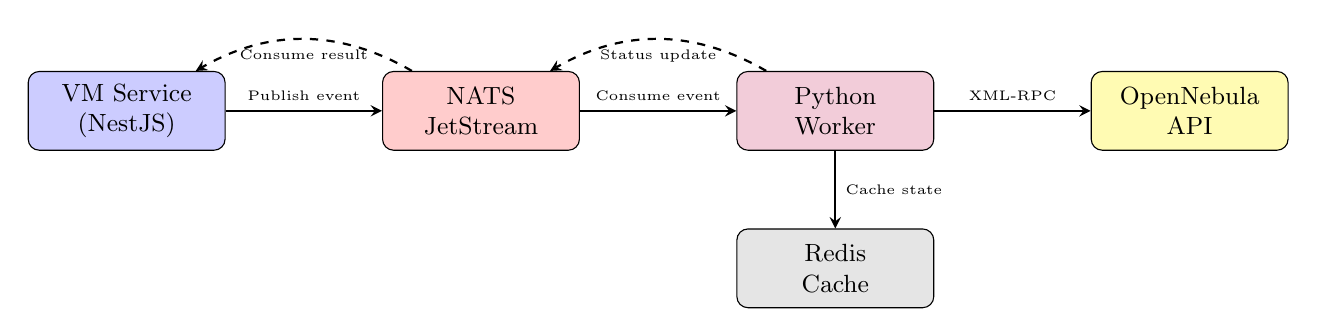
\begin{tikzpicture}[
  box/.style={draw, rounded corners, minimum width=2.5cm, minimum height=1cm, align=center, font=\small},
  arrow/.style={->, thick, >=stealth}
]
  \node[box, fill=blue!20] (vmsvc) at (0, 0) {VM Service\\(NestJS)};
  \node[box, fill=red!20] (nats) at (4.5, 0) {NATS\\JetStream};
  \node[box, fill=purple!20] (worker) at (9, 0) {Python\\Worker};
  \node[box, fill=gray!20] (redis) at (9, -2) {Redis\\Cache};
  \node[box, fill=yellow!30] (one) at (13.5, 0) {OpenNebula\\API};
  
  \draw[arrow] (vmsvc) -- node[above, font=\tiny] {Publish event} (nats);
  \draw[arrow] (nats) -- node[above, font=\tiny] {Consume event} (worker);
  \draw[arrow] (worker) -- node[above, font=\tiny] {XML-RPC} (one);
  \draw[arrow] (worker) -- node[right, font=\tiny] {Cache state} (redis);
  \draw[arrow, dashed] (worker) to[bend right=30] node[below, font=\tiny] {Status update} (nats);
  \draw[arrow, dashed] (nats) to[bend right=30] node[below, font=\tiny] {Consume result} (vmsvc);
\end{tikzpicture}
\caption{Architecture — Worker communication via JetStream}
\label{fig:worker-arch}
\end{figure}

\subsection{Implementation Screenshots}

\begin{figure}[H]
\centering
\fbox{\parbox{0.9\textwidth}{\centering\vspace{3cm}\textit{Insert VM creation form screenshot}\vspace{3cm}}}
\caption{VM creation form}
\label{fig:vm-create-form}
\end{figure}

\begin{figure}[H]
\centering
\fbox{\parbox{0.9\textwidth}{\centering\vspace{3cm}\textit{Insert VM list page screenshot}\vspace{3cm}}}
\caption{VM list page}
\label{fig:vm-list}
\end{figure}

\subsection{Sprint 4 Review}

At the end of Sprint 4:
\begin{itemize}
  \item VM service with full lifecycle operations (create, start, stop, reboot, delete).
  \item Python worker consuming events from NATS JetStream.
  \item Worker communicates with OpenNebula via XML-RPC API.
  \item VM creation form with template selection.
  \item VM list page with status indicators.
  \item OpenNebula virtual networks and storage configured.
  \item End-to-end VM creation working.
\end{itemize}

% ============================================================
\section{Conclusion}

In this chapter, we completed the user management features and the core VM operations. Sprint 3 delivered the admin panel, dashboard layout, and message queue infrastructure. Sprint 4 implemented the central feature of the platform — the ability to create and manage virtual machines through an asynchronous worker that communicates with OpenNebula.

In the next chapter, we will enhance the VM experience with a detailed dashboard, implement the quota system, and build the payment service.

% ============================================================
\chapter{Sprint 3 \& Sprint 4: User Management and VM Operations}

\section{Introduction}

This chapter covers the core features of the platform. Sprint 3 implements user management, the dashboard layout, and NATS JetStream integration. Sprint 4 delivers the central feature — virtual machine lifecycle management through the VM service, Python worker, and OpenNebula integration.

% ============================================================
% SPRINT 3
% ============================================================
\section{Sprint 3: User Management \& Dashboard}

\sprintcard{3}{User Management \& Dashboard}{Implement user CRUD, admin management panel, dashboard layout, and message queue setup.}

\subsection{Sprint Backlog}

\begin{longtable}{|c|p{5cm}|c|c|c|}
\hline
\rowcolor{blue!15}
\textbf{Task ID} & \textbf{Task} & \textbf{Assignee} & \textbf{Est.} & \textbf{Status} \\
\hline
\endhead
T-3.1 & User service CRUD endpoints & DSI & 4h & Done \\
\hline
T-3.2 & Admin user management endpoints & DSI & 3h & Done \\
\hline
T-3.3 & Dashboard layout (sidebar, header) & DSI & 6h & Done \\
\hline
T-3.4 & Profile page (view/edit) & DSI & 4h & Done \\
\hline
T-3.11 & SSH key management (CRUD + UI) & DSI & 5h & Done \\
\hline
T-3.5 & Admin — user list page & DSI & 4h & Done \\
\hline
T-3.6 & NATS JetStream setup & DSI & 4h & Done \\
\hline
T-3.7 & Firewall rules (iptables) & RSI & 6h & Done \\
\hline
T-3.8 & Firewall testing & RSI & 4h & Done \\
\hline
T-3.9 & OpenNebula API access & RSI & 6h & Done \\
\hline
\caption{Sprint 3 backlog}
\label{tab:sprint3-backlog}
\end{longtable}

\subsection{Use Case Diagram — User Management}

\begin{figure}[H]
\centering
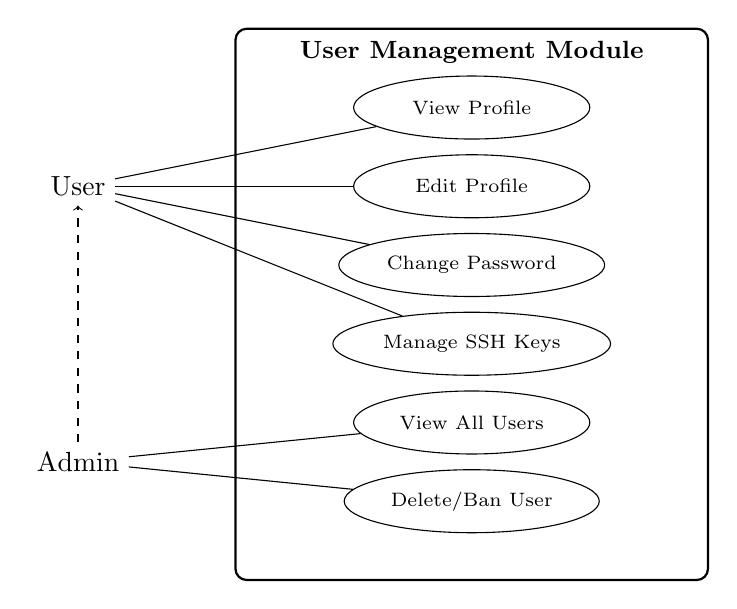
\begin{tikzpicture}[
  usecase/.style={draw, ellipse, minimum width=3cm, minimum height=0.8cm, align=center, font=\scriptsize}
]
  % System boundary
  \draw[thick, rounded corners] (0, -6.5) rectangle (6, 0.5);
  \node[font=\small\bfseries] at (3, 0.2) {User Management Module};
  
  % Actors
  \node (user) at (-2, -1.5) {User};
  \node (admin) at (-2, -5) {Admin};
  
  % Use cases
  \node[usecase] (uc1) at (3, -0.5) {View Profile};
  \node[usecase] (uc2) at (3, -1.5) {Edit Profile};
  \node[usecase] (uc3) at (3, -2.5) {Change Password};
  \node[usecase] (uc6) at (3, -3.5) {Manage SSH Keys};
  \node[usecase] (uc4) at (3, -4.5) {View All Users};
  \node[usecase] (uc5) at (3, -5.5) {Delete/Ban User};
  
  % Arrows
  \draw (user) -- (uc1);
  \draw (user) -- (uc2);
  \draw (user) -- (uc3);
  \draw (user) -- (uc6);
  \draw (admin) -- (uc4);
  \draw (admin) -- (uc5);
  
  % Generalization
  \draw[->, dashed] (admin) -- (user);
  
\end{tikzpicture}
\caption{Use case diagram — User management}
\label{fig:uc-user}
\end{figure}

\subsection{Sequence Diagram — Admin Deletes User}

\begin{figure}[H]
\centering
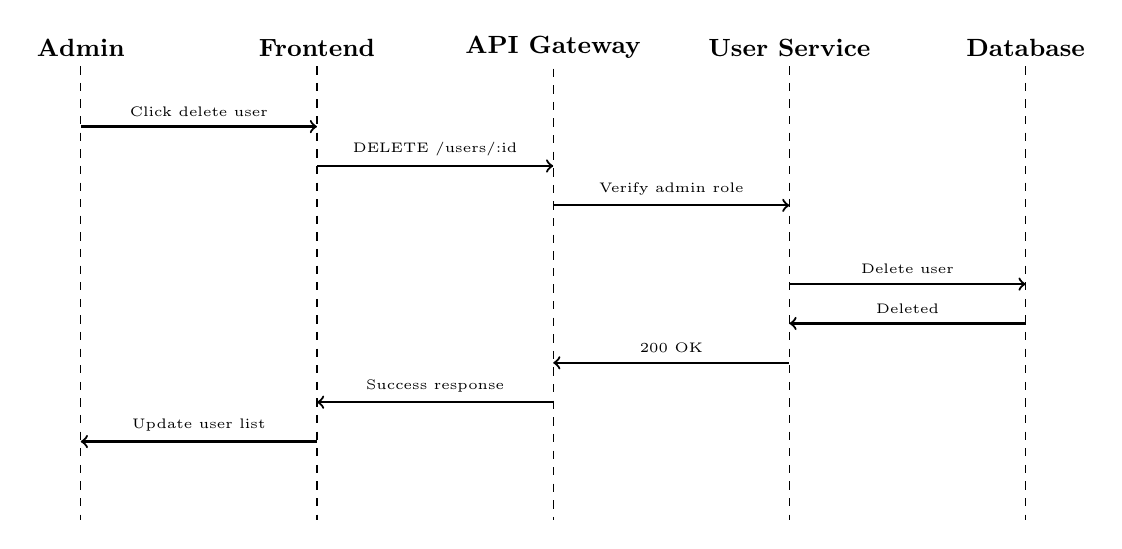
\begin{tikzpicture}[font=\small]
  \node (admin) at (0, 0) {\textbf{Admin}};
  \node (front) at (3, 0) {\textbf{Frontend}};
  \node (gate) at (6, 0) {\textbf{API Gateway}};
  \node (usvc) at (9, 0) {\textbf{User Service}};
  \node (db) at (12, 0) {\textbf{Database}};
  
  \draw[dashed] (admin) -- (0, -6);
  \draw[dashed] (front) -- (3, -6);
  \draw[dashed] (gate) -- (6, -6);
  \draw[dashed] (usvc) -- (9, -6);
  \draw[dashed] (db) -- (12, -6);
  
  \draw[->, thick] (0, -1) -- node[above, font=\tiny] {Click delete user} (3, -1);
  \draw[->, thick] (3, -1.5) -- node[above, font=\tiny] {DELETE /users/:id} (6, -1.5);
  \draw[->, thick] (6, -2) -- node[above, font=\tiny] {Verify admin role} (9, -2);
  \draw[->, thick] (9, -3) -- node[above, font=\tiny] {Delete user} (12, -3);
  \draw[<-, thick] (9, -3.5) -- node[above, font=\tiny] {Deleted} (12, -3.5);
  \draw[<-, thick] (6, -4) -- node[above, font=\tiny] {200 OK} (9, -4);
  \draw[<-, thick] (3, -4.5) -- node[above, font=\tiny] {Success response} (6, -4.5);
  \draw[<-, thick] (0, -5) -- node[above, font=\tiny] {Update user list} (3, -5);
\end{tikzpicture}
\caption{Sequence diagram — Admin deletes user}
\label{fig:seq-delete-user}
\end{figure}

\subsection{Implementation Screenshots}

\begin{figure}[H]
\centering
\fbox{\parbox{0.9\textwidth}{\centering\vspace{3cm}\textit{Insert dashboard layout screenshot}\vspace{3cm}}}
\caption{Dashboard layout with sidebar navigation}
\label{fig:dashboard-layout}
\end{figure}

\begin{figure}[H]
\centering
\fbox{\parbox{0.9\textwidth}{\centering\vspace{3cm}\textit{Insert admin user management screenshot}\vspace{3cm}}}
\caption{Admin — User management page}
\label{fig:admin-users}
\end{figure}

\begin{figure}[H]
\centering
\fbox{\parbox{0.9\textwidth}{\centering\vspace{3cm}\textit{Insert SSH key management page screenshot}\vspace{3cm}}}
\caption{SSH key management — User profile}
\label{fig:ssh-keys}
\end{figure}

\subsection{Sprint 3 Review}

At the end of Sprint 3:
\begin{itemize}
  \item User service with full CRUD operations.
  \item Admin panel for user management.
  \item Dashboard layout with sidebar, header, and responsive design.
  \item Profile page with edit functionality.
  \item SSH key management — users can add, view, and delete SSH public keys.
  \item NATS JetStream configured and tested.
  \item Firewall rules implemented and tested.
  \item OpenNebula XML-RPC API accessible and secured.
\end{itemize}


% ============================================================
% SPRINT 4
% ============================================================
\section{Sprint 4: VM Management \& Worker Service}

\sprintcard{4}{VM Management \& Worker Service}{Implement the core VM lifecycle operations — create, start, stop, reboot, delete — through the web platform with asynchronous processing via the Python worker.}

\subsection{Sprint Backlog}

\begin{longtable}{|c|p{5cm}|c|c|c|}
\hline
\rowcolor{blue!15}
\textbf{Task ID} & \textbf{Task} & \textbf{Assignee} & \textbf{Est.} & \textbf{Status} \\
\hline
\endhead
T-4.1 & VM service — Create VM endpoint & DSI & 5h & Done \\
\hline
T-4.2 & Python worker setup (Redis + NATS) & DSI & 5h & Done \\
\hline
T-4.3 & Worker — Create VM via OpenNebula & DSI & 5h & Done \\
\hline
T-4.4 & Worker — Start/Stop/Reboot ops & DSI & 4h & Done \\
\hline
T-4.5 & Worker — Delete VM operation & DSI & 2h & Done \\
\hline
T-4.6 & VM creation form (frontend) & DSI & 5h & Done \\
\hline
T-4.7 & VM list page (frontend) & DSI & 4h & Done \\
\hline
T-4.8 & OpenNebula API integration testing & RSI & 6h & Done \\
\hline
T-4.9 & VM networking (virtual networks) & RSI & 6h & Done \\
\hline
T-4.10 & Storage + disk images & RSI & 4h & Done \\
\hline
\caption{Sprint 4 backlog}
\label{tab:sprint4-backlog}
\end{longtable}

\subsection{Use Case Diagram — VM Management}

\begin{figure}[H]
\centering
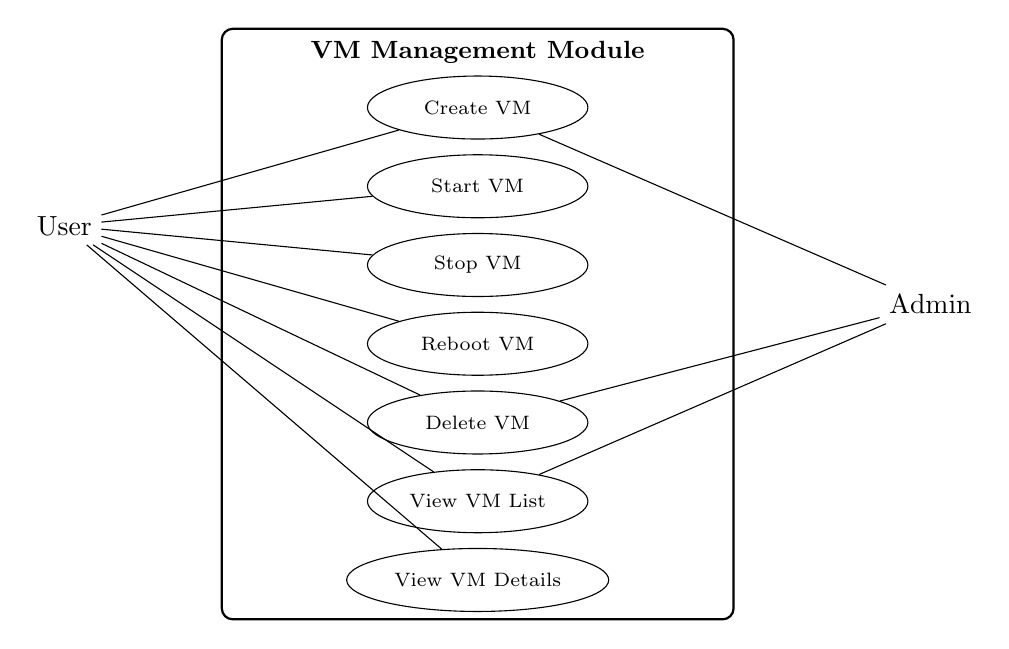
\begin{tikzpicture}[
  usecase/.style={draw, ellipse, minimum width=2.8cm, minimum height=0.8cm, align=center, font=\scriptsize}
]
  % System boundary
  \draw[thick, rounded corners] (0, -7) rectangle (6.5, 0.5);
  \node[font=\small\bfseries] at (3.25, 0.2) {VM Management Module};
  
  % Actors
  \node (user) at (-2, -2) {User};
  \node (admin) at (9, -3) {Admin};
  
  % Use cases
  \node[usecase] (uc1) at (3.25, -0.5) {Create VM};
  \node[usecase] (uc2) at (3.25, -1.5) {Start VM};
  \node[usecase] (uc3) at (3.25, -2.5) {Stop VM};
  \node[usecase] (uc4) at (3.25, -3.5) {Reboot VM};
  \node[usecase] (uc5) at (3.25, -4.5) {Delete VM};
  \node[usecase] (uc6) at (3.25, -5.5) {View VM List};
  \node[usecase] (uc7) at (3.25, -6.5) {View VM Details};
  
  % Arrows
  \draw (user) -- (uc1);
  \draw (user) -- (uc2);
  \draw (user) -- (uc3);
  \draw (user) -- (uc4);
  \draw (user) -- (uc5);
  \draw (user) -- (uc6);
  \draw (user) -- (uc7);
  
  \draw (admin) -- (uc1);
  \draw (admin) -- (uc5);
  \draw (admin) -- (uc6);
  
\end{tikzpicture}
\caption{Use case diagram — VM management}
\label{fig:uc-vm}
\end{figure}

\subsection{Sequence Diagram — VM Creation (End-to-End)}

\begin{figure}[H]
\centering
\begin{tikzpicture}[font=\scriptsize]
  % Lifelines
  \node (user) at (0, 0) {\textbf{User}};
  \node (front) at (2, 0) {\textbf{Frontend}};
  \node (gate) at (4, 0) {\textbf{Gateway}};
  \node (vmsvc) at (6, 0) {\textbf{VM Service}};
  \node (nats) at (8, 0) {\textbf{JetStream}};
  \node (worker) at (10, 0) {\textbf{Worker}};
  \node (one) at (12.5, 0) {\textbf{OpenNebula}};
  
  \draw[dashed] (user) -- (0, -11);
  \draw[dashed] (front) -- (2, -11);
  \draw[dashed] (gate) -- (4, -11);
  \draw[dashed] (vmsvc) -- (6, -11);
  \draw[dashed] (nats) -- (8, -11);
  \draw[dashed] (worker) -- (10, -11);
  \draw[dashed] (one) -- (12.5, -11);
  
  % Messages
  \draw[->, thick] (0, -0.8) -- node[above] {Fill VM form} (2, -0.8);
  \draw[->, thick] (2, -1.5) -- node[above] {POST /vms} (4, -1.5);
  \draw[->, thick] (4, -2.2) -- node[above] {Forward} (6, -2.2);
  \draw[->, thick] (6, -2.7) -- node[right] {Check quota};
  \draw[->, thick] (6, -3.5) -- node[above] {Save VM (pending)} (6, -3.5);
  \draw[->, thick] (6, -4.2) -- node[above] {Publish event} (8, -4.2);
  \draw[<-, thick] (4, -4.9) -- node[above] {202 Accepted} (6, -4.9);
  \draw[<-, thick] (2, -5.3) -- node[above] {VM creating...} (4, -5.3);
  \draw[->, thick] (8, -6) -- node[above] {Consume event} (10, -6);
  \draw[->, thick] (10, -6.7) -- node[above] {Create VM} (12.5, -6.7);
  \draw[<-, thick] (10, -7.4) -- node[above] {VM ID + IP} (12.5, -7.4);
  \draw[->, thick] (10, -8.1) -- node[above] {Publish result} (8, -8.1);
  \draw[->, thick] (6, -8.8) -- node[above] {Update status} (6, -8.8);
  \draw[->, thick] (6, -9) -- node[right] {VM → running};
  \draw[<-, thick] (2, -9.7) -- node[above] {Status update} (6, -9.7);
  \draw[<-, thick] (0, -10.3) -- node[above] {VM ready!} (2, -10.3);
\end{tikzpicture}
\caption{Sequence diagram — VM creation (end-to-end)}
\label{fig:seq-vm-create}
\end{figure}

\subsection{Activity Diagram — VM Lifecycle}

\begin{figure}[H]
\centering
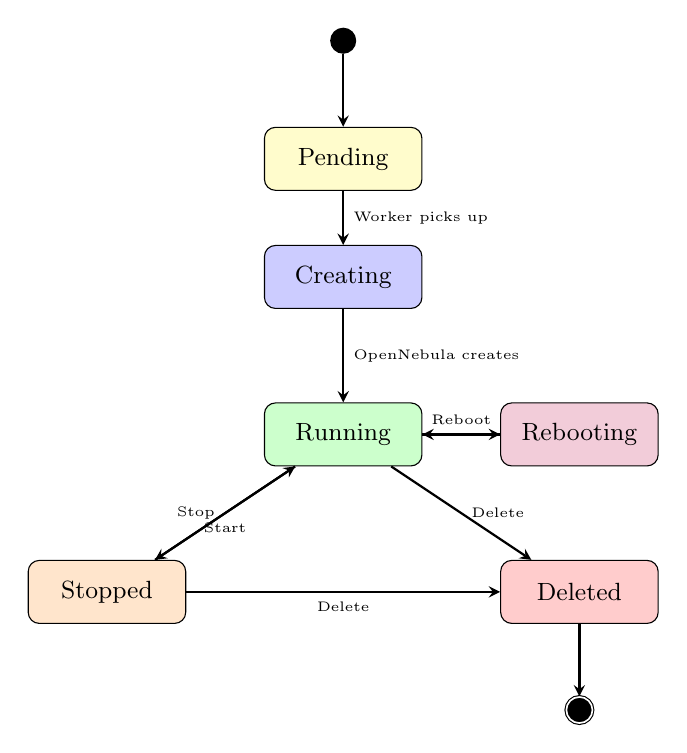
\begin{tikzpicture}[
  state/.style={draw, rounded corners, minimum width=2cm, minimum height=0.8cm, align=center, font=\small},
  decision/.style={draw, diamond, minimum width=1.5cm, minimum height=1cm, align=center, font=\tiny},
  arrow/.style={->, thick, >=stealth}
]
  % States
  \node[circle, fill=black, minimum size=0.3cm] (start) at (0, 0) {};
  \node[state, fill=yellow!20] (pending) at (0, -1.5) {Pending};
  \node[state, fill=blue!20] (creating) at (0, -3) {Creating};
  \node[state, fill=green!20] (running) at (0, -5) {Running};
  \node[state, fill=orange!20] (stopped) at (-3, -7) {Stopped};
  \node[state, fill=red!20] (deleted) at (3, -7) {Deleted};
  \node[state, fill=purple!20] (rebooting) at (3, -5) {Rebooting};
  \node[circle, draw, fill=black, minimum size=0.3cm, double] (end) at (3, -8.5) {};
  
  % Arrows
  \draw[arrow] (start) -- (pending);
  \draw[arrow] (pending) -- node[right, font=\tiny] {Worker picks up} (creating);
  \draw[arrow] (creating) -- node[right, font=\tiny] {OpenNebula creates} (running);
  \draw[arrow] (running) -- node[left, font=\tiny] {Stop} (stopped);
  \draw[arrow] (stopped) -- node[below, font=\tiny] {Start} (running);
  \draw[arrow] (running) -- node[above, font=\tiny] {Reboot} (rebooting);
  \draw[arrow] (rebooting) -- node[right, font=\tiny] {} (running);
  \draw[arrow] (running) -- node[right, font=\tiny] {Delete} (deleted);
  \draw[arrow] (stopped) -- node[below, font=\tiny] {Delete} (deleted);
  \draw[arrow] (deleted) -- (end);
\end{tikzpicture}
\caption{Activity diagram — VM lifecycle}
\label{fig:activity-vm}
\end{figure}

\subsection{Class Diagram — VM Module}

\begin{figure}[H]
\centering
\begin{tikzpicture}[font=\small,
  class/.style={draw, rectangle, minimum width=4cm, align=left}
]
  % VM class
  \node[class, fill=yellow!15] (vmclass) at (0, 0) {
    \textbf{VirtualMachine}\\
    \hline
    - id: UUID\\
    - name: String\\
    - userId: UUID\\
    - templateId: String\\
    - vcpu: Integer\\
    - ram: Integer (MB)\\
    - disk: Integer (GB)\\
    - status: VMStatus\\
    - ipAddress: String\\
    - oneId: Integer\\
    - createdAt: DateTime\\
    \hline
    + create()\\
    + start()\\
    + stop()\\
    + reboot()\\
    + delete()
  };
  
  % VMStatus enum
  \node[class, fill=green!15] (statusenum) at (6, 1) {
    \textbf{<<enum>> VMStatus}\\
    \hline
    PENDING\\
    CREATING\\
    RUNNING\\
    STOPPED\\
    REBOOTING\\
    DELETING\\
    DELETED\\
    ERROR
  };
  
  % VMTemplate
  \node[class, fill=blue!15] (template) at (6, -3.5) {
    \textbf{VMTemplate}\\
    \hline
    - id: String\\
    - name: String\\
    - os: String\\
    - minCpu: Integer\\
    - minRam: Integer\\
    - minDisk: Integer\\
    \hline
    + getTemplates()
  };
  
  % Relations
  \draw[->, thick] (vmclass) -- node[above, font=\tiny] {has} (statusenum);
  \draw[->, thick] (vmclass) -- node[below, font=\tiny] {uses} (template);
\end{tikzpicture}
\caption{Class diagram — VM module}
\label{fig:class-vm}
\end{figure}

\subsection{Architecture Diagram — Worker Communication}

\begin{figure}[H]
\centering
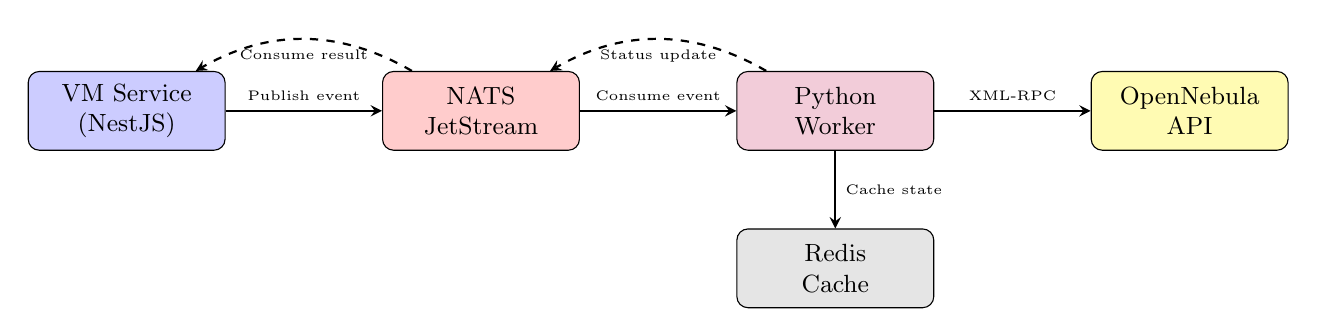
\begin{tikzpicture}[
  box/.style={draw, rounded corners, minimum width=2.5cm, minimum height=1cm, align=center, font=\small},
  arrow/.style={->, thick, >=stealth}
]
  \node[box, fill=blue!20] (vmsvc) at (0, 0) {VM Service\\(NestJS)};
  \node[box, fill=red!20] (nats) at (4.5, 0) {NATS\\JetStream};
  \node[box, fill=purple!20] (worker) at (9, 0) {Python\\Worker};
  \node[box, fill=gray!20] (redis) at (9, -2) {Redis\\Cache};
  \node[box, fill=yellow!30] (one) at (13.5, 0) {OpenNebula\\API};
  
  \draw[arrow] (vmsvc) -- node[above, font=\tiny] {Publish event} (nats);
  \draw[arrow] (nats) -- node[above, font=\tiny] {Consume event} (worker);
  \draw[arrow] (worker) -- node[above, font=\tiny] {XML-RPC} (one);
  \draw[arrow] (worker) -- node[right, font=\tiny] {Cache state} (redis);
  \draw[arrow, dashed] (worker) to[bend right=30] node[below, font=\tiny] {Status update} (nats);
  \draw[arrow, dashed] (nats) to[bend right=30] node[below, font=\tiny] {Consume result} (vmsvc);
\end{tikzpicture}
\caption{Architecture — Worker communication via JetStream}
\label{fig:worker-arch}
\end{figure}

\subsection{Implementation Screenshots}

\begin{figure}[H]
\centering
\fbox{\parbox{0.9\textwidth}{\centering\vspace{3cm}\textit{Insert VM creation form screenshot}\vspace{3cm}}}
\caption{VM creation form}
\label{fig:vm-create-form}
\end{figure}

\begin{figure}[H]
\centering
\fbox{\parbox{0.9\textwidth}{\centering\vspace{3cm}\textit{Insert VM list page screenshot}\vspace{3cm}}}
\caption{VM list page}
\label{fig:vm-list}
\end{figure}

\subsection{Sprint 4 Review}

At the end of Sprint 4:
\begin{itemize}
  \item VM service with full lifecycle operations (create, start, stop, reboot, delete).
  \item Python worker consuming events from NATS JetStream.
  \item Worker communicates with OpenNebula via XML-RPC API.
  \item VM creation form with template selection.
  \item VM list page with status indicators.
  \item OpenNebula virtual networks and storage configured.
  \item End-to-end VM creation working.
\end{itemize}

% ============================================================
\section{Conclusion}

In this chapter, we completed the user management features and the core VM operations. Sprint 3 delivered the admin panel, dashboard layout, and message queue infrastructure. Sprint 4 implemented the central feature of the platform — the ability to create and manage virtual machines through an asynchronous worker that communicates with OpenNebula.

In the next chapter, we will enhance the VM experience with a detailed dashboard, implement the quota system, and build the payment service.

% ============================================================
\chapter{Sprint 3 \& Sprint 4: User Management and VM Operations}

\section{Introduction}

This chapter covers the core features of the platform. Sprint 3 implements user management, the dashboard layout, and NATS JetStream integration. Sprint 4 delivers the central feature — virtual machine lifecycle management through the VM service, Python worker, and OpenNebula integration.

% ============================================================
% SPRINT 3
% ============================================================
\section{Sprint 3: User Management \& Dashboard}

\sprintcard{3}{User Management \& Dashboard}{Implement user CRUD, admin management panel, dashboard layout, and message queue setup.}

\subsection{Sprint Backlog}

\begin{longtable}{|c|p{5cm}|c|c|c|}
\hline
\rowcolor{blue!15}
\textbf{Task ID} & \textbf{Task} & \textbf{Assignee} & \textbf{Est.} & \textbf{Status} \\
\hline
\endhead
T-3.1 & User service CRUD endpoints & DSI & 4h & Done \\
\hline
T-3.2 & Admin user management endpoints & DSI & 3h & Done \\
\hline
T-3.3 & Dashboard layout (sidebar, header) & DSI & 6h & Done \\
\hline
T-3.4 & Profile page (view/edit) & DSI & 4h & Done \\
\hline
T-3.11 & SSH key management (CRUD + UI) & DSI & 5h & Done \\
\hline
T-3.5 & Admin — user list page & DSI & 4h & Done \\
\hline
T-3.6 & NATS JetStream setup & DSI & 4h & Done \\
\hline
T-3.7 & Firewall rules (iptables) & RSI & 6h & Done \\
\hline
T-3.8 & Firewall testing & RSI & 4h & Done \\
\hline
T-3.9 & OpenNebula API access & RSI & 6h & Done \\
\hline
\caption{Sprint 3 backlog}
\label{tab:sprint3-backlog}
\end{longtable}

\subsection{Use Case Diagram — User Management}

\begin{figure}[H]
\centering
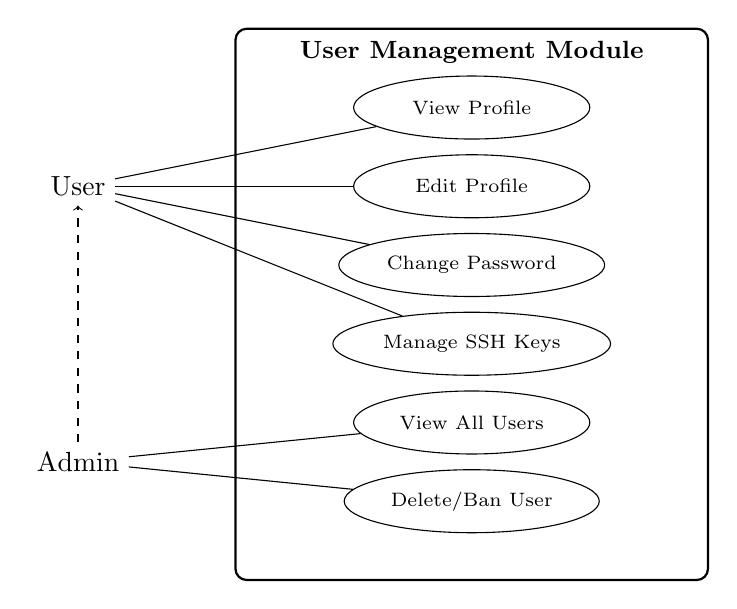
\begin{tikzpicture}[
  usecase/.style={draw, ellipse, minimum width=3cm, minimum height=0.8cm, align=center, font=\scriptsize}
]
  % System boundary
  \draw[thick, rounded corners] (0, -6.5) rectangle (6, 0.5);
  \node[font=\small\bfseries] at (3, 0.2) {User Management Module};
  
  % Actors
  \node (user) at (-2, -1.5) {User};
  \node (admin) at (-2, -5) {Admin};
  
  % Use cases
  \node[usecase] (uc1) at (3, -0.5) {View Profile};
  \node[usecase] (uc2) at (3, -1.5) {Edit Profile};
  \node[usecase] (uc3) at (3, -2.5) {Change Password};
  \node[usecase] (uc6) at (3, -3.5) {Manage SSH Keys};
  \node[usecase] (uc4) at (3, -4.5) {View All Users};
  \node[usecase] (uc5) at (3, -5.5) {Delete/Ban User};
  
  % Arrows
  \draw (user) -- (uc1);
  \draw (user) -- (uc2);
  \draw (user) -- (uc3);
  \draw (user) -- (uc6);
  \draw (admin) -- (uc4);
  \draw (admin) -- (uc5);
  
  % Generalization
  \draw[->, dashed] (admin) -- (user);
  
\end{tikzpicture}
\caption{Use case diagram — User management}
\label{fig:uc-user}
\end{figure}

\subsection{Sequence Diagram — Admin Deletes User}

\begin{figure}[H]
\centering
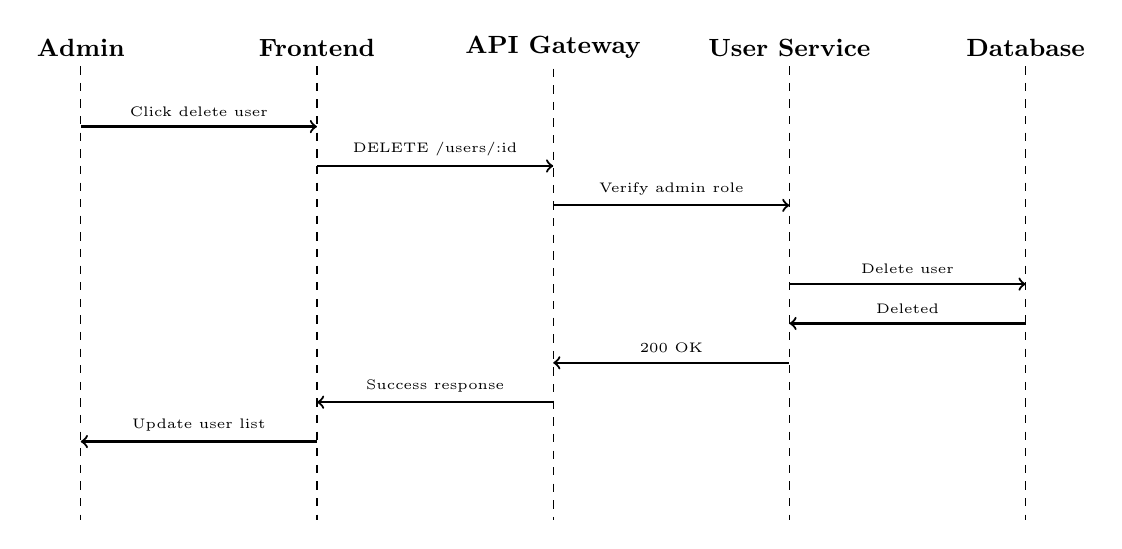
\begin{tikzpicture}[font=\small]
  \node (admin) at (0, 0) {\textbf{Admin}};
  \node (front) at (3, 0) {\textbf{Frontend}};
  \node (gate) at (6, 0) {\textbf{API Gateway}};
  \node (usvc) at (9, 0) {\textbf{User Service}};
  \node (db) at (12, 0) {\textbf{Database}};
  
  \draw[dashed] (admin) -- (0, -6);
  \draw[dashed] (front) -- (3, -6);
  \draw[dashed] (gate) -- (6, -6);
  \draw[dashed] (usvc) -- (9, -6);
  \draw[dashed] (db) -- (12, -6);
  
  \draw[->, thick] (0, -1) -- node[above, font=\tiny] {Click delete user} (3, -1);
  \draw[->, thick] (3, -1.5) -- node[above, font=\tiny] {DELETE /users/:id} (6, -1.5);
  \draw[->, thick] (6, -2) -- node[above, font=\tiny] {Verify admin role} (9, -2);
  \draw[->, thick] (9, -3) -- node[above, font=\tiny] {Delete user} (12, -3);
  \draw[<-, thick] (9, -3.5) -- node[above, font=\tiny] {Deleted} (12, -3.5);
  \draw[<-, thick] (6, -4) -- node[above, font=\tiny] {200 OK} (9, -4);
  \draw[<-, thick] (3, -4.5) -- node[above, font=\tiny] {Success response} (6, -4.5);
  \draw[<-, thick] (0, -5) -- node[above, font=\tiny] {Update user list} (3, -5);
\end{tikzpicture}
\caption{Sequence diagram — Admin deletes user}
\label{fig:seq-delete-user}
\end{figure}

\subsection{Implementation Screenshots}

\begin{figure}[H]
\centering
\fbox{\parbox{0.9\textwidth}{\centering\vspace{3cm}\textit{Insert dashboard layout screenshot}\vspace{3cm}}}
\caption{Dashboard layout with sidebar navigation}
\label{fig:dashboard-layout}
\end{figure}

\begin{figure}[H]
\centering
\fbox{\parbox{0.9\textwidth}{\centering\vspace{3cm}\textit{Insert admin user management screenshot}\vspace{3cm}}}
\caption{Admin — User management page}
\label{fig:admin-users}
\end{figure}

\begin{figure}[H]
\centering
\fbox{\parbox{0.9\textwidth}{\centering\vspace{3cm}\textit{Insert SSH key management page screenshot}\vspace{3cm}}}
\caption{SSH key management — User profile}
\label{fig:ssh-keys}
\end{figure}

\subsection{Sprint 3 Review}

At the end of Sprint 3:
\begin{itemize}
  \item User service with full CRUD operations.
  \item Admin panel for user management.
  \item Dashboard layout with sidebar, header, and responsive design.
  \item Profile page with edit functionality.
  \item SSH key management — users can add, view, and delete SSH public keys.
  \item NATS JetStream configured and tested.
  \item Firewall rules implemented and tested.
  \item OpenNebula XML-RPC API accessible and secured.
\end{itemize}


% ============================================================
% SPRINT 4
% ============================================================
\section{Sprint 4: VM Management \& Worker Service}

\sprintcard{4}{VM Management \& Worker Service}{Implement the core VM lifecycle operations — create, start, stop, reboot, delete — through the web platform with asynchronous processing via the Python worker.}

\subsection{Sprint Backlog}

\begin{longtable}{|c|p{5cm}|c|c|c|}
\hline
\rowcolor{blue!15}
\textbf{Task ID} & \textbf{Task} & \textbf{Assignee} & \textbf{Est.} & \textbf{Status} \\
\hline
\endhead
T-4.1 & VM service — Create VM endpoint & DSI & 5h & Done \\
\hline
T-4.2 & Python worker setup (Redis + NATS) & DSI & 5h & Done \\
\hline
T-4.3 & Worker — Create VM via OpenNebula & DSI & 5h & Done \\
\hline
T-4.4 & Worker — Start/Stop/Reboot ops & DSI & 4h & Done \\
\hline
T-4.5 & Worker — Delete VM operation & DSI & 2h & Done \\
\hline
T-4.6 & VM creation form (frontend) & DSI & 5h & Done \\
\hline
T-4.7 & VM list page (frontend) & DSI & 4h & Done \\
\hline
T-4.8 & OpenNebula API integration testing & RSI & 6h & Done \\
\hline
T-4.9 & VM networking (virtual networks) & RSI & 6h & Done \\
\hline
T-4.10 & Storage + disk images & RSI & 4h & Done \\
\hline
\caption{Sprint 4 backlog}
\label{tab:sprint4-backlog}
\end{longtable}

\subsection{Use Case Diagram — VM Management}

\begin{figure}[H]
\centering
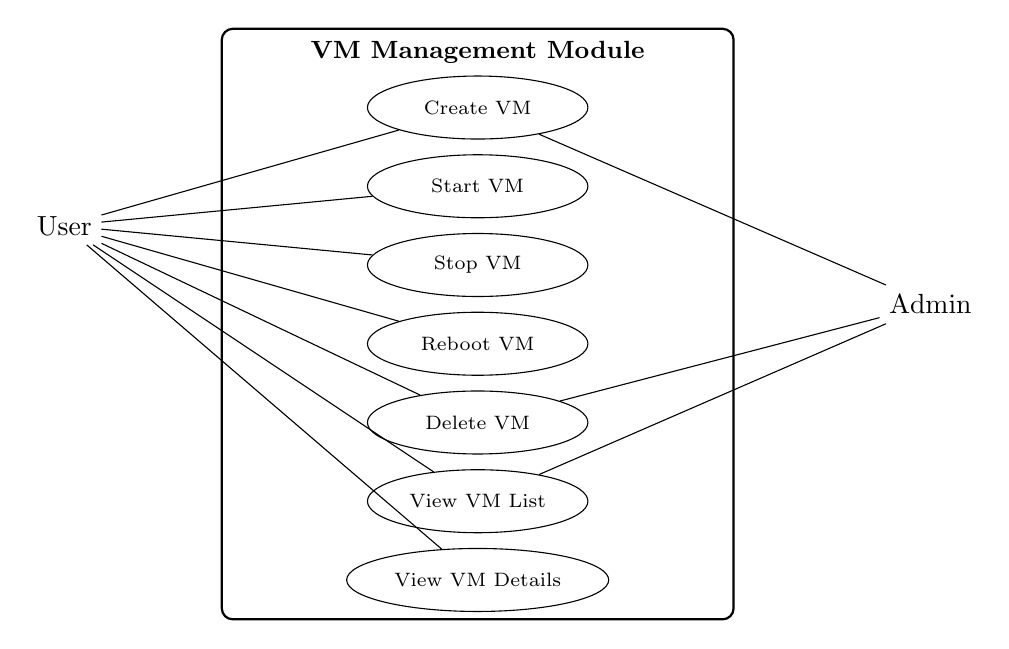
\begin{tikzpicture}[
  usecase/.style={draw, ellipse, minimum width=2.8cm, minimum height=0.8cm, align=center, font=\scriptsize}
]
  % System boundary
  \draw[thick, rounded corners] (0, -7) rectangle (6.5, 0.5);
  \node[font=\small\bfseries] at (3.25, 0.2) {VM Management Module};
  
  % Actors
  \node (user) at (-2, -2) {User};
  \node (admin) at (9, -3) {Admin};
  
  % Use cases
  \node[usecase] (uc1) at (3.25, -0.5) {Create VM};
  \node[usecase] (uc2) at (3.25, -1.5) {Start VM};
  \node[usecase] (uc3) at (3.25, -2.5) {Stop VM};
  \node[usecase] (uc4) at (3.25, -3.5) {Reboot VM};
  \node[usecase] (uc5) at (3.25, -4.5) {Delete VM};
  \node[usecase] (uc6) at (3.25, -5.5) {View VM List};
  \node[usecase] (uc7) at (3.25, -6.5) {View VM Details};
  
  % Arrows
  \draw (user) -- (uc1);
  \draw (user) -- (uc2);
  \draw (user) -- (uc3);
  \draw (user) -- (uc4);
  \draw (user) -- (uc5);
  \draw (user) -- (uc6);
  \draw (user) -- (uc7);
  
  \draw (admin) -- (uc1);
  \draw (admin) -- (uc5);
  \draw (admin) -- (uc6);
  
\end{tikzpicture}
\caption{Use case diagram — VM management}
\label{fig:uc-vm}
\end{figure}

\subsection{Sequence Diagram — VM Creation (End-to-End)}

\begin{figure}[H]
\centering
\begin{tikzpicture}[font=\scriptsize]
  % Lifelines
  \node (user) at (0, 0) {\textbf{User}};
  \node (front) at (2, 0) {\textbf{Frontend}};
  \node (gate) at (4, 0) {\textbf{Gateway}};
  \node (vmsvc) at (6, 0) {\textbf{VM Service}};
  \node (nats) at (8, 0) {\textbf{JetStream}};
  \node (worker) at (10, 0) {\textbf{Worker}};
  \node (one) at (12.5, 0) {\textbf{OpenNebula}};
  
  \draw[dashed] (user) -- (0, -11);
  \draw[dashed] (front) -- (2, -11);
  \draw[dashed] (gate) -- (4, -11);
  \draw[dashed] (vmsvc) -- (6, -11);
  \draw[dashed] (nats) -- (8, -11);
  \draw[dashed] (worker) -- (10, -11);
  \draw[dashed] (one) -- (12.5, -11);
  
  % Messages
  \draw[->, thick] (0, -0.8) -- node[above] {Fill VM form} (2, -0.8);
  \draw[->, thick] (2, -1.5) -- node[above] {POST /vms} (4, -1.5);
  \draw[->, thick] (4, -2.2) -- node[above] {Forward} (6, -2.2);
  \draw[->, thick] (6, -2.7) -- node[right] {Check quota};
  \draw[->, thick] (6, -3.5) -- node[above] {Save VM (pending)} (6, -3.5);
  \draw[->, thick] (6, -4.2) -- node[above] {Publish event} (8, -4.2);
  \draw[<-, thick] (4, -4.9) -- node[above] {202 Accepted} (6, -4.9);
  \draw[<-, thick] (2, -5.3) -- node[above] {VM creating...} (4, -5.3);
  \draw[->, thick] (8, -6) -- node[above] {Consume event} (10, -6);
  \draw[->, thick] (10, -6.7) -- node[above] {Create VM} (12.5, -6.7);
  \draw[<-, thick] (10, -7.4) -- node[above] {VM ID + IP} (12.5, -7.4);
  \draw[->, thick] (10, -8.1) -- node[above] {Publish result} (8, -8.1);
  \draw[->, thick] (6, -8.8) -- node[above] {Update status} (6, -8.8);
  \draw[->, thick] (6, -9) -- node[right] {VM → running};
  \draw[<-, thick] (2, -9.7) -- node[above] {Status update} (6, -9.7);
  \draw[<-, thick] (0, -10.3) -- node[above] {VM ready!} (2, -10.3);
\end{tikzpicture}
\caption{Sequence diagram — VM creation (end-to-end)}
\label{fig:seq-vm-create}
\end{figure}

\subsection{Activity Diagram — VM Lifecycle}

\begin{figure}[H]
\centering
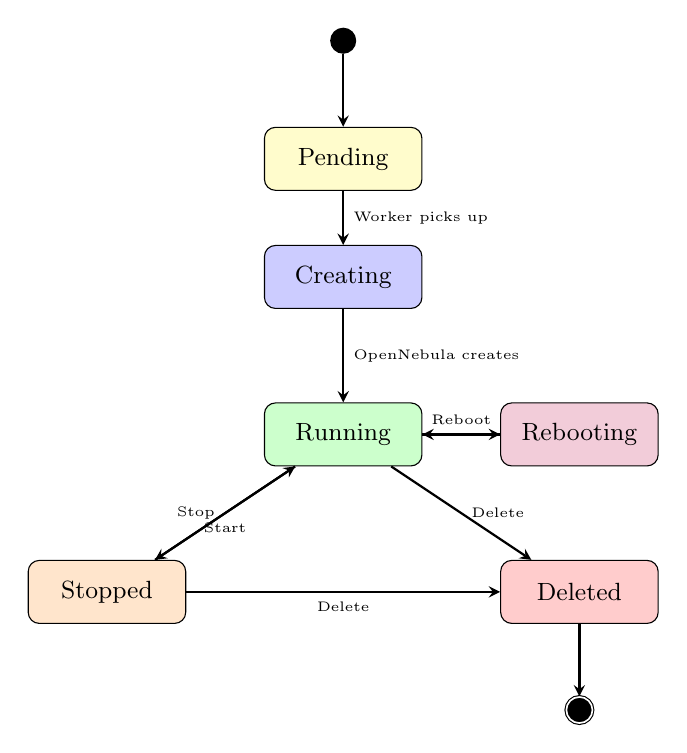
\begin{tikzpicture}[
  state/.style={draw, rounded corners, minimum width=2cm, minimum height=0.8cm, align=center, font=\small},
  decision/.style={draw, diamond, minimum width=1.5cm, minimum height=1cm, align=center, font=\tiny},
  arrow/.style={->, thick, >=stealth}
]
  % States
  \node[circle, fill=black, minimum size=0.3cm] (start) at (0, 0) {};
  \node[state, fill=yellow!20] (pending) at (0, -1.5) {Pending};
  \node[state, fill=blue!20] (creating) at (0, -3) {Creating};
  \node[state, fill=green!20] (running) at (0, -5) {Running};
  \node[state, fill=orange!20] (stopped) at (-3, -7) {Stopped};
  \node[state, fill=red!20] (deleted) at (3, -7) {Deleted};
  \node[state, fill=purple!20] (rebooting) at (3, -5) {Rebooting};
  \node[circle, draw, fill=black, minimum size=0.3cm, double] (end) at (3, -8.5) {};
  
  % Arrows
  \draw[arrow] (start) -- (pending);
  \draw[arrow] (pending) -- node[right, font=\tiny] {Worker picks up} (creating);
  \draw[arrow] (creating) -- node[right, font=\tiny] {OpenNebula creates} (running);
  \draw[arrow] (running) -- node[left, font=\tiny] {Stop} (stopped);
  \draw[arrow] (stopped) -- node[below, font=\tiny] {Start} (running);
  \draw[arrow] (running) -- node[above, font=\tiny] {Reboot} (rebooting);
  \draw[arrow] (rebooting) -- node[right, font=\tiny] {} (running);
  \draw[arrow] (running) -- node[right, font=\tiny] {Delete} (deleted);
  \draw[arrow] (stopped) -- node[below, font=\tiny] {Delete} (deleted);
  \draw[arrow] (deleted) -- (end);
\end{tikzpicture}
\caption{Activity diagram — VM lifecycle}
\label{fig:activity-vm}
\end{figure}

\subsection{Class Diagram — VM Module}

\begin{figure}[H]
\centering
\begin{tikzpicture}[font=\small,
  class/.style={draw, rectangle, minimum width=4cm, align=left}
]
  % VM class
  \node[class, fill=yellow!15] (vmclass) at (0, 0) {
    \textbf{VirtualMachine}\\
    \hline
    - id: UUID\\
    - name: String\\
    - userId: UUID\\
    - templateId: String\\
    - vcpu: Integer\\
    - ram: Integer (MB)\\
    - disk: Integer (GB)\\
    - status: VMStatus\\
    - ipAddress: String\\
    - oneId: Integer\\
    - createdAt: DateTime\\
    \hline
    + create()\\
    + start()\\
    + stop()\\
    + reboot()\\
    + delete()
  };
  
  % VMStatus enum
  \node[class, fill=green!15] (statusenum) at (6, 1) {
    \textbf{<<enum>> VMStatus}\\
    \hline
    PENDING\\
    CREATING\\
    RUNNING\\
    STOPPED\\
    REBOOTING\\
    DELETING\\
    DELETED\\
    ERROR
  };
  
  % VMTemplate
  \node[class, fill=blue!15] (template) at (6, -3.5) {
    \textbf{VMTemplate}\\
    \hline
    - id: String\\
    - name: String\\
    - os: String\\
    - minCpu: Integer\\
    - minRam: Integer\\
    - minDisk: Integer\\
    \hline
    + getTemplates()
  };
  
  % Relations
  \draw[->, thick] (vmclass) -- node[above, font=\tiny] {has} (statusenum);
  \draw[->, thick] (vmclass) -- node[below, font=\tiny] {uses} (template);
\end{tikzpicture}
\caption{Class diagram — VM module}
\label{fig:class-vm}
\end{figure}

\subsection{Architecture Diagram — Worker Communication}

\begin{figure}[H]
\centering
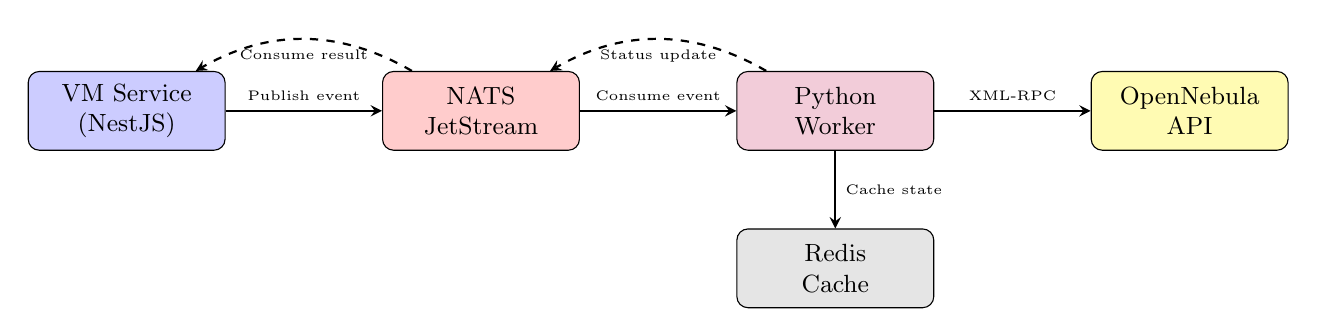
\begin{tikzpicture}[
  box/.style={draw, rounded corners, minimum width=2.5cm, minimum height=1cm, align=center, font=\small},
  arrow/.style={->, thick, >=stealth}
]
  \node[box, fill=blue!20] (vmsvc) at (0, 0) {VM Service\\(NestJS)};
  \node[box, fill=red!20] (nats) at (4.5, 0) {NATS\\JetStream};
  \node[box, fill=purple!20] (worker) at (9, 0) {Python\\Worker};
  \node[box, fill=gray!20] (redis) at (9, -2) {Redis\\Cache};
  \node[box, fill=yellow!30] (one) at (13.5, 0) {OpenNebula\\API};
  
  \draw[arrow] (vmsvc) -- node[above, font=\tiny] {Publish event} (nats);
  \draw[arrow] (nats) -- node[above, font=\tiny] {Consume event} (worker);
  \draw[arrow] (worker) -- node[above, font=\tiny] {XML-RPC} (one);
  \draw[arrow] (worker) -- node[right, font=\tiny] {Cache state} (redis);
  \draw[arrow, dashed] (worker) to[bend right=30] node[below, font=\tiny] {Status update} (nats);
  \draw[arrow, dashed] (nats) to[bend right=30] node[below, font=\tiny] {Consume result} (vmsvc);
\end{tikzpicture}
\caption{Architecture — Worker communication via JetStream}
\label{fig:worker-arch}
\end{figure}

\subsection{Implementation Screenshots}

\begin{figure}[H]
\centering
\fbox{\parbox{0.9\textwidth}{\centering\vspace{3cm}\textit{Insert VM creation form screenshot}\vspace{3cm}}}
\caption{VM creation form}
\label{fig:vm-create-form}
\end{figure}

\begin{figure}[H]
\centering
\fbox{\parbox{0.9\textwidth}{\centering\vspace{3cm}\textit{Insert VM list page screenshot}\vspace{3cm}}}
\caption{VM list page}
\label{fig:vm-list}
\end{figure}

\subsection{Sprint 4 Review}

At the end of Sprint 4:
\begin{itemize}
  \item VM service with full lifecycle operations (create, start, stop, reboot, delete).
  \item Python worker consuming events from NATS JetStream.
  \item Worker communicates with OpenNebula via XML-RPC API.
  \item VM creation form with template selection.
  \item VM list page with status indicators.
  \item OpenNebula virtual networks and storage configured.
  \item End-to-end VM creation working.
\end{itemize}

% ============================================================
\section{Conclusion}

In this chapter, we completed the user management features and the core VM operations. Sprint 3 delivered the admin panel, dashboard layout, and message queue infrastructure. Sprint 4 implemented the central feature of the platform — the ability to create and manage virtual machines through an asynchronous worker that communicates with OpenNebula.

In the next chapter, we will enhance the VM experience with a detailed dashboard, implement the quota system, and build the payment service.


% ============================================================
% CHAPTER 4: Sprint 5 & 6 (Quotas + Payments)
% ============================================================
% % ============================================================
% CHAPTER 4: Sprint 5 & Sprint 6 — Quotas & Payments
% ============================================================
% ADD THIS TO main.tex AFTER COMPLETING SPRINT 5 & 6
% Uncomment: % ============================================================
% CHAPTER 4: Sprint 5 & Sprint 6 — Quotas & Payments
% ============================================================
% ADD THIS TO main.tex AFTER COMPLETING SPRINT 5 & 6
% Uncomment: % ============================================================
% CHAPTER 4: Sprint 5 & Sprint 6 — Quotas & Payments
% ============================================================
% ADD THIS TO main.tex AFTER COMPLETING SPRINT 5 & 6
% Uncomment: \input{chapters/chapter4}
% ============================================================
\chapter{Sprint 5 \& Sprint 6: Quotas and Payment Service}

\section{Introduction}

This chapter covers the business logic layer of the platform. Sprint 5 implements the VM dashboard with detailed information and the quota system that enforces resource limits per user. Sprint 6 delivers the payment service with plan management and upgrade flows.

% ============================================================
% SPRINT 5
% ============================================================
\section{Sprint 5: VM Dashboard \& Quota System}

\sprintcard{5}{VM Dashboard \& Quota System}{Deliver a comprehensive VM dashboard with status monitoring, and implement quota enforcement to limit resource usage per plan.}

\subsection{Sprint Backlog}

\begin{longtable}{|c|p{5cm}|c|c|c|}
\hline
\rowcolor{blue!15}
\textbf{Task ID} & \textbf{Task} & \textbf{Assignee} & \textbf{Est.} & \textbf{Status} \\
\hline
\endhead
T-5.1 & VM detail page (frontend) & DSI & 5h & Done \\
\hline
T-5.10 & Web terminal (xterm.js + WebSocket SSH) & DSI & 6h & Done \\
\hline
T-5.2 & VM action buttons + confirmation & DSI & 4h & Done \\
\hline
T-5.3 & Quota tracking implementation & DSI & 4h & Done \\
\hline
T-5.4 & Quota enforcement on VM creation & DSI & 3h & Done \\
\hline
T-5.5 & Admin VM management page & DSI & 5h & Done \\
\hline
T-5.6 & Quota display on dashboard & DSI & 3h & Done \\
\hline
T-5.7 & Server monitoring setup & RSI & 6h & Done \\
\hline
T-5.8 & Backup procedures & RSI & 4h & Done \\
\hline
T-5.9 & Network security audit & RSI & 4h & Done \\
\hline
\caption{Sprint 5 backlog}
\label{tab:sprint5-backlog}
\end{longtable}

\subsection{Use Case Diagram — Quota Management}

\begin{figure}[H]
\centering
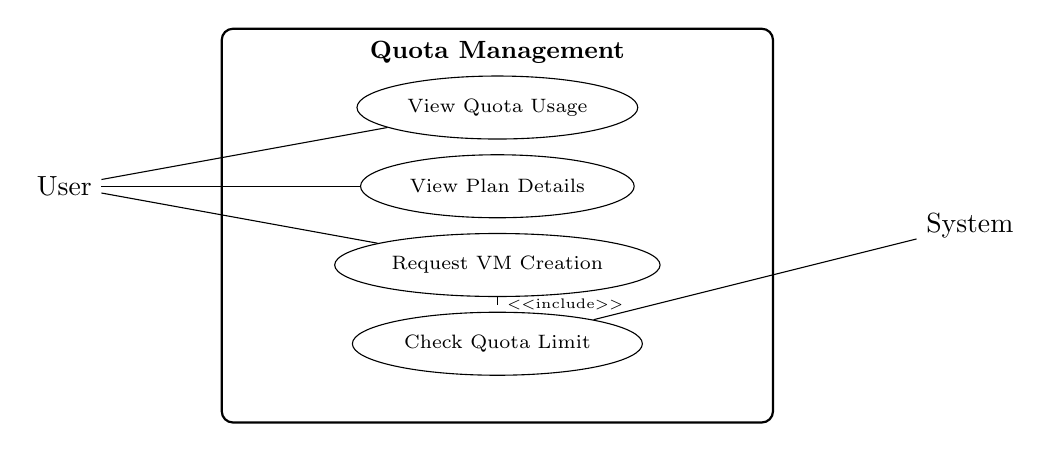
\begin{tikzpicture}[
  usecase/.style={draw, ellipse, minimum width=3cm, minimum height=0.8cm, align=center, font=\scriptsize}
]
  \draw[thick, rounded corners] (0, -4.5) rectangle (7, 0.5);
  \node[font=\small\bfseries] at (3.5, 0.2) {Quota Management};
  
  \node (user) at (-2, -1.5) {User};
  \node (system) at (9.5, -2) {System};
  
  \node[usecase] (uc1) at (3.5, -0.5) {View Quota Usage};
  \node[usecase] (uc2) at (3.5, -1.5) {View Plan Details};
  \node[usecase] (uc3) at (3.5, -2.5) {Request VM Creation};
  \node[usecase] (uc4) at (3.5, -3.5) {Check Quota Limit};
  
  \draw (user) -- (uc1);
  \draw (user) -- (uc2);
  \draw (user) -- (uc3);
  \draw[dashed] (uc3) -- node[right, font=\tiny] {<<include>>} (uc4);
  \draw (system) -- (uc4);
\end{tikzpicture}
\caption{Use case diagram — Quota management}
\label{fig:uc-quota}
\end{figure}

\subsection{Sequence Diagram — Quota Check on VM Creation}

\begin{figure}[H]
\centering
\begin{tikzpicture}[font=\small]
  \node (user) at (0, 0) {\textbf{User}};
  \node (vmsvc) at (4, 0) {\textbf{VM Service}};
  \node (quota) at (8, 0) {\textbf{Quota Service}};
  \node (db) at (12, 0) {\textbf{Database}};
  
  \draw[dashed] (user) -- (0, -8);
  \draw[dashed] (vmsvc) -- (4, -8);
  \draw[dashed] (quota) -- (8, -8);
  \draw[dashed] (db) -- (12, -8);
  
  \draw[->, thick] (0, -1) -- node[above, font=\tiny] {Create VM request} (4, -1);
  \draw[->, thick] (4, -2) -- node[above, font=\tiny] {Check user quota} (8, -2);
  \draw[->, thick] (8, -3) -- node[above, font=\tiny] {Get user plan + VM count} (12, -3);
  \draw[<-, thick] (8, -3.5) -- node[above, font=\tiny] {Plan: Pro, VMs: 3/5} (12, -3.5);
  \draw[<-, thick] (4, -4.5) -- node[above, font=\tiny] {Quota OK (3 < 5)} (8, -4.5);
  \draw[->, thick] (4, -5.5) -- node[right, font=\tiny] {Proceed with creation};
  
  % Alternative (quota exceeded)
  \draw[thick, red, dashed] (1, -6) rectangle (11, -7.5);
  \node[red, font=\tiny] at (6, -6.3) {alt: Quota Exceeded};
  \draw[->, thick, red] (8, -7) -- node[above, font=\tiny, red] {403 Quota Exceeded} (4, -7);
\end{tikzpicture}
\caption{Sequence diagram — Quota check on VM creation}
\label{fig:seq-quota}
\end{figure}

\subsection{Class Diagram — Quota \& Plan}

\begin{figure}[H]
\centering
\begin{tikzpicture}[font=\small,
  class/.style={draw, rectangle, minimum width=3.5cm, align=left}
]
  \node[class, fill=yellow!15] (plan) at (0, 0) {
    \textbf{Plan}\\
    \hline
    - id: UUID\\
    - name: String\\
    - maxVMs: Integer\\
    - maxCPU: Integer\\
    - maxRAM: Integer\\
    - maxDisk: Integer\\
    - price: Decimal\\
    \hline
    + getPlans()
  };
  
  \node[class, fill=blue!15] (quota) at (6, 0) {
    \textbf{UserQuota}\\
    \hline
    - id: UUID\\
    - userId: UUID\\
    - planId: UUID\\
    - usedVMs: Integer\\
    - usedCPU: Integer\\
    - usedRAM: Integer\\
    - usedDisk: Integer\\
    \hline
    + checkLimit()\\
    + updateUsage()
  };
  
  \draw[->, thick] (quota) -- node[above, font=\tiny] {belongs to} (plan);
\end{tikzpicture}
\caption{Class diagram — Plan and quota}
\label{fig:class-quota}
\end{figure}

\subsection{Implementation Screenshots}

\begin{figure}[H]
\centering
\fbox{\parbox{0.9\textwidth}{\centering\vspace{3cm}\textit{Insert VM detail page screenshot}\vspace{3cm}}}
\caption{VM detail page with status, IP, and resources}
\label{fig:vm-detail}
\end{figure}

\begin{figure}[H]
\centering
\fbox{\parbox{0.9\textwidth}{\centering\vspace{3cm}\textit{Insert quota usage display screenshot}\vspace{3cm}}}
\caption{Dashboard — Quota usage display}
\label{fig:quota-display}
\end{figure}
\subsection{Sequence Diagram --- Web Terminal Connection}

\begin{figure}[H]
\centering
\begin{tikzpicture}[font=\small]
  \node (user) at (0, 0) {\textbf{User}};
  \node (front) at (3, 0) {\textbf{Frontend}};
  \node (gate) at (6, 0) {\textbf{Gateway}};
  \node (proxy) at (9, 0) {\textbf{SSH Proxy}};
  \node (vm) at (12, 0) {\textbf{VM (SSH)}};
  
  \draw[dashed] (user) -- (0, -9);
  \draw[dashed] (front) -- (3, -9);
  \draw[dashed] (gate) -- (6, -9);
  \draw[dashed] (proxy) -- (9, -9);
  \draw[dashed] (vm) -- (12, -9);
  
  \draw[->, thick] (0, -0.8) -- node[above, font=\tiny] {Click ``Terminal''} (3, -0.8);
  \draw[->, thick] (3, -1.5) -- node[above, font=\tiny] {WebSocket connect} (6, -1.5);
  \draw[->, thick] (6, -2.2) -- node[above, font=\tiny] {Get user SSH key} (6, -2.2);
  \draw[->, thick] (6, -2.7) -- node[right, font=\tiny] {Verify JWT};
  \draw[->, thick] (6, -3.5) -- node[above, font=\tiny] {Open SSH tunnel} (9, -3.5);
  \draw[->, thick] (9, -4.2) -- node[above, font=\tiny] {SSH connect (key auth)} (12, -4.2);
  \draw[<-, thick] (9, -4.9) -- node[above, font=\tiny] {Shell session open} (12, -4.9);
  \draw[<-, thick] (6, -5.6) -- node[above, font=\tiny] {Tunnel ready} (9, -5.6);
  \draw[<-, thick] (3, -6.3) -- node[above, font=\tiny] {WS connected} (6, -6.3);
  \draw[->, thick] (3, -7) -- node[below, font=\tiny] {xterm.js renders terminal} (3, -7);
  \draw[<->, thick] (0, -7.5) -- node[above, font=\tiny] {Type commands / see output} (3, -7.5);
  \draw[<->, thick, blue, dashed] (3, -8.2) -- node[above, font=\tiny, blue] {Bidirectional data stream} (12, -8.2);
\end{tikzpicture}
\caption{Sequence diagram --- Web terminal connection (Phase~1)}
\label{fig:seq-terminal}
\end{figure}

\begin{figure}[H]
\centering
\fbox{\parbox{0.9\textwidth}{\centering\vspace{3cm}\textit{Insert web terminal (CLI) screenshot --- user accessing VM from browser}\vspace{3cm}}}
\caption{Web terminal --- CLI access to VM via xterm.js (Phase~1)}
\label{fig:web-terminal}
\end{figure}
\subsection{Sprint 5 Review}

At the end of Sprint 5:
\begin{itemize}
  \item VM detail page showing IP, status, OS, CPU, RAM, uptime.
  \item \textbf{Web terminal (Phase~1)} --- users can access VMs via a CLI terminal in the browser using xterm.js and WebSocket SSH proxy.
  \item VM action buttons (start, stop, reboot, delete) with confirmation dialogs.
  \item Quota system tracking and enforcing resource limits.
  \item Admin VM management page with filtering.
  \item Server monitoring and backup procedures in place.
\end{itemize}


% ============================================================
% SPRINT 6
% ============================================================
\section{Sprint 6: Payment Service}

\sprintcard{6}{Payment Service}{Implement payment processing with plan management, upgrade flows, and billing history.}

\subsection{Sprint Backlog}

\begin{longtable}{|c|p{5cm}|c|c|c|}
\hline
\rowcolor{blue!15}
\textbf{Task ID} & \textbf{Task} & \textbf{Assignee} & \textbf{Est.} & \textbf{Status} \\
\hline
\endhead
T-6.1 & Plans CRUD (backend) & DSI & 4h & Done \\
\hline
T-6.2 & Payment processing (Stripe/mock) & DSI & 5h & Done \\
\hline
T-6.3 & Billing page (frontend) & DSI & 4h & Done \\
\hline
T-6.4 & Checkout flow (frontend) & DSI & 5h & Done \\
\hline
T-6.5 & Payment history page & DSI & 3h & Done \\
\hline
T-6.6 & Admin plan management page & DSI & 3h & Done \\
\hline
T-6.7 & SSL/TLS configuration & RSI & 4h & Done \\
\hline
T-6.8 & Log management & RSI & 4h & Done \\
\hline
T-6.9 & OpenNebula optimization & RSI & 4h & Done \\
\hline
\caption{Sprint 6 backlog}
\label{tab:sprint6-backlog}
\end{longtable}

\subsection{Use Case Diagram — Payment}

\begin{figure}[H]
\centering
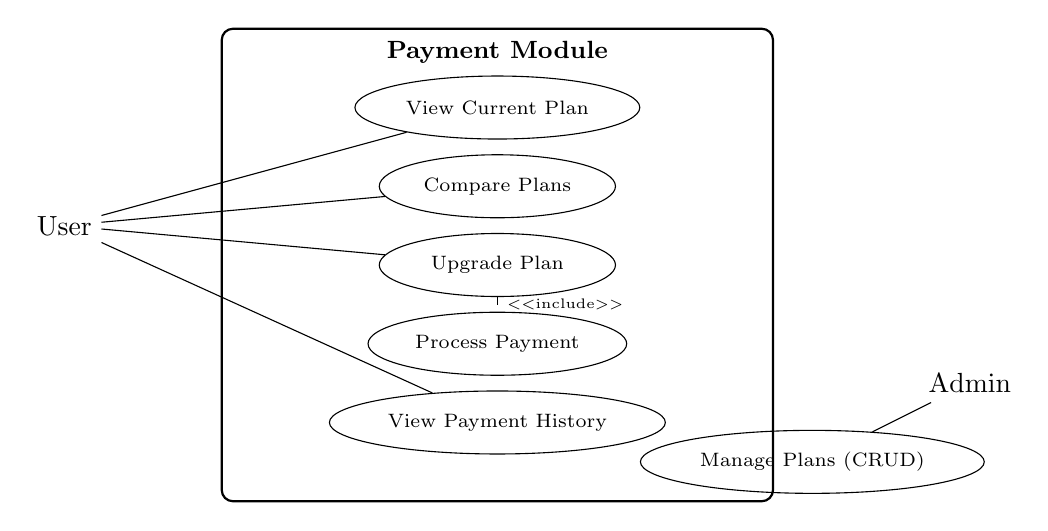
\begin{tikzpicture}[
  usecase/.style={draw, ellipse, minimum width=3cm, minimum height=0.8cm, align=center, font=\scriptsize}
]
  \draw[thick, rounded corners] (0, -5.5) rectangle (7, 0.5);
  \node[font=\small\bfseries] at (3.5, 0.2) {Payment Module};
  
  \node (user) at (-2, -2) {User};
  \node (admin) at (9.5, -4) {Admin};
  
  \node[usecase] (uc1) at (3.5, -0.5) {View Current Plan};
  \node[usecase] (uc2) at (3.5, -1.5) {Compare Plans};
  \node[usecase] (uc3) at (3.5, -2.5) {Upgrade Plan};
  \node[usecase] (uc4) at (3.5, -3.5) {Process Payment};
  \node[usecase] (uc5) at (3.5, -4.5) {View Payment History};
  
  \draw (user) -- (uc1);
  \draw (user) -- (uc2);
  \draw (user) -- (uc3);
  \draw (user) -- (uc5);
  \draw[dashed] (uc3) -- node[right, font=\tiny] {<<include>>} (uc4);
  
  \node[usecase] (uc6) at (7.5, -5) {Manage Plans (CRUD)};
  \draw (admin) -- (uc6);
\end{tikzpicture}
\caption{Use case diagram — Payment module}
\label{fig:uc-payment}
\end{figure}

\subsection{Sequence Diagram — Plan Upgrade}

\begin{figure}[H]
\centering
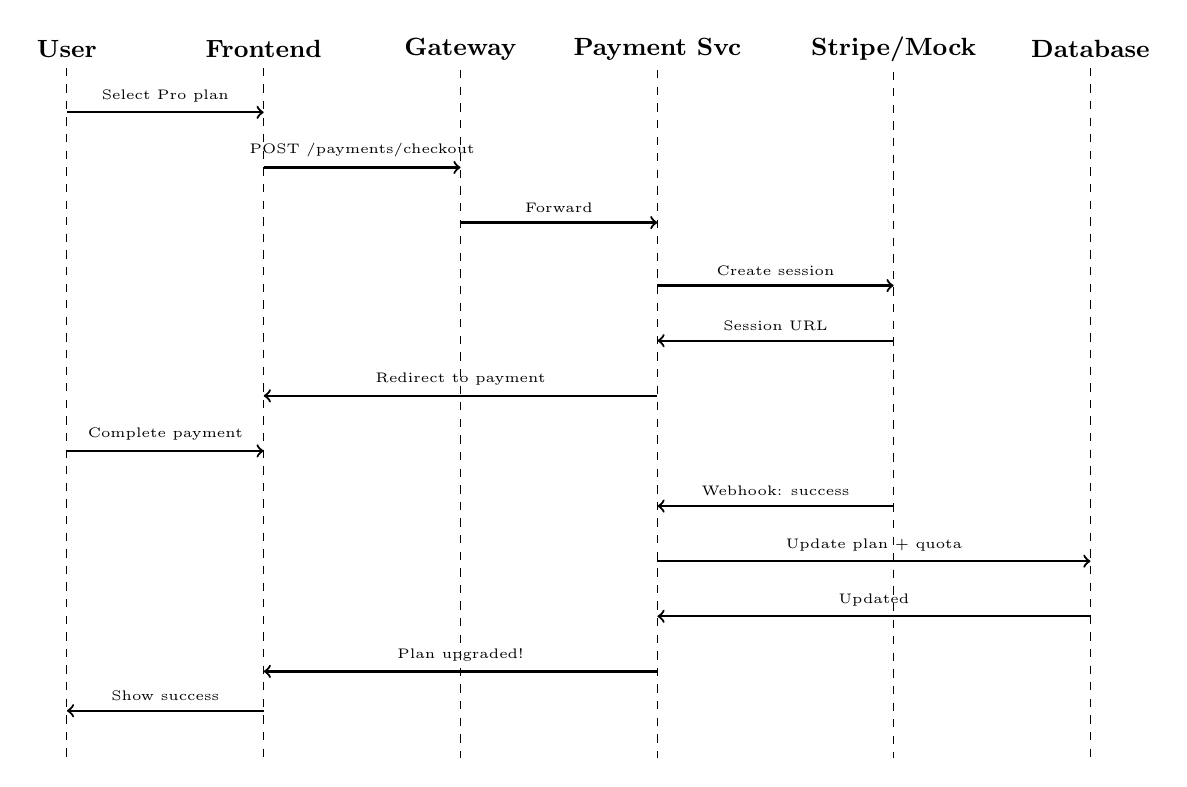
\begin{tikzpicture}[font=\small]
  \node (user) at (0, 0) {\textbf{User}};
  \node (front) at (2.5, 0) {\textbf{Frontend}};
  \node (gate) at (5, 0) {\textbf{Gateway}};
  \node (pay) at (7.5, 0) {\textbf{Payment Svc}};
  \node (stripe) at (10.5, 0) {\textbf{Stripe/Mock}};
  \node (db) at (13, 0) {\textbf{Database}};
  
  \draw[dashed] (user) -- (0, -9);
  \draw[dashed] (front) -- (2.5, -9);
  \draw[dashed] (gate) -- (5, -9);
  \draw[dashed] (pay) -- (7.5, -9);
  \draw[dashed] (stripe) -- (10.5, -9);
  \draw[dashed] (db) -- (13, -9);
  
  \draw[->, thick] (0, -0.8) -- node[above, font=\tiny] {Select Pro plan} (2.5, -0.8);
  \draw[->, thick] (2.5, -1.5) -- node[above, font=\tiny] {POST /payments/checkout} (5, -1.5);
  \draw[->, thick] (5, -2.2) -- node[above, font=\tiny] {Forward} (7.5, -2.2);
  \draw[->, thick] (7.5, -3) -- node[above, font=\tiny] {Create session} (10.5, -3);
  \draw[<-, thick] (7.5, -3.7) -- node[above, font=\tiny] {Session URL} (10.5, -3.7);
  \draw[<-, thick] (2.5, -4.4) -- node[above, font=\tiny] {Redirect to payment} (7.5, -4.4);
  \draw[->, thick] (0, -5.1) -- node[above, font=\tiny] {Complete payment} (2.5, -5.1);
  \draw[->, thick] (10.5, -5.8) -- node[above, font=\tiny] {Webhook: success} (7.5, -5.8);
  \draw[->, thick] (7.5, -6.5) -- node[above, font=\tiny] {Update plan + quota} (13, -6.5);
  \draw[<-, thick] (7.5, -7.2) -- node[above, font=\tiny] {Updated} (13, -7.2);
  \draw[<-, thick] (2.5, -7.9) -- node[above, font=\tiny] {Plan upgraded!} (7.5, -7.9);
  \draw[<-, thick] (0, -8.4) -- node[above, font=\tiny] {Show success} (2.5, -8.4);
\end{tikzpicture}
\caption{Sequence diagram — Plan upgrade with payment}
\label{fig:seq-payment}
\end{figure}

\subsection{Class Diagram — Payment Module}

\begin{figure}[H]
\centering
\begin{tikzpicture}[font=\small,
  class/.style={draw, rectangle, minimum width=3.5cm, align=left}
]
  \node[class, fill=yellow!15] (payment) at (0, 0) {
    \textbf{Payment}\\
    \hline
    - id: UUID\\
    - userId: UUID\\
    - planId: UUID\\
    - amount: Decimal\\
    - currency: String\\
    - status: PaymentStatus\\
    - stripeSessionId: String\\
    - createdAt: DateTime\\
    \hline
    + createCheckout()\\
    + processWebhook()
  };
  
  \node[class, fill=green!15] (pstatus) at (6, 0) {
    \textbf{<<enum>> PaymentStatus}\\
    \hline
    PENDING\\
    COMPLETED\\
    FAILED\\
    REFUNDED
  };
  
  \node[class, fill=blue!15] (invoice) at (0, -4.5) {
    \textbf{Invoice}\\
    \hline
    - id: UUID\\
    - paymentId: UUID\\
    - invoiceNumber: String\\
    - pdfUrl: String\\
    - createdAt: DateTime\\
    \hline
    + generate()
  };
  
  \draw[->, thick] (payment) -- (pstatus);
  \draw[->, thick] (payment) -- node[left, font=\tiny] {generates} (invoice);
\end{tikzpicture}
\caption{Class diagram — Payment module}
\label{fig:class-payment}
\end{figure}

\subsection{Implementation Screenshots}

\begin{figure}[H]
\centering
\fbox{\parbox{0.9\textwidth}{\centering\vspace{3cm}\textit{Insert billing page screenshot}\vspace{3cm}}}
\caption{Billing page — Current plan and usage}
\label{fig:billing-page}
\end{figure}

\begin{figure}[H]
\centering
\fbox{\parbox{0.9\textwidth}{\centering\vspace{3cm}\textit{Insert checkout flow screenshot}\vspace{3cm}}}
\caption{Checkout flow — Plan upgrade}
\label{fig:checkout}
\end{figure}

\begin{figure}[H]
\centering
\fbox{\parbox{0.9\textwidth}{\centering\vspace{3cm}\textit{Insert payment history screenshot}\vspace{3cm}}}
\caption{Payment history page}
\label{fig:payment-history}
\end{figure}

\subsection{Sprint 6 Review}

At the end of Sprint 6:
\begin{itemize}
  \item Payment service with plan CRUD and checkout.
  \item Stripe/mock payment processing with webhooks.
  \item Billing page displaying current plan and usage.
  \item Checkout flow for plan upgrades.
  \item Payment history with transaction records.
  \item Admin plan management page.
  \item SSL/TLS configured on the server.
\end{itemize}

% ============================================================
\section{Conclusion}

This chapter delivered the business layer of the platform. Sprint 5 enhanced the VM experience with detailed monitoring, \textbf{web-based CLI terminal access (Phase~1)}, and enforced resource limits through the quota system. Sprint 6 completed the monetization aspect with a full payment service supporting plan upgrades and billing history.

In the next chapter, we will finalize the platform with notifications, comprehensive testing, deployment, and project documentation.

% ============================================================
\chapter{Sprint 5 \& Sprint 6: Quotas and Payment Service}

\section{Introduction}

This chapter covers the business logic layer of the platform. Sprint 5 implements the VM dashboard with detailed information and the quota system that enforces resource limits per user. Sprint 6 delivers the payment service with plan management and upgrade flows.

% ============================================================
% SPRINT 5
% ============================================================
\section{Sprint 5: VM Dashboard \& Quota System}

\sprintcard{5}{VM Dashboard \& Quota System}{Deliver a comprehensive VM dashboard with status monitoring, and implement quota enforcement to limit resource usage per plan.}

\subsection{Sprint Backlog}

\begin{longtable}{|c|p{5cm}|c|c|c|}
\hline
\rowcolor{blue!15}
\textbf{Task ID} & \textbf{Task} & \textbf{Assignee} & \textbf{Est.} & \textbf{Status} \\
\hline
\endhead
T-5.1 & VM detail page (frontend) & DSI & 5h & Done \\
\hline
T-5.10 & Web terminal (xterm.js + WebSocket SSH) & DSI & 6h & Done \\
\hline
T-5.2 & VM action buttons + confirmation & DSI & 4h & Done \\
\hline
T-5.3 & Quota tracking implementation & DSI & 4h & Done \\
\hline
T-5.4 & Quota enforcement on VM creation & DSI & 3h & Done \\
\hline
T-5.5 & Admin VM management page & DSI & 5h & Done \\
\hline
T-5.6 & Quota display on dashboard & DSI & 3h & Done \\
\hline
T-5.7 & Server monitoring setup & RSI & 6h & Done \\
\hline
T-5.8 & Backup procedures & RSI & 4h & Done \\
\hline
T-5.9 & Network security audit & RSI & 4h & Done \\
\hline
\caption{Sprint 5 backlog}
\label{tab:sprint5-backlog}
\end{longtable}

\subsection{Use Case Diagram — Quota Management}

\begin{figure}[H]
\centering
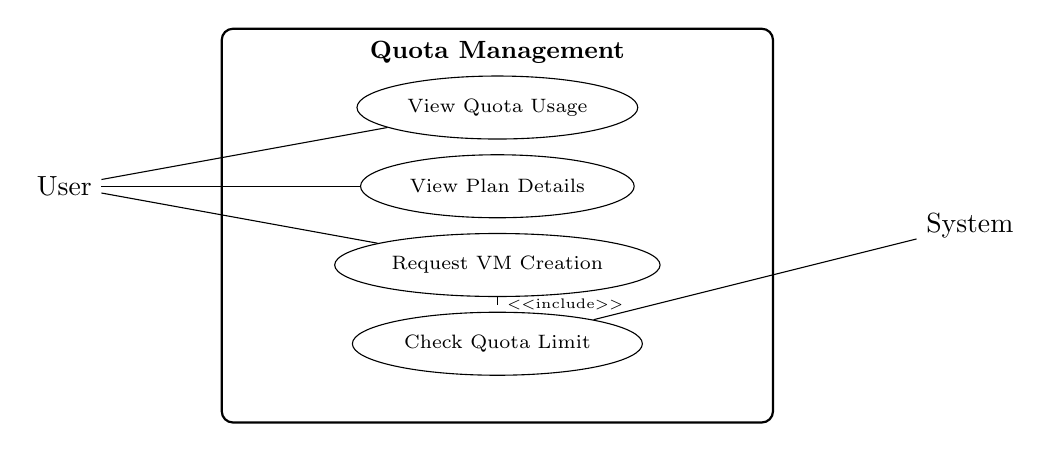
\begin{tikzpicture}[
  usecase/.style={draw, ellipse, minimum width=3cm, minimum height=0.8cm, align=center, font=\scriptsize}
]
  \draw[thick, rounded corners] (0, -4.5) rectangle (7, 0.5);
  \node[font=\small\bfseries] at (3.5, 0.2) {Quota Management};
  
  \node (user) at (-2, -1.5) {User};
  \node (system) at (9.5, -2) {System};
  
  \node[usecase] (uc1) at (3.5, -0.5) {View Quota Usage};
  \node[usecase] (uc2) at (3.5, -1.5) {View Plan Details};
  \node[usecase] (uc3) at (3.5, -2.5) {Request VM Creation};
  \node[usecase] (uc4) at (3.5, -3.5) {Check Quota Limit};
  
  \draw (user) -- (uc1);
  \draw (user) -- (uc2);
  \draw (user) -- (uc3);
  \draw[dashed] (uc3) -- node[right, font=\tiny] {<<include>>} (uc4);
  \draw (system) -- (uc4);
\end{tikzpicture}
\caption{Use case diagram — Quota management}
\label{fig:uc-quota}
\end{figure}

\subsection{Sequence Diagram — Quota Check on VM Creation}

\begin{figure}[H]
\centering
\begin{tikzpicture}[font=\small]
  \node (user) at (0, 0) {\textbf{User}};
  \node (vmsvc) at (4, 0) {\textbf{VM Service}};
  \node (quota) at (8, 0) {\textbf{Quota Service}};
  \node (db) at (12, 0) {\textbf{Database}};
  
  \draw[dashed] (user) -- (0, -8);
  \draw[dashed] (vmsvc) -- (4, -8);
  \draw[dashed] (quota) -- (8, -8);
  \draw[dashed] (db) -- (12, -8);
  
  \draw[->, thick] (0, -1) -- node[above, font=\tiny] {Create VM request} (4, -1);
  \draw[->, thick] (4, -2) -- node[above, font=\tiny] {Check user quota} (8, -2);
  \draw[->, thick] (8, -3) -- node[above, font=\tiny] {Get user plan + VM count} (12, -3);
  \draw[<-, thick] (8, -3.5) -- node[above, font=\tiny] {Plan: Pro, VMs: 3/5} (12, -3.5);
  \draw[<-, thick] (4, -4.5) -- node[above, font=\tiny] {Quota OK (3 < 5)} (8, -4.5);
  \draw[->, thick] (4, -5.5) -- node[right, font=\tiny] {Proceed with creation};
  
  % Alternative (quota exceeded)
  \draw[thick, red, dashed] (1, -6) rectangle (11, -7.5);
  \node[red, font=\tiny] at (6, -6.3) {alt: Quota Exceeded};
  \draw[->, thick, red] (8, -7) -- node[above, font=\tiny, red] {403 Quota Exceeded} (4, -7);
\end{tikzpicture}
\caption{Sequence diagram — Quota check on VM creation}
\label{fig:seq-quota}
\end{figure}

\subsection{Class Diagram — Quota \& Plan}

\begin{figure}[H]
\centering
\begin{tikzpicture}[font=\small,
  class/.style={draw, rectangle, minimum width=3.5cm, align=left}
]
  \node[class, fill=yellow!15] (plan) at (0, 0) {
    \textbf{Plan}\\
    \hline
    - id: UUID\\
    - name: String\\
    - maxVMs: Integer\\
    - maxCPU: Integer\\
    - maxRAM: Integer\\
    - maxDisk: Integer\\
    - price: Decimal\\
    \hline
    + getPlans()
  };
  
  \node[class, fill=blue!15] (quota) at (6, 0) {
    \textbf{UserQuota}\\
    \hline
    - id: UUID\\
    - userId: UUID\\
    - planId: UUID\\
    - usedVMs: Integer\\
    - usedCPU: Integer\\
    - usedRAM: Integer\\
    - usedDisk: Integer\\
    \hline
    + checkLimit()\\
    + updateUsage()
  };
  
  \draw[->, thick] (quota) -- node[above, font=\tiny] {belongs to} (plan);
\end{tikzpicture}
\caption{Class diagram — Plan and quota}
\label{fig:class-quota}
\end{figure}

\subsection{Implementation Screenshots}

\begin{figure}[H]
\centering
\fbox{\parbox{0.9\textwidth}{\centering\vspace{3cm}\textit{Insert VM detail page screenshot}\vspace{3cm}}}
\caption{VM detail page with status, IP, and resources}
\label{fig:vm-detail}
\end{figure}

\begin{figure}[H]
\centering
\fbox{\parbox{0.9\textwidth}{\centering\vspace{3cm}\textit{Insert quota usage display screenshot}\vspace{3cm}}}
\caption{Dashboard — Quota usage display}
\label{fig:quota-display}
\end{figure}
\subsection{Sequence Diagram --- Web Terminal Connection}

\begin{figure}[H]
\centering
\begin{tikzpicture}[font=\small]
  \node (user) at (0, 0) {\textbf{User}};
  \node (front) at (3, 0) {\textbf{Frontend}};
  \node (gate) at (6, 0) {\textbf{Gateway}};
  \node (proxy) at (9, 0) {\textbf{SSH Proxy}};
  \node (vm) at (12, 0) {\textbf{VM (SSH)}};
  
  \draw[dashed] (user) -- (0, -9);
  \draw[dashed] (front) -- (3, -9);
  \draw[dashed] (gate) -- (6, -9);
  \draw[dashed] (proxy) -- (9, -9);
  \draw[dashed] (vm) -- (12, -9);
  
  \draw[->, thick] (0, -0.8) -- node[above, font=\tiny] {Click ``Terminal''} (3, -0.8);
  \draw[->, thick] (3, -1.5) -- node[above, font=\tiny] {WebSocket connect} (6, -1.5);
  \draw[->, thick] (6, -2.2) -- node[above, font=\tiny] {Get user SSH key} (6, -2.2);
  \draw[->, thick] (6, -2.7) -- node[right, font=\tiny] {Verify JWT};
  \draw[->, thick] (6, -3.5) -- node[above, font=\tiny] {Open SSH tunnel} (9, -3.5);
  \draw[->, thick] (9, -4.2) -- node[above, font=\tiny] {SSH connect (key auth)} (12, -4.2);
  \draw[<-, thick] (9, -4.9) -- node[above, font=\tiny] {Shell session open} (12, -4.9);
  \draw[<-, thick] (6, -5.6) -- node[above, font=\tiny] {Tunnel ready} (9, -5.6);
  \draw[<-, thick] (3, -6.3) -- node[above, font=\tiny] {WS connected} (6, -6.3);
  \draw[->, thick] (3, -7) -- node[below, font=\tiny] {xterm.js renders terminal} (3, -7);
  \draw[<->, thick] (0, -7.5) -- node[above, font=\tiny] {Type commands / see output} (3, -7.5);
  \draw[<->, thick, blue, dashed] (3, -8.2) -- node[above, font=\tiny, blue] {Bidirectional data stream} (12, -8.2);
\end{tikzpicture}
\caption{Sequence diagram --- Web terminal connection (Phase~1)}
\label{fig:seq-terminal}
\end{figure}

\begin{figure}[H]
\centering
\fbox{\parbox{0.9\textwidth}{\centering\vspace{3cm}\textit{Insert web terminal (CLI) screenshot --- user accessing VM from browser}\vspace{3cm}}}
\caption{Web terminal --- CLI access to VM via xterm.js (Phase~1)}
\label{fig:web-terminal}
\end{figure}
\subsection{Sprint 5 Review}

At the end of Sprint 5:
\begin{itemize}
  \item VM detail page showing IP, status, OS, CPU, RAM, uptime.
  \item \textbf{Web terminal (Phase~1)} --- users can access VMs via a CLI terminal in the browser using xterm.js and WebSocket SSH proxy.
  \item VM action buttons (start, stop, reboot, delete) with confirmation dialogs.
  \item Quota system tracking and enforcing resource limits.
  \item Admin VM management page with filtering.
  \item Server monitoring and backup procedures in place.
\end{itemize}


% ============================================================
% SPRINT 6
% ============================================================
\section{Sprint 6: Payment Service}

\sprintcard{6}{Payment Service}{Implement payment processing with plan management, upgrade flows, and billing history.}

\subsection{Sprint Backlog}

\begin{longtable}{|c|p{5cm}|c|c|c|}
\hline
\rowcolor{blue!15}
\textbf{Task ID} & \textbf{Task} & \textbf{Assignee} & \textbf{Est.} & \textbf{Status} \\
\hline
\endhead
T-6.1 & Plans CRUD (backend) & DSI & 4h & Done \\
\hline
T-6.2 & Payment processing (Stripe/mock) & DSI & 5h & Done \\
\hline
T-6.3 & Billing page (frontend) & DSI & 4h & Done \\
\hline
T-6.4 & Checkout flow (frontend) & DSI & 5h & Done \\
\hline
T-6.5 & Payment history page & DSI & 3h & Done \\
\hline
T-6.6 & Admin plan management page & DSI & 3h & Done \\
\hline
T-6.7 & SSL/TLS configuration & RSI & 4h & Done \\
\hline
T-6.8 & Log management & RSI & 4h & Done \\
\hline
T-6.9 & OpenNebula optimization & RSI & 4h & Done \\
\hline
\caption{Sprint 6 backlog}
\label{tab:sprint6-backlog}
\end{longtable}

\subsection{Use Case Diagram — Payment}

\begin{figure}[H]
\centering
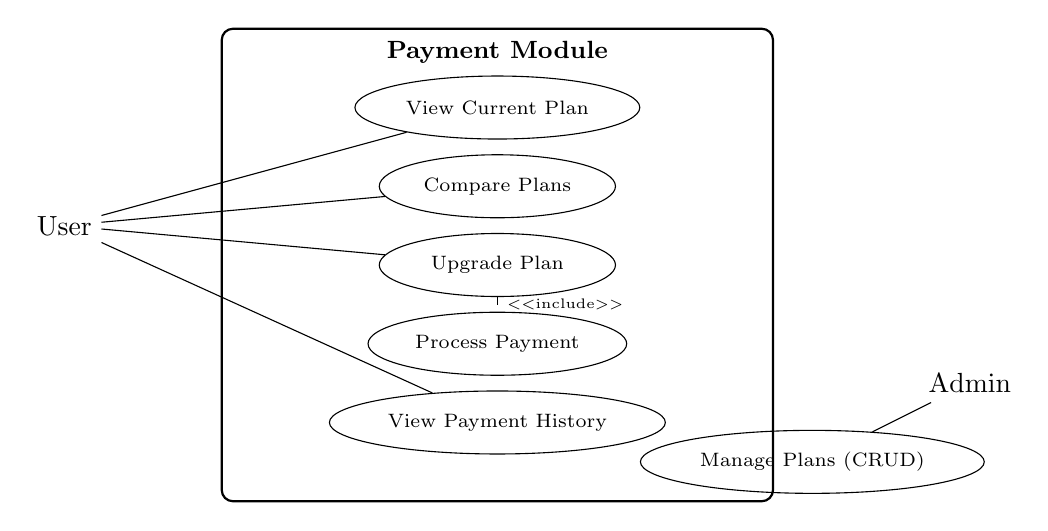
\begin{tikzpicture}[
  usecase/.style={draw, ellipse, minimum width=3cm, minimum height=0.8cm, align=center, font=\scriptsize}
]
  \draw[thick, rounded corners] (0, -5.5) rectangle (7, 0.5);
  \node[font=\small\bfseries] at (3.5, 0.2) {Payment Module};
  
  \node (user) at (-2, -2) {User};
  \node (admin) at (9.5, -4) {Admin};
  
  \node[usecase] (uc1) at (3.5, -0.5) {View Current Plan};
  \node[usecase] (uc2) at (3.5, -1.5) {Compare Plans};
  \node[usecase] (uc3) at (3.5, -2.5) {Upgrade Plan};
  \node[usecase] (uc4) at (3.5, -3.5) {Process Payment};
  \node[usecase] (uc5) at (3.5, -4.5) {View Payment History};
  
  \draw (user) -- (uc1);
  \draw (user) -- (uc2);
  \draw (user) -- (uc3);
  \draw (user) -- (uc5);
  \draw[dashed] (uc3) -- node[right, font=\tiny] {<<include>>} (uc4);
  
  \node[usecase] (uc6) at (7.5, -5) {Manage Plans (CRUD)};
  \draw (admin) -- (uc6);
\end{tikzpicture}
\caption{Use case diagram — Payment module}
\label{fig:uc-payment}
\end{figure}

\subsection{Sequence Diagram — Plan Upgrade}

\begin{figure}[H]
\centering
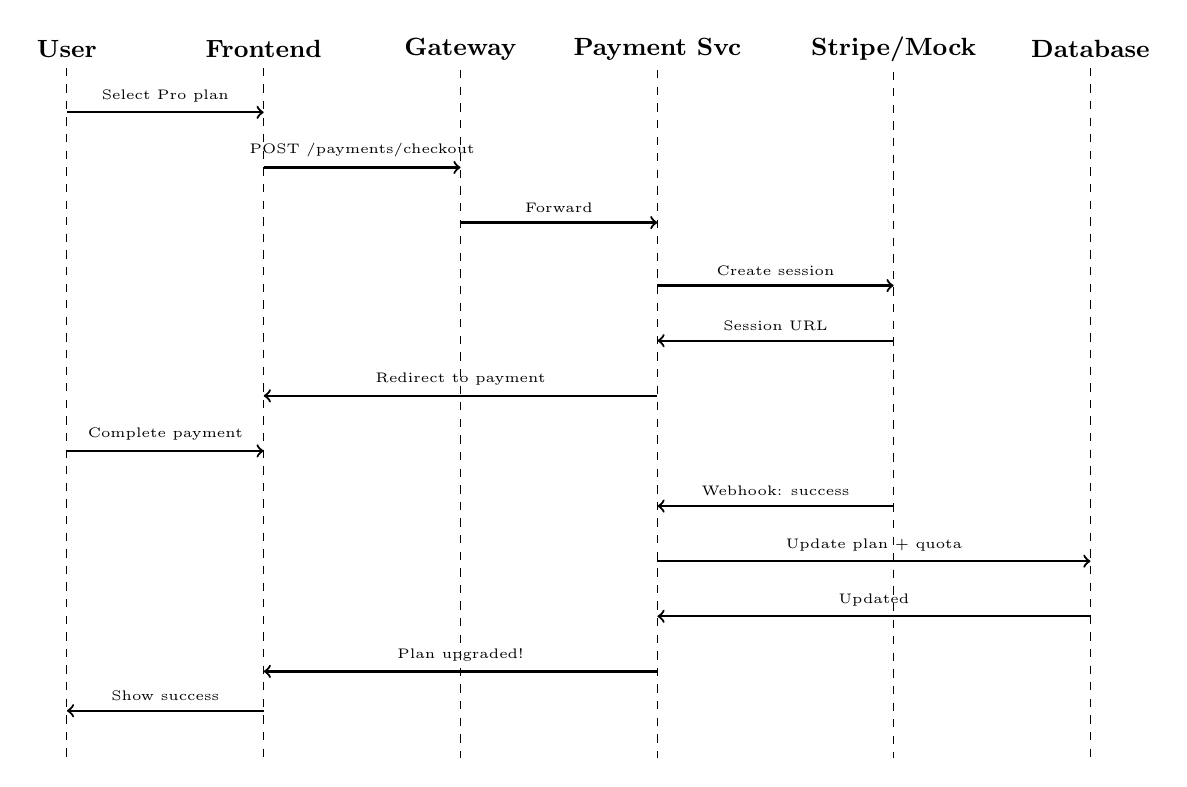
\begin{tikzpicture}[font=\small]
  \node (user) at (0, 0) {\textbf{User}};
  \node (front) at (2.5, 0) {\textbf{Frontend}};
  \node (gate) at (5, 0) {\textbf{Gateway}};
  \node (pay) at (7.5, 0) {\textbf{Payment Svc}};
  \node (stripe) at (10.5, 0) {\textbf{Stripe/Mock}};
  \node (db) at (13, 0) {\textbf{Database}};
  
  \draw[dashed] (user) -- (0, -9);
  \draw[dashed] (front) -- (2.5, -9);
  \draw[dashed] (gate) -- (5, -9);
  \draw[dashed] (pay) -- (7.5, -9);
  \draw[dashed] (stripe) -- (10.5, -9);
  \draw[dashed] (db) -- (13, -9);
  
  \draw[->, thick] (0, -0.8) -- node[above, font=\tiny] {Select Pro plan} (2.5, -0.8);
  \draw[->, thick] (2.5, -1.5) -- node[above, font=\tiny] {POST /payments/checkout} (5, -1.5);
  \draw[->, thick] (5, -2.2) -- node[above, font=\tiny] {Forward} (7.5, -2.2);
  \draw[->, thick] (7.5, -3) -- node[above, font=\tiny] {Create session} (10.5, -3);
  \draw[<-, thick] (7.5, -3.7) -- node[above, font=\tiny] {Session URL} (10.5, -3.7);
  \draw[<-, thick] (2.5, -4.4) -- node[above, font=\tiny] {Redirect to payment} (7.5, -4.4);
  \draw[->, thick] (0, -5.1) -- node[above, font=\tiny] {Complete payment} (2.5, -5.1);
  \draw[->, thick] (10.5, -5.8) -- node[above, font=\tiny] {Webhook: success} (7.5, -5.8);
  \draw[->, thick] (7.5, -6.5) -- node[above, font=\tiny] {Update plan + quota} (13, -6.5);
  \draw[<-, thick] (7.5, -7.2) -- node[above, font=\tiny] {Updated} (13, -7.2);
  \draw[<-, thick] (2.5, -7.9) -- node[above, font=\tiny] {Plan upgraded!} (7.5, -7.9);
  \draw[<-, thick] (0, -8.4) -- node[above, font=\tiny] {Show success} (2.5, -8.4);
\end{tikzpicture}
\caption{Sequence diagram — Plan upgrade with payment}
\label{fig:seq-payment}
\end{figure}

\subsection{Class Diagram — Payment Module}

\begin{figure}[H]
\centering
\begin{tikzpicture}[font=\small,
  class/.style={draw, rectangle, minimum width=3.5cm, align=left}
]
  \node[class, fill=yellow!15] (payment) at (0, 0) {
    \textbf{Payment}\\
    \hline
    - id: UUID\\
    - userId: UUID\\
    - planId: UUID\\
    - amount: Decimal\\
    - currency: String\\
    - status: PaymentStatus\\
    - stripeSessionId: String\\
    - createdAt: DateTime\\
    \hline
    + createCheckout()\\
    + processWebhook()
  };
  
  \node[class, fill=green!15] (pstatus) at (6, 0) {
    \textbf{<<enum>> PaymentStatus}\\
    \hline
    PENDING\\
    COMPLETED\\
    FAILED\\
    REFUNDED
  };
  
  \node[class, fill=blue!15] (invoice) at (0, -4.5) {
    \textbf{Invoice}\\
    \hline
    - id: UUID\\
    - paymentId: UUID\\
    - invoiceNumber: String\\
    - pdfUrl: String\\
    - createdAt: DateTime\\
    \hline
    + generate()
  };
  
  \draw[->, thick] (payment) -- (pstatus);
  \draw[->, thick] (payment) -- node[left, font=\tiny] {generates} (invoice);
\end{tikzpicture}
\caption{Class diagram — Payment module}
\label{fig:class-payment}
\end{figure}

\subsection{Implementation Screenshots}

\begin{figure}[H]
\centering
\fbox{\parbox{0.9\textwidth}{\centering\vspace{3cm}\textit{Insert billing page screenshot}\vspace{3cm}}}
\caption{Billing page — Current plan and usage}
\label{fig:billing-page}
\end{figure}

\begin{figure}[H]
\centering
\fbox{\parbox{0.9\textwidth}{\centering\vspace{3cm}\textit{Insert checkout flow screenshot}\vspace{3cm}}}
\caption{Checkout flow — Plan upgrade}
\label{fig:checkout}
\end{figure}

\begin{figure}[H]
\centering
\fbox{\parbox{0.9\textwidth}{\centering\vspace{3cm}\textit{Insert payment history screenshot}\vspace{3cm}}}
\caption{Payment history page}
\label{fig:payment-history}
\end{figure}

\subsection{Sprint 6 Review}

At the end of Sprint 6:
\begin{itemize}
  \item Payment service with plan CRUD and checkout.
  \item Stripe/mock payment processing with webhooks.
  \item Billing page displaying current plan and usage.
  \item Checkout flow for plan upgrades.
  \item Payment history with transaction records.
  \item Admin plan management page.
  \item SSL/TLS configured on the server.
\end{itemize}

% ============================================================
\section{Conclusion}

This chapter delivered the business layer of the platform. Sprint 5 enhanced the VM experience with detailed monitoring, \textbf{web-based CLI terminal access (Phase~1)}, and enforced resource limits through the quota system. Sprint 6 completed the monetization aspect with a full payment service supporting plan upgrades and billing history.

In the next chapter, we will finalize the platform with notifications, comprehensive testing, deployment, and project documentation.

% ============================================================
\chapter{Sprint 5 \& Sprint 6: Quotas and Payment Service}

\section{Introduction}

This chapter covers the business logic layer of the platform. Sprint 5 implements the VM dashboard with detailed information and the quota system that enforces resource limits per user. Sprint 6 delivers the payment service with plan management and upgrade flows.

% ============================================================
% SPRINT 5
% ============================================================
\section{Sprint 5: VM Dashboard \& Quota System}

\sprintcard{5}{VM Dashboard \& Quota System}{Deliver a comprehensive VM dashboard with status monitoring, and implement quota enforcement to limit resource usage per plan.}

\subsection{Sprint Backlog}

\begin{longtable}{|c|p{5cm}|c|c|c|}
\hline
\rowcolor{blue!15}
\textbf{Task ID} & \textbf{Task} & \textbf{Assignee} & \textbf{Est.} & \textbf{Status} \\
\hline
\endhead
T-5.1 & VM detail page (frontend) & DSI & 5h & Done \\
\hline
T-5.10 & Web terminal (xterm.js + WebSocket SSH) & DSI & 6h & Done \\
\hline
T-5.2 & VM action buttons + confirmation & DSI & 4h & Done \\
\hline
T-5.3 & Quota tracking implementation & DSI & 4h & Done \\
\hline
T-5.4 & Quota enforcement on VM creation & DSI & 3h & Done \\
\hline
T-5.5 & Admin VM management page & DSI & 5h & Done \\
\hline
T-5.6 & Quota display on dashboard & DSI & 3h & Done \\
\hline
T-5.7 & Server monitoring setup & RSI & 6h & Done \\
\hline
T-5.8 & Backup procedures & RSI & 4h & Done \\
\hline
T-5.9 & Network security audit & RSI & 4h & Done \\
\hline
\caption{Sprint 5 backlog}
\label{tab:sprint5-backlog}
\end{longtable}

\subsection{Use Case Diagram — Quota Management}

\begin{figure}[H]
\centering
\begin{tikzpicture}[
  usecase/.style={draw, ellipse, minimum width=3cm, minimum height=0.8cm, align=center, font=\scriptsize}
]
  \draw[thick, rounded corners] (0, -4.5) rectangle (7, 0.5);
  \node[font=\small\bfseries] at (3.5, 0.2) {Quota Management};
  
  \node (user) at (-2, -1.5) {User};
  \node (system) at (9.5, -2) {System};
  
  \node[usecase] (uc1) at (3.5, -0.5) {View Quota Usage};
  \node[usecase] (uc2) at (3.5, -1.5) {View Plan Details};
  \node[usecase] (uc3) at (3.5, -2.5) {Request VM Creation};
  \node[usecase] (uc4) at (3.5, -3.5) {Check Quota Limit};
  
  \draw (user) -- (uc1);
  \draw (user) -- (uc2);
  \draw (user) -- (uc3);
  \draw[dashed] (uc3) -- node[right, font=\tiny] {<<include>>} (uc4);
  \draw (system) -- (uc4);
\end{tikzpicture}
\caption{Use case diagram — Quota management}
\label{fig:uc-quota}
\end{figure}

\subsection{Sequence Diagram — Quota Check on VM Creation}

\begin{figure}[H]
\centering
\begin{tikzpicture}[font=\small]
  \node (user) at (0, 0) {\textbf{User}};
  \node (vmsvc) at (4, 0) {\textbf{VM Service}};
  \node (quota) at (8, 0) {\textbf{Quota Service}};
  \node (db) at (12, 0) {\textbf{Database}};
  
  \draw[dashed] (user) -- (0, -8);
  \draw[dashed] (vmsvc) -- (4, -8);
  \draw[dashed] (quota) -- (8, -8);
  \draw[dashed] (db) -- (12, -8);
  
  \draw[->, thick] (0, -1) -- node[above, font=\tiny] {Create VM request} (4, -1);
  \draw[->, thick] (4, -2) -- node[above, font=\tiny] {Check user quota} (8, -2);
  \draw[->, thick] (8, -3) -- node[above, font=\tiny] {Get user plan + VM count} (12, -3);
  \draw[<-, thick] (8, -3.5) -- node[above, font=\tiny] {Plan: Pro, VMs: 3/5} (12, -3.5);
  \draw[<-, thick] (4, -4.5) -- node[above, font=\tiny] {Quota OK (3 < 5)} (8, -4.5);
  \draw[->, thick] (4, -5.5) -- node[right, font=\tiny] {Proceed with creation};
  
  % Alternative (quota exceeded)
  \draw[thick, red, dashed] (1, -6) rectangle (11, -7.5);
  \node[red, font=\tiny] at (6, -6.3) {alt: Quota Exceeded};
  \draw[->, thick, red] (8, -7) -- node[above, font=\tiny, red] {403 Quota Exceeded} (4, -7);
\end{tikzpicture}
\caption{Sequence diagram — Quota check on VM creation}
\label{fig:seq-quota}
\end{figure}

\subsection{Class Diagram — Quota \& Plan}

\begin{figure}[H]
\centering
\begin{tikzpicture}[font=\small,
  class/.style={draw, rectangle, minimum width=3.5cm, align=left}
]
  \node[class, fill=yellow!15] (plan) at (0, 0) {
    \textbf{Plan}\\
    \hline
    - id: UUID\\
    - name: String\\
    - maxVMs: Integer\\
    - maxCPU: Integer\\
    - maxRAM: Integer\\
    - maxDisk: Integer\\
    - price: Decimal\\
    \hline
    + getPlans()
  };
  
  \node[class, fill=blue!15] (quota) at (6, 0) {
    \textbf{UserQuota}\\
    \hline
    - id: UUID\\
    - userId: UUID\\
    - planId: UUID\\
    - usedVMs: Integer\\
    - usedCPU: Integer\\
    - usedRAM: Integer\\
    - usedDisk: Integer\\
    \hline
    + checkLimit()\\
    + updateUsage()
  };
  
  \draw[->, thick] (quota) -- node[above, font=\tiny] {belongs to} (plan);
\end{tikzpicture}
\caption{Class diagram — Plan and quota}
\label{fig:class-quota}
\end{figure}

\subsection{Implementation Screenshots}

\begin{figure}[H]
\centering
\fbox{\parbox{0.9\textwidth}{\centering\vspace{3cm}\textit{Insert VM detail page screenshot}\vspace{3cm}}}
\caption{VM detail page with status, IP, and resources}
\label{fig:vm-detail}
\end{figure}

\begin{figure}[H]
\centering
\fbox{\parbox{0.9\textwidth}{\centering\vspace{3cm}\textit{Insert quota usage display screenshot}\vspace{3cm}}}
\caption{Dashboard — Quota usage display}
\label{fig:quota-display}
\end{figure}
\subsection{Sequence Diagram --- Web Terminal Connection}

\begin{figure}[H]
\centering
\begin{tikzpicture}[font=\small]
  \node (user) at (0, 0) {\textbf{User}};
  \node (front) at (3, 0) {\textbf{Frontend}};
  \node (gate) at (6, 0) {\textbf{Gateway}};
  \node (proxy) at (9, 0) {\textbf{SSH Proxy}};
  \node (vm) at (12, 0) {\textbf{VM (SSH)}};
  
  \draw[dashed] (user) -- (0, -9);
  \draw[dashed] (front) -- (3, -9);
  \draw[dashed] (gate) -- (6, -9);
  \draw[dashed] (proxy) -- (9, -9);
  \draw[dashed] (vm) -- (12, -9);
  
  \draw[->, thick] (0, -0.8) -- node[above, font=\tiny] {Click ``Terminal''} (3, -0.8);
  \draw[->, thick] (3, -1.5) -- node[above, font=\tiny] {WebSocket connect} (6, -1.5);
  \draw[->, thick] (6, -2.2) -- node[above, font=\tiny] {Get user SSH key} (6, -2.2);
  \draw[->, thick] (6, -2.7) -- node[right, font=\tiny] {Verify JWT};
  \draw[->, thick] (6, -3.5) -- node[above, font=\tiny] {Open SSH tunnel} (9, -3.5);
  \draw[->, thick] (9, -4.2) -- node[above, font=\tiny] {SSH connect (key auth)} (12, -4.2);
  \draw[<-, thick] (9, -4.9) -- node[above, font=\tiny] {Shell session open} (12, -4.9);
  \draw[<-, thick] (6, -5.6) -- node[above, font=\tiny] {Tunnel ready} (9, -5.6);
  \draw[<-, thick] (3, -6.3) -- node[above, font=\tiny] {WS connected} (6, -6.3);
  \draw[->, thick] (3, -7) -- node[below, font=\tiny] {xterm.js renders terminal} (3, -7);
  \draw[<->, thick] (0, -7.5) -- node[above, font=\tiny] {Type commands / see output} (3, -7.5);
  \draw[<->, thick, blue, dashed] (3, -8.2) -- node[above, font=\tiny, blue] {Bidirectional data stream} (12, -8.2);
\end{tikzpicture}
\caption{Sequence diagram --- Web terminal connection (Phase~1)}
\label{fig:seq-terminal}
\end{figure}

\begin{figure}[H]
\centering
\fbox{\parbox{0.9\textwidth}{\centering\vspace{3cm}\textit{Insert web terminal (CLI) screenshot --- user accessing VM from browser}\vspace{3cm}}}
\caption{Web terminal --- CLI access to VM via xterm.js (Phase~1)}
\label{fig:web-terminal}
\end{figure}
\subsection{Sprint 5 Review}

At the end of Sprint 5:
\begin{itemize}
  \item VM detail page showing IP, status, OS, CPU, RAM, uptime.
  \item \textbf{Web terminal (Phase~1)} --- users can access VMs via a CLI terminal in the browser using xterm.js and WebSocket SSH proxy.
  \item VM action buttons (start, stop, reboot, delete) with confirmation dialogs.
  \item Quota system tracking and enforcing resource limits.
  \item Admin VM management page with filtering.
  \item Server monitoring and backup procedures in place.
\end{itemize}


% ============================================================
% SPRINT 6
% ============================================================
\section{Sprint 6: Payment Service}

\sprintcard{6}{Payment Service}{Implement payment processing with plan management, upgrade flows, and billing history.}

\subsection{Sprint Backlog}

\begin{longtable}{|c|p{5cm}|c|c|c|}
\hline
\rowcolor{blue!15}
\textbf{Task ID} & \textbf{Task} & \textbf{Assignee} & \textbf{Est.} & \textbf{Status} \\
\hline
\endhead
T-6.1 & Plans CRUD (backend) & DSI & 4h & Done \\
\hline
T-6.2 & Payment processing (Stripe/mock) & DSI & 5h & Done \\
\hline
T-6.3 & Billing page (frontend) & DSI & 4h & Done \\
\hline
T-6.4 & Checkout flow (frontend) & DSI & 5h & Done \\
\hline
T-6.5 & Payment history page & DSI & 3h & Done \\
\hline
T-6.6 & Admin plan management page & DSI & 3h & Done \\
\hline
T-6.7 & SSL/TLS configuration & RSI & 4h & Done \\
\hline
T-6.8 & Log management & RSI & 4h & Done \\
\hline
T-6.9 & OpenNebula optimization & RSI & 4h & Done \\
\hline
\caption{Sprint 6 backlog}
\label{tab:sprint6-backlog}
\end{longtable}

\subsection{Use Case Diagram — Payment}

\begin{figure}[H]
\centering
\begin{tikzpicture}[
  usecase/.style={draw, ellipse, minimum width=3cm, minimum height=0.8cm, align=center, font=\scriptsize}
]
  \draw[thick, rounded corners] (0, -5.5) rectangle (7, 0.5);
  \node[font=\small\bfseries] at (3.5, 0.2) {Payment Module};
  
  \node (user) at (-2, -2) {User};
  \node (admin) at (9.5, -4) {Admin};
  
  \node[usecase] (uc1) at (3.5, -0.5) {View Current Plan};
  \node[usecase] (uc2) at (3.5, -1.5) {Compare Plans};
  \node[usecase] (uc3) at (3.5, -2.5) {Upgrade Plan};
  \node[usecase] (uc4) at (3.5, -3.5) {Process Payment};
  \node[usecase] (uc5) at (3.5, -4.5) {View Payment History};
  
  \draw (user) -- (uc1);
  \draw (user) -- (uc2);
  \draw (user) -- (uc3);
  \draw (user) -- (uc5);
  \draw[dashed] (uc3) -- node[right, font=\tiny] {<<include>>} (uc4);
  
  \node[usecase] (uc6) at (7.5, -5) {Manage Plans (CRUD)};
  \draw (admin) -- (uc6);
\end{tikzpicture}
\caption{Use case diagram — Payment module}
\label{fig:uc-payment}
\end{figure}

\subsection{Sequence Diagram — Plan Upgrade}

\begin{figure}[H]
\centering
\begin{tikzpicture}[font=\small]
  \node (user) at (0, 0) {\textbf{User}};
  \node (front) at (2.5, 0) {\textbf{Frontend}};
  \node (gate) at (5, 0) {\textbf{Gateway}};
  \node (pay) at (7.5, 0) {\textbf{Payment Svc}};
  \node (stripe) at (10.5, 0) {\textbf{Stripe/Mock}};
  \node (db) at (13, 0) {\textbf{Database}};
  
  \draw[dashed] (user) -- (0, -9);
  \draw[dashed] (front) -- (2.5, -9);
  \draw[dashed] (gate) -- (5, -9);
  \draw[dashed] (pay) -- (7.5, -9);
  \draw[dashed] (stripe) -- (10.5, -9);
  \draw[dashed] (db) -- (13, -9);
  
  \draw[->, thick] (0, -0.8) -- node[above, font=\tiny] {Select Pro plan} (2.5, -0.8);
  \draw[->, thick] (2.5, -1.5) -- node[above, font=\tiny] {POST /payments/checkout} (5, -1.5);
  \draw[->, thick] (5, -2.2) -- node[above, font=\tiny] {Forward} (7.5, -2.2);
  \draw[->, thick] (7.5, -3) -- node[above, font=\tiny] {Create session} (10.5, -3);
  \draw[<-, thick] (7.5, -3.7) -- node[above, font=\tiny] {Session URL} (10.5, -3.7);
  \draw[<-, thick] (2.5, -4.4) -- node[above, font=\tiny] {Redirect to payment} (7.5, -4.4);
  \draw[->, thick] (0, -5.1) -- node[above, font=\tiny] {Complete payment} (2.5, -5.1);
  \draw[->, thick] (10.5, -5.8) -- node[above, font=\tiny] {Webhook: success} (7.5, -5.8);
  \draw[->, thick] (7.5, -6.5) -- node[above, font=\tiny] {Update plan + quota} (13, -6.5);
  \draw[<-, thick] (7.5, -7.2) -- node[above, font=\tiny] {Updated} (13, -7.2);
  \draw[<-, thick] (2.5, -7.9) -- node[above, font=\tiny] {Plan upgraded!} (7.5, -7.9);
  \draw[<-, thick] (0, -8.4) -- node[above, font=\tiny] {Show success} (2.5, -8.4);
\end{tikzpicture}
\caption{Sequence diagram — Plan upgrade with payment}
\label{fig:seq-payment}
\end{figure}

\subsection{Class Diagram — Payment Module}

\begin{figure}[H]
\centering
\begin{tikzpicture}[font=\small,
  class/.style={draw, rectangle, minimum width=3.5cm, align=left}
]
  \node[class, fill=yellow!15] (payment) at (0, 0) {
    \textbf{Payment}\\
    \hline
    - id: UUID\\
    - userId: UUID\\
    - planId: UUID\\
    - amount: Decimal\\
    - currency: String\\
    - status: PaymentStatus\\
    - stripeSessionId: String\\
    - createdAt: DateTime\\
    \hline
    + createCheckout()\\
    + processWebhook()
  };
  
  \node[class, fill=green!15] (pstatus) at (6, 0) {
    \textbf{<<enum>> PaymentStatus}\\
    \hline
    PENDING\\
    COMPLETED\\
    FAILED\\
    REFUNDED
  };
  
  \node[class, fill=blue!15] (invoice) at (0, -4.5) {
    \textbf{Invoice}\\
    \hline
    - id: UUID\\
    - paymentId: UUID\\
    - invoiceNumber: String\\
    - pdfUrl: String\\
    - createdAt: DateTime\\
    \hline
    + generate()
  };
  
  \draw[->, thick] (payment) -- (pstatus);
  \draw[->, thick] (payment) -- node[left, font=\tiny] {generates} (invoice);
\end{tikzpicture}
\caption{Class diagram — Payment module}
\label{fig:class-payment}
\end{figure}

\subsection{Implementation Screenshots}

\begin{figure}[H]
\centering
\fbox{\parbox{0.9\textwidth}{\centering\vspace{3cm}\textit{Insert billing page screenshot}\vspace{3cm}}}
\caption{Billing page — Current plan and usage}
\label{fig:billing-page}
\end{figure}

\begin{figure}[H]
\centering
\fbox{\parbox{0.9\textwidth}{\centering\vspace{3cm}\textit{Insert checkout flow screenshot}\vspace{3cm}}}
\caption{Checkout flow — Plan upgrade}
\label{fig:checkout}
\end{figure}

\begin{figure}[H]
\centering
\fbox{\parbox{0.9\textwidth}{\centering\vspace{3cm}\textit{Insert payment history screenshot}\vspace{3cm}}}
\caption{Payment history page}
\label{fig:payment-history}
\end{figure}

\subsection{Sprint 6 Review}

At the end of Sprint 6:
\begin{itemize}
  \item Payment service with plan CRUD and checkout.
  \item Stripe/mock payment processing with webhooks.
  \item Billing page displaying current plan and usage.
  \item Checkout flow for plan upgrades.
  \item Payment history with transaction records.
  \item Admin plan management page.
  \item SSL/TLS configured on the server.
\end{itemize}

% ============================================================
\section{Conclusion}

This chapter delivered the business layer of the platform. Sprint 5 enhanced the VM experience with detailed monitoring, \textbf{web-based CLI terminal access (Phase~1)}, and enforced resource limits through the quota system. Sprint 6 completed the monetization aspect with a full payment service supporting plan upgrades and billing history.

In the next chapter, we will finalize the platform with notifications, comprehensive testing, deployment, and project documentation.


% ============================================================
% CHAPTER 5: Sprint 7 & 8 (Testing + Deployment)
% ============================================================
% % ============================================================
% CHAPTER 5: Sprint 7 & Sprint 8 — Polish, Testing & Deployment
% ============================================================
% ADD THIS TO main.tex AFTER COMPLETING SPRINT 7 & 8
% Uncomment: % ============================================================
% CHAPTER 5: Sprint 7 & Sprint 8 — Polish, Testing & Deployment
% ============================================================
% ADD THIS TO main.tex AFTER COMPLETING SPRINT 7 & 8
% Uncomment: % ============================================================
% CHAPTER 5: Sprint 7 & Sprint 8 — Polish, Testing & Deployment
% ============================================================
% ADD THIS TO main.tex AFTER COMPLETING SPRINT 7 & 8
% Uncomment: \input{chapters/chapter5}
% ============================================================
\chapter{Sprint 7 \& Sprint 8: Testing, Deployment and Finalization}

\section{Introduction}

This final chapter covers the last two sprints of the project. Sprint 7 focuses on notifications, UI polish, and comprehensive integration testing. Sprint 8 handles production deployment, final documentation, and presentation preparation.

% ============================================================
% SPRINT 7
% ============================================================
\section{Sprint 7: Notifications \& Integration Testing}

\sprintcard{7}{Notifications \& Integration Testing}{Implement notification system, polish the UI, and conduct thorough integration testing across all features.}

\subsection{Sprint Backlog}

\begin{longtable}{|c|p{5cm}|c|c|c|}
\hline
\rowcolor{blue!15}
\textbf{Task ID} & \textbf{Task} & \textbf{Assignee} & \textbf{Est.} & \textbf{Status} \\
\hline
\endhead
T-7.1 & Notification service (backend) & DSI & 4h & Done \\
\hline
T-7.2 & In-app notification UI & DSI & 3h & Done \\
\hline
T-7.3 & Error handling improvements & DSI & 4h & Done \\
\hline
T-7.4 & UI polish (loading, animations) & DSI & 5h & Done \\
\hline
T-7.5 & Integration testing & DSI & 6h & Done \\
\hline
T-7.6 & Bug fixes & DSI & 4h & Done \\
\hline
T-7.7 & Server end-to-end testing & RSI & 6h & Done \\
\hline
T-7.8 & Security stress testing & RSI & 4h & Done \\
\hline
T-7.9 & Infrastructure documentation & RSI & 4h & Done \\
\hline
\caption{Sprint 7 backlog}
\label{tab:sprint7-backlog}
\end{longtable}

\subsection{Sequence Diagram — Notification Flow}

\begin{figure}[H]
\centering
\begin{tikzpicture}[font=\small]
  \node (worker) at (0, 0) {\textbf{Worker}};
  \node (nats) at (3.5, 0) {\textbf{JetStream}};
  \node (notif) at (7, 0) {\textbf{Notif Service}};
  \node (db) at (10.5, 0) {\textbf{Database}};
  \node (front) at (14, 0) {\textbf{Frontend}};
  
  \draw[dashed] (worker) -- (0, -7);
  \draw[dashed] (nats) -- (3.5, -7);
  \draw[dashed] (notif) -- (7, -7);
  \draw[dashed] (db) -- (10.5, -7);
  \draw[dashed] (front) -- (14, -7);
  
  \draw[->, thick] (0, -1) -- node[above, font=\tiny] {VM status changed} (3.5, -1);
  \draw[->, thick] (3.5, -2) -- node[above, font=\tiny] {Consume event} (7, -2);
  \draw[->, thick] (7, -3) -- node[above, font=\tiny] {Save notification} (10.5, -3);
  \draw[<-, thick] (7, -3.5) -- node[above, font=\tiny] {Saved} (10.5, -3.5);
  \draw[->, thick] (7, -4.5) -- node[above, font=\tiny] {Push notification} (14, -4.5);
  \draw[->, thick] (14, -5.5) -- node[right, font=\tiny] {Show toast};
\end{tikzpicture}
\caption{Sequence diagram — Notification flow}
\label{fig:seq-notification}
\end{figure}

\subsection{Integration Testing Results}

The following table summarizes the integration testing results for all major features:

\begin{longtable}{|c|p{5cm}|c|p{3cm}|}
\hline
\rowcolor{blue!15}
\textbf{\#} & \textbf{Test Scenario} & \textbf{Result} & \textbf{Notes} \\
\hline
\endhead
1 & User registration & \textcolor{green!70!black}{PASS} & Email validation works \\
\hline
2 & User login with JWT & \textcolor{green!70!black}{PASS} & Tokens generated correctly \\
\hline
3 & Token refresh & \textcolor{green!70!black}{PASS} & Seamless refresh \\
\hline
4 & Create VM within quota & \textcolor{green!70!black}{PASS} & VM provisioned in OpenNebula \\
\hline
5 & Create VM over quota & \textcolor{green!70!black}{PASS} & 403 returned correctly \\
\hline
6 & Stop running VM & \textcolor{green!70!black}{PASS} & Status updates via JetStream \\
\hline
7 & Start stopped VM & \textcolor{green!70!black}{PASS} & VM resumes correctly \\
\hline
8 & Reboot VM & \textcolor{green!70!black}{PASS} & Graceful reboot \\
\hline
9 & Delete VM & \textcolor{green!70!black}{PASS} & Quota updated \\
\hline
10 & Upgrade plan & \textcolor{green!70!black}{PASS} & Quota limits updated \\
\hline
11 & Admin delete user & \textcolor{green!70!black}{PASS} & User's VMs cleaned up \\
\hline
12 & Admin manage VMs & \textcolor{green!70!black}{PASS} & Force operations work \\
\hline
13 & VM status notification & \textcolor{green!70!black}{PASS} & Real-time notifications \\
\hline
14 & Web terminal (CLI) access & \textcolor{green!70!black}{PASS} & xterm.js connects via WebSocket SSH \\
\hline
15 & SSH key add/delete & \textcolor{green!70!black}{PASS} & Keys stored and used for VM auth \\
\hline
16 & Firewall blocks unauthorized & \textcolor{green!70!black}{PASS} & Only allowed ports open \\
\hline
\caption{Integration testing results}
\label{tab:test-results}
\end{longtable}

\subsection{Implementation Screenshots}

\begin{figure}[H]
\centering
\fbox{\parbox{0.9\textwidth}{\centering\vspace{3cm}\textit{Insert notification panel screenshot}\vspace{3cm}}}
\caption{In-app notification panel}
\label{fig:notifications}
\end{figure}

\subsection{Sprint 7 Review}

At the end of Sprint 7:
\begin{itemize}
  \item Notification service delivering real-time VM status updates.
  \item UI polish with loading skeletons, animations, and error messages.
  \item All 16 integration tests passing.
  \item Bug fixes applied for edge cases.
  \item Server security stress testing completed.
  \item Infrastructure documentation finalized.
\end{itemize}


% ============================================================
% SPRINT 8
% ============================================================
\section{Sprint 8: Deployment \& Finalization}

\sprintcard{8}{Deployment \& Finalization}{Deploy the complete platform on the Ubuntu Server, finalize documentation, and prepare the project presentation.}

\subsection{Sprint Backlog}

\begin{longtable}{|c|p{5cm}|c|c|c|}
\hline
\rowcolor{blue!15}
\textbf{Task ID} & \textbf{Task} & \textbf{Assignee} & \textbf{Est.} & \textbf{Status} \\
\hline
\endhead
T-8.1 & Production Docker builds & DSI & 4h & Done \\
\hline
T-8.2 & Deploy all services & DSI & 4h & Done \\
\hline
T-8.3 & Final testing on server & DSI & 4h & Done \\
\hline
T-8.4 & Report finalization & DSI & 6h & Done \\
\hline
T-8.5 & Presentation preparation & DSI & 4h & Done \\
\hline
T-8.6 & Production server config & RSI & 4h & Done \\
\hline
T-8.7 & Deployment verification & RSI & 4h & Done \\
\hline
T-8.8 & Report (infra sections) & RSI & 6h & Done \\
\hline
T-8.9 & Presentation preparation & RSI & 4h & Done \\
\hline
\caption{Sprint 8 backlog}
\label{tab:sprint8-backlog}
\end{longtable}

\subsection{Deployment Architecture}

\begin{figure}[H]
\centering
\begin{tikzpicture}[
  box/.style={draw, rounded corners, minimum width=2.5cm, minimum height=0.8cm, align=center, font=\scriptsize},
  container/.style={draw, dashed, rounded corners, inner sep=0.3cm},
  arrow/.style={->, thick, >=stealth}
]
  % Client
  \node[box, fill=green!20] (client) at (0, 4) {Client Browser};
  
  % Server boundary
  \draw[thick, rounded corners, fill=gray!5] (-5, -6) rectangle (8, 2.5);
  \node[font=\small\bfseries] at (1.5, 2.2) {Ubuntu Server};
  
  % Firewall
  \node[box, fill=red!20] (fw) at (0, 1.5) {Firewall (iptables)};
  
  % Docker containers
  \node[box, fill=blue!15] (nginx) at (0, 0) {Nginx Reverse Proxy};
  
  \node[box, fill=green!15] (next) at (-3.5, -1.5) {Next.js\\(Port 3000)};
  \node[box, fill=orange!15] (gate) at (0, -1.5) {API Gateway\\(Port 3001)};
  
  \node[box, fill=orange!10] (auth) at (-4.5, -3) {Auth Svc};
  \node[box, fill=orange!10] (usersvc) at (-2, -3) {User Svc};
  \node[box, fill=orange!10] (vmsvc) at (0.5, -3) {VM Svc};
  \node[box, fill=orange!10] (paysvc) at (3, -3) {Pay Svc};
  \node[box, fill=orange!10] (notifsvc) at (5.5, -3) {Notif Svc};
  
  \node[box, fill=purple!15] (worker) at (-3, -4.5) {Python Worker};
  \node[box, fill=red!15] (nats) at (0, -4.5) {NATS JetStream};
  \node[box, fill=blue!20] (pg) at (3, -4.5) {PostgreSQL};
  \node[box, fill=red!10] (redis) at (6, -4.5) {Redis};
  
  % OpenNebula
  \node[box, fill=yellow!30] (one) at (-3, -5.5) {OpenNebula};
  
  % Arrows
  \draw[arrow] (client) -- (fw);
  \draw[arrow] (fw) -- (nginx);
  \draw[arrow] (nginx) -- (next);
  \draw[arrow] (nginx) -- (gate);
  \draw[arrow] (gate) -- (auth);
  \draw[arrow] (gate) -- (usersvc);
  \draw[arrow] (gate) -- (vmsvc);
  \draw[arrow] (gate) -- (paysvc);
  \draw[arrow] (gate) -- (notifsvc);
  \draw[arrow] (vmsvc) -- (nats);
  \draw[arrow] (nats) -- (worker);
  \draw[arrow] (worker) -- (one);
\end{tikzpicture}
\caption{Deployment architecture}
\label{fig:deployment}
\end{figure}

\subsection{Network Topology}

\begin{figure}[H]
\centering
\begin{tikzpicture}[
  box/.style={draw, rounded corners, minimum width=2.5cm, minimum height=1cm, align=center, font=\small},
  arrow/.style={<->, thick, >=stealth}
]
  % Internet
  \node[box, fill=blue!10] (internet) at (0, 3) {Internet\\(Client)};
  
  % Firewall
  \node[box, fill=red!20] (fw) at (0, 1) {Firewall\\Ports: 80, 443, 22};
  
  % Server
  \node[box, fill=gray!15] (server) at (0, -1) {Ubuntu Server\\192.168.x.x};
  
  % Docker Network
  \node[box, fill=blue!15] (docker) at (-3.5, -3) {Docker Network\\(bridge)};
  
  % VM Network
  \node[box, fill=yellow!20] (vmnet) at (3.5, -3) {OpenNebula\\VM Network};
  
  % VMs
  \node[box, fill=green!15] (vm1) at (2, -5) {VM 1};
  \node[box, fill=green!15] (vm2) at (5, -5) {VM 2};
  
  \draw[arrow] (internet) -- (fw);
  \draw[arrow] (fw) -- (server);
  \draw[arrow] (server) -- (docker);
  \draw[arrow] (server) -- (vmnet);
  \draw[arrow] (vmnet) -- (vm1);
  \draw[arrow] (vmnet) -- (vm2);
\end{tikzpicture}
\caption{Network topology diagram}
\label{fig:network-topology}
\end{figure}

\subsection{Implementation Screenshots}

\begin{figure}[H]
\centering
\fbox{\parbox{0.9\textwidth}{\centering\vspace{3cm}\textit{Insert deployed platform screenshot (complete dashboard)}\vspace{3cm}}}
\caption{Deployed platform — User dashboard}
\label{fig:deployed-dashboard}
\end{figure}

\begin{figure}[H]
\centering
\fbox{\parbox{0.9\textwidth}{\centering\vspace{3cm}\textit{Insert Docker containers running screenshot}\vspace{3cm}}}
\caption{Docker containers running on the server}
\label{fig:docker-running}
\end{figure}

\subsection{Sprint 8 Review}

At the end of Sprint 8:
\begin{itemize}
  \item All services deployed via Docker Compose on Ubuntu Server.
  \item Production-optimized Docker builds (multi-stage).
  \item Nginx reverse proxy configured.
  \item Final smoke tests passed on deployed platform.
  \item Report completed and reviewed.
  \item Presentation slides and demo script prepared.
\end{itemize}

% ============================================================
\section{Conclusion}

In this final chapter, we completed the platform development with notification features, thorough testing, and full deployment. Sprint 7 ensured the platform's quality through integration testing and UI refinements. Sprint 8 delivered the production deployment with Docker, configured the server with proper security, and prepared all project deliverables.

The CloudVM platform is now fully functional, allowing users to create and manage virtual machines through a modern web interface, with secure authentication, quota management, and payment processing.

% ============================================================
% GENERAL CONCLUSION (to be added to main.tex)
% ============================================================
% Uncomment the following in main.tex at the end:

% \chapter*{General Conclusion}
% \addcontentsline{toc}{chapter}{General Conclusion}
% 
% Throughout this project, we designed and developed CloudVM — a comprehensive 
% cloud virtual machine management platform. The project was carried out within 
% the Readdly startup over a period of 8 weeks, following the Agile/Scrum methodology.
%
% The platform successfully delivers the following capabilities:
% \begin{itemize}
%   \item A modern, responsive web interface for VM management
%   \item Secure authentication with JWT and role-based access control
%   \item Full VM lifecycle management (create, start, stop, reboot, delete)
%   \item Web-based CLI terminal access to VMs (Phase~1) using xterm.js and WebSocket SSH proxy
%   \item SSH key management for secure VM authentication
%   \item Asynchronous processing through a Python worker and NATS JetStream
%   \item Quota enforcement and payment processing for plan upgrades
%   \item Server-side security with OpenNebula and firewall configuration
% \end{itemize}
%
% This project allowed us to apply the knowledge gained during our studies at 
% ISET Mahdia in a real-world context. We gained hands-on experience with 
% microservices architecture, containerization, cloud computing, and modern 
% web development practices.
%
% As future improvements, we envision:
% \begin{itemize}
%   \item \textbf{Phase~2 --- Full Desktop Streaming:} Upgrading VM access from the current CLI terminal to full graphical desktop streaming using VNC/noVNC, allowing users to interact with the VM's GUI (Windows desktop, Linux desktop environment) directly in the browser
%   \item Implementing auto-scaling and load balancing
%   \item Adding support for Kubernetes-based container orchestration
%   \item Deploying on public cloud infrastructure for wider accessibility
%   \item Adding more payment providers and subscription models
% \end{itemize}

% ============================================================
\chapter{Sprint 7 \& Sprint 8: Testing, Deployment and Finalization}

\section{Introduction}

This final chapter covers the last two sprints of the project. Sprint 7 focuses on notifications, UI polish, and comprehensive integration testing. Sprint 8 handles production deployment, final documentation, and presentation preparation.

% ============================================================
% SPRINT 7
% ============================================================
\section{Sprint 7: Notifications \& Integration Testing}

\sprintcard{7}{Notifications \& Integration Testing}{Implement notification system, polish the UI, and conduct thorough integration testing across all features.}

\subsection{Sprint Backlog}

\begin{longtable}{|c|p{5cm}|c|c|c|}
\hline
\rowcolor{blue!15}
\textbf{Task ID} & \textbf{Task} & \textbf{Assignee} & \textbf{Est.} & \textbf{Status} \\
\hline
\endhead
T-7.1 & Notification service (backend) & DSI & 4h & Done \\
\hline
T-7.2 & In-app notification UI & DSI & 3h & Done \\
\hline
T-7.3 & Error handling improvements & DSI & 4h & Done \\
\hline
T-7.4 & UI polish (loading, animations) & DSI & 5h & Done \\
\hline
T-7.5 & Integration testing & DSI & 6h & Done \\
\hline
T-7.6 & Bug fixes & DSI & 4h & Done \\
\hline
T-7.7 & Server end-to-end testing & RSI & 6h & Done \\
\hline
T-7.8 & Security stress testing & RSI & 4h & Done \\
\hline
T-7.9 & Infrastructure documentation & RSI & 4h & Done \\
\hline
\caption{Sprint 7 backlog}
\label{tab:sprint7-backlog}
\end{longtable}

\subsection{Sequence Diagram — Notification Flow}

\begin{figure}[H]
\centering
\begin{tikzpicture}[font=\small]
  \node (worker) at (0, 0) {\textbf{Worker}};
  \node (nats) at (3.5, 0) {\textbf{JetStream}};
  \node (notif) at (7, 0) {\textbf{Notif Service}};
  \node (db) at (10.5, 0) {\textbf{Database}};
  \node (front) at (14, 0) {\textbf{Frontend}};
  
  \draw[dashed] (worker) -- (0, -7);
  \draw[dashed] (nats) -- (3.5, -7);
  \draw[dashed] (notif) -- (7, -7);
  \draw[dashed] (db) -- (10.5, -7);
  \draw[dashed] (front) -- (14, -7);
  
  \draw[->, thick] (0, -1) -- node[above, font=\tiny] {VM status changed} (3.5, -1);
  \draw[->, thick] (3.5, -2) -- node[above, font=\tiny] {Consume event} (7, -2);
  \draw[->, thick] (7, -3) -- node[above, font=\tiny] {Save notification} (10.5, -3);
  \draw[<-, thick] (7, -3.5) -- node[above, font=\tiny] {Saved} (10.5, -3.5);
  \draw[->, thick] (7, -4.5) -- node[above, font=\tiny] {Push notification} (14, -4.5);
  \draw[->, thick] (14, -5.5) -- node[right, font=\tiny] {Show toast};
\end{tikzpicture}
\caption{Sequence diagram — Notification flow}
\label{fig:seq-notification}
\end{figure}

\subsection{Integration Testing Results}

The following table summarizes the integration testing results for all major features:

\begin{longtable}{|c|p{5cm}|c|p{3cm}|}
\hline
\rowcolor{blue!15}
\textbf{\#} & \textbf{Test Scenario} & \textbf{Result} & \textbf{Notes} \\
\hline
\endhead
1 & User registration & \textcolor{green!70!black}{PASS} & Email validation works \\
\hline
2 & User login with JWT & \textcolor{green!70!black}{PASS} & Tokens generated correctly \\
\hline
3 & Token refresh & \textcolor{green!70!black}{PASS} & Seamless refresh \\
\hline
4 & Create VM within quota & \textcolor{green!70!black}{PASS} & VM provisioned in OpenNebula \\
\hline
5 & Create VM over quota & \textcolor{green!70!black}{PASS} & 403 returned correctly \\
\hline
6 & Stop running VM & \textcolor{green!70!black}{PASS} & Status updates via JetStream \\
\hline
7 & Start stopped VM & \textcolor{green!70!black}{PASS} & VM resumes correctly \\
\hline
8 & Reboot VM & \textcolor{green!70!black}{PASS} & Graceful reboot \\
\hline
9 & Delete VM & \textcolor{green!70!black}{PASS} & Quota updated \\
\hline
10 & Upgrade plan & \textcolor{green!70!black}{PASS} & Quota limits updated \\
\hline
11 & Admin delete user & \textcolor{green!70!black}{PASS} & User's VMs cleaned up \\
\hline
12 & Admin manage VMs & \textcolor{green!70!black}{PASS} & Force operations work \\
\hline
13 & VM status notification & \textcolor{green!70!black}{PASS} & Real-time notifications \\
\hline
14 & Web terminal (CLI) access & \textcolor{green!70!black}{PASS} & xterm.js connects via WebSocket SSH \\
\hline
15 & SSH key add/delete & \textcolor{green!70!black}{PASS} & Keys stored and used for VM auth \\
\hline
16 & Firewall blocks unauthorized & \textcolor{green!70!black}{PASS} & Only allowed ports open \\
\hline
\caption{Integration testing results}
\label{tab:test-results}
\end{longtable}

\subsection{Implementation Screenshots}

\begin{figure}[H]
\centering
\fbox{\parbox{0.9\textwidth}{\centering\vspace{3cm}\textit{Insert notification panel screenshot}\vspace{3cm}}}
\caption{In-app notification panel}
\label{fig:notifications}
\end{figure}

\subsection{Sprint 7 Review}

At the end of Sprint 7:
\begin{itemize}
  \item Notification service delivering real-time VM status updates.
  \item UI polish with loading skeletons, animations, and error messages.
  \item All 16 integration tests passing.
  \item Bug fixes applied for edge cases.
  \item Server security stress testing completed.
  \item Infrastructure documentation finalized.
\end{itemize}


% ============================================================
% SPRINT 8
% ============================================================
\section{Sprint 8: Deployment \& Finalization}

\sprintcard{8}{Deployment \& Finalization}{Deploy the complete platform on the Ubuntu Server, finalize documentation, and prepare the project presentation.}

\subsection{Sprint Backlog}

\begin{longtable}{|c|p{5cm}|c|c|c|}
\hline
\rowcolor{blue!15}
\textbf{Task ID} & \textbf{Task} & \textbf{Assignee} & \textbf{Est.} & \textbf{Status} \\
\hline
\endhead
T-8.1 & Production Docker builds & DSI & 4h & Done \\
\hline
T-8.2 & Deploy all services & DSI & 4h & Done \\
\hline
T-8.3 & Final testing on server & DSI & 4h & Done \\
\hline
T-8.4 & Report finalization & DSI & 6h & Done \\
\hline
T-8.5 & Presentation preparation & DSI & 4h & Done \\
\hline
T-8.6 & Production server config & RSI & 4h & Done \\
\hline
T-8.7 & Deployment verification & RSI & 4h & Done \\
\hline
T-8.8 & Report (infra sections) & RSI & 6h & Done \\
\hline
T-8.9 & Presentation preparation & RSI & 4h & Done \\
\hline
\caption{Sprint 8 backlog}
\label{tab:sprint8-backlog}
\end{longtable}

\subsection{Deployment Architecture}

\begin{figure}[H]
\centering
\begin{tikzpicture}[
  box/.style={draw, rounded corners, minimum width=2.5cm, minimum height=0.8cm, align=center, font=\scriptsize},
  container/.style={draw, dashed, rounded corners, inner sep=0.3cm},
  arrow/.style={->, thick, >=stealth}
]
  % Client
  \node[box, fill=green!20] (client) at (0, 4) {Client Browser};
  
  % Server boundary
  \draw[thick, rounded corners, fill=gray!5] (-5, -6) rectangle (8, 2.5);
  \node[font=\small\bfseries] at (1.5, 2.2) {Ubuntu Server};
  
  % Firewall
  \node[box, fill=red!20] (fw) at (0, 1.5) {Firewall (iptables)};
  
  % Docker containers
  \node[box, fill=blue!15] (nginx) at (0, 0) {Nginx Reverse Proxy};
  
  \node[box, fill=green!15] (next) at (-3.5, -1.5) {Next.js\\(Port 3000)};
  \node[box, fill=orange!15] (gate) at (0, -1.5) {API Gateway\\(Port 3001)};
  
  \node[box, fill=orange!10] (auth) at (-4.5, -3) {Auth Svc};
  \node[box, fill=orange!10] (usersvc) at (-2, -3) {User Svc};
  \node[box, fill=orange!10] (vmsvc) at (0.5, -3) {VM Svc};
  \node[box, fill=orange!10] (paysvc) at (3, -3) {Pay Svc};
  \node[box, fill=orange!10] (notifsvc) at (5.5, -3) {Notif Svc};
  
  \node[box, fill=purple!15] (worker) at (-3, -4.5) {Python Worker};
  \node[box, fill=red!15] (nats) at (0, -4.5) {NATS JetStream};
  \node[box, fill=blue!20] (pg) at (3, -4.5) {PostgreSQL};
  \node[box, fill=red!10] (redis) at (6, -4.5) {Redis};
  
  % OpenNebula
  \node[box, fill=yellow!30] (one) at (-3, -5.5) {OpenNebula};
  
  % Arrows
  \draw[arrow] (client) -- (fw);
  \draw[arrow] (fw) -- (nginx);
  \draw[arrow] (nginx) -- (next);
  \draw[arrow] (nginx) -- (gate);
  \draw[arrow] (gate) -- (auth);
  \draw[arrow] (gate) -- (usersvc);
  \draw[arrow] (gate) -- (vmsvc);
  \draw[arrow] (gate) -- (paysvc);
  \draw[arrow] (gate) -- (notifsvc);
  \draw[arrow] (vmsvc) -- (nats);
  \draw[arrow] (nats) -- (worker);
  \draw[arrow] (worker) -- (one);
\end{tikzpicture}
\caption{Deployment architecture}
\label{fig:deployment}
\end{figure}

\subsection{Network Topology}

\begin{figure}[H]
\centering
\begin{tikzpicture}[
  box/.style={draw, rounded corners, minimum width=2.5cm, minimum height=1cm, align=center, font=\small},
  arrow/.style={<->, thick, >=stealth}
]
  % Internet
  \node[box, fill=blue!10] (internet) at (0, 3) {Internet\\(Client)};
  
  % Firewall
  \node[box, fill=red!20] (fw) at (0, 1) {Firewall\\Ports: 80, 443, 22};
  
  % Server
  \node[box, fill=gray!15] (server) at (0, -1) {Ubuntu Server\\192.168.x.x};
  
  % Docker Network
  \node[box, fill=blue!15] (docker) at (-3.5, -3) {Docker Network\\(bridge)};
  
  % VM Network
  \node[box, fill=yellow!20] (vmnet) at (3.5, -3) {OpenNebula\\VM Network};
  
  % VMs
  \node[box, fill=green!15] (vm1) at (2, -5) {VM 1};
  \node[box, fill=green!15] (vm2) at (5, -5) {VM 2};
  
  \draw[arrow] (internet) -- (fw);
  \draw[arrow] (fw) -- (server);
  \draw[arrow] (server) -- (docker);
  \draw[arrow] (server) -- (vmnet);
  \draw[arrow] (vmnet) -- (vm1);
  \draw[arrow] (vmnet) -- (vm2);
\end{tikzpicture}
\caption{Network topology diagram}
\label{fig:network-topology}
\end{figure}

\subsection{Implementation Screenshots}

\begin{figure}[H]
\centering
\fbox{\parbox{0.9\textwidth}{\centering\vspace{3cm}\textit{Insert deployed platform screenshot (complete dashboard)}\vspace{3cm}}}
\caption{Deployed platform — User dashboard}
\label{fig:deployed-dashboard}
\end{figure}

\begin{figure}[H]
\centering
\fbox{\parbox{0.9\textwidth}{\centering\vspace{3cm}\textit{Insert Docker containers running screenshot}\vspace{3cm}}}
\caption{Docker containers running on the server}
\label{fig:docker-running}
\end{figure}

\subsection{Sprint 8 Review}

At the end of Sprint 8:
\begin{itemize}
  \item All services deployed via Docker Compose on Ubuntu Server.
  \item Production-optimized Docker builds (multi-stage).
  \item Nginx reverse proxy configured.
  \item Final smoke tests passed on deployed platform.
  \item Report completed and reviewed.
  \item Presentation slides and demo script prepared.
\end{itemize}

% ============================================================
\section{Conclusion}

In this final chapter, we completed the platform development with notification features, thorough testing, and full deployment. Sprint 7 ensured the platform's quality through integration testing and UI refinements. Sprint 8 delivered the production deployment with Docker, configured the server with proper security, and prepared all project deliverables.

The CloudVM platform is now fully functional, allowing users to create and manage virtual machines through a modern web interface, with secure authentication, quota management, and payment processing.

% ============================================================
% GENERAL CONCLUSION (to be added to main.tex)
% ============================================================
% Uncomment the following in main.tex at the end:

% \chapter*{General Conclusion}
% \addcontentsline{toc}{chapter}{General Conclusion}
% 
% Throughout this project, we designed and developed CloudVM — a comprehensive 
% cloud virtual machine management platform. The project was carried out within 
% the Readdly startup over a period of 8 weeks, following the Agile/Scrum methodology.
%
% The platform successfully delivers the following capabilities:
% \begin{itemize}
%   \item A modern, responsive web interface for VM management
%   \item Secure authentication with JWT and role-based access control
%   \item Full VM lifecycle management (create, start, stop, reboot, delete)
%   \item Web-based CLI terminal access to VMs (Phase~1) using xterm.js and WebSocket SSH proxy
%   \item SSH key management for secure VM authentication
%   \item Asynchronous processing through a Python worker and NATS JetStream
%   \item Quota enforcement and payment processing for plan upgrades
%   \item Server-side security with OpenNebula and firewall configuration
% \end{itemize}
%
% This project allowed us to apply the knowledge gained during our studies at 
% ISET Mahdia in a real-world context. We gained hands-on experience with 
% microservices architecture, containerization, cloud computing, and modern 
% web development practices.
%
% As future improvements, we envision:
% \begin{itemize}
%   \item \textbf{Phase~2 --- Full Desktop Streaming:} Upgrading VM access from the current CLI terminal to full graphical desktop streaming using VNC/noVNC, allowing users to interact with the VM's GUI (Windows desktop, Linux desktop environment) directly in the browser
%   \item Implementing auto-scaling and load balancing
%   \item Adding support for Kubernetes-based container orchestration
%   \item Deploying on public cloud infrastructure for wider accessibility
%   \item Adding more payment providers and subscription models
% \end{itemize}

% ============================================================
\chapter{Sprint 7 \& Sprint 8: Testing, Deployment and Finalization}

\section{Introduction}

This final chapter covers the last two sprints of the project. Sprint 7 focuses on notifications, UI polish, and comprehensive integration testing. Sprint 8 handles production deployment, final documentation, and presentation preparation.

% ============================================================
% SPRINT 7
% ============================================================
\section{Sprint 7: Notifications \& Integration Testing}

\sprintcard{7}{Notifications \& Integration Testing}{Implement notification system, polish the UI, and conduct thorough integration testing across all features.}

\subsection{Sprint Backlog}

\begin{longtable}{|c|p{5cm}|c|c|c|}
\hline
\rowcolor{blue!15}
\textbf{Task ID} & \textbf{Task} & \textbf{Assignee} & \textbf{Est.} & \textbf{Status} \\
\hline
\endhead
T-7.1 & Notification service (backend) & DSI & 4h & Done \\
\hline
T-7.2 & In-app notification UI & DSI & 3h & Done \\
\hline
T-7.3 & Error handling improvements & DSI & 4h & Done \\
\hline
T-7.4 & UI polish (loading, animations) & DSI & 5h & Done \\
\hline
T-7.5 & Integration testing & DSI & 6h & Done \\
\hline
T-7.6 & Bug fixes & DSI & 4h & Done \\
\hline
T-7.7 & Server end-to-end testing & RSI & 6h & Done \\
\hline
T-7.8 & Security stress testing & RSI & 4h & Done \\
\hline
T-7.9 & Infrastructure documentation & RSI & 4h & Done \\
\hline
\caption{Sprint 7 backlog}
\label{tab:sprint7-backlog}
\end{longtable}

\subsection{Sequence Diagram — Notification Flow}

\begin{figure}[H]
\centering
\begin{tikzpicture}[font=\small]
  \node (worker) at (0, 0) {\textbf{Worker}};
  \node (nats) at (3.5, 0) {\textbf{JetStream}};
  \node (notif) at (7, 0) {\textbf{Notif Service}};
  \node (db) at (10.5, 0) {\textbf{Database}};
  \node (front) at (14, 0) {\textbf{Frontend}};
  
  \draw[dashed] (worker) -- (0, -7);
  \draw[dashed] (nats) -- (3.5, -7);
  \draw[dashed] (notif) -- (7, -7);
  \draw[dashed] (db) -- (10.5, -7);
  \draw[dashed] (front) -- (14, -7);
  
  \draw[->, thick] (0, -1) -- node[above, font=\tiny] {VM status changed} (3.5, -1);
  \draw[->, thick] (3.5, -2) -- node[above, font=\tiny] {Consume event} (7, -2);
  \draw[->, thick] (7, -3) -- node[above, font=\tiny] {Save notification} (10.5, -3);
  \draw[<-, thick] (7, -3.5) -- node[above, font=\tiny] {Saved} (10.5, -3.5);
  \draw[->, thick] (7, -4.5) -- node[above, font=\tiny] {Push notification} (14, -4.5);
  \draw[->, thick] (14, -5.5) -- node[right, font=\tiny] {Show toast};
\end{tikzpicture}
\caption{Sequence diagram — Notification flow}
\label{fig:seq-notification}
\end{figure}

\subsection{Integration Testing Results}

The following table summarizes the integration testing results for all major features:

\begin{longtable}{|c|p{5cm}|c|p{3cm}|}
\hline
\rowcolor{blue!15}
\textbf{\#} & \textbf{Test Scenario} & \textbf{Result} & \textbf{Notes} \\
\hline
\endhead
1 & User registration & \textcolor{green!70!black}{PASS} & Email validation works \\
\hline
2 & User login with JWT & \textcolor{green!70!black}{PASS} & Tokens generated correctly \\
\hline
3 & Token refresh & \textcolor{green!70!black}{PASS} & Seamless refresh \\
\hline
4 & Create VM within quota & \textcolor{green!70!black}{PASS} & VM provisioned in OpenNebula \\
\hline
5 & Create VM over quota & \textcolor{green!70!black}{PASS} & 403 returned correctly \\
\hline
6 & Stop running VM & \textcolor{green!70!black}{PASS} & Status updates via JetStream \\
\hline
7 & Start stopped VM & \textcolor{green!70!black}{PASS} & VM resumes correctly \\
\hline
8 & Reboot VM & \textcolor{green!70!black}{PASS} & Graceful reboot \\
\hline
9 & Delete VM & \textcolor{green!70!black}{PASS} & Quota updated \\
\hline
10 & Upgrade plan & \textcolor{green!70!black}{PASS} & Quota limits updated \\
\hline
11 & Admin delete user & \textcolor{green!70!black}{PASS} & User's VMs cleaned up \\
\hline
12 & Admin manage VMs & \textcolor{green!70!black}{PASS} & Force operations work \\
\hline
13 & VM status notification & \textcolor{green!70!black}{PASS} & Real-time notifications \\
\hline
14 & Web terminal (CLI) access & \textcolor{green!70!black}{PASS} & xterm.js connects via WebSocket SSH \\
\hline
15 & SSH key add/delete & \textcolor{green!70!black}{PASS} & Keys stored and used for VM auth \\
\hline
16 & Firewall blocks unauthorized & \textcolor{green!70!black}{PASS} & Only allowed ports open \\
\hline
\caption{Integration testing results}
\label{tab:test-results}
\end{longtable}

\subsection{Implementation Screenshots}

\begin{figure}[H]
\centering
\fbox{\parbox{0.9\textwidth}{\centering\vspace{3cm}\textit{Insert notification panel screenshot}\vspace{3cm}}}
\caption{In-app notification panel}
\label{fig:notifications}
\end{figure}

\subsection{Sprint 7 Review}

At the end of Sprint 7:
\begin{itemize}
  \item Notification service delivering real-time VM status updates.
  \item UI polish with loading skeletons, animations, and error messages.
  \item All 16 integration tests passing.
  \item Bug fixes applied for edge cases.
  \item Server security stress testing completed.
  \item Infrastructure documentation finalized.
\end{itemize}


% ============================================================
% SPRINT 8
% ============================================================
\section{Sprint 8: Deployment \& Finalization}

\sprintcard{8}{Deployment \& Finalization}{Deploy the complete platform on the Ubuntu Server, finalize documentation, and prepare the project presentation.}

\subsection{Sprint Backlog}

\begin{longtable}{|c|p{5cm}|c|c|c|}
\hline
\rowcolor{blue!15}
\textbf{Task ID} & \textbf{Task} & \textbf{Assignee} & \textbf{Est.} & \textbf{Status} \\
\hline
\endhead
T-8.1 & Production Docker builds & DSI & 4h & Done \\
\hline
T-8.2 & Deploy all services & DSI & 4h & Done \\
\hline
T-8.3 & Final testing on server & DSI & 4h & Done \\
\hline
T-8.4 & Report finalization & DSI & 6h & Done \\
\hline
T-8.5 & Presentation preparation & DSI & 4h & Done \\
\hline
T-8.6 & Production server config & RSI & 4h & Done \\
\hline
T-8.7 & Deployment verification & RSI & 4h & Done \\
\hline
T-8.8 & Report (infra sections) & RSI & 6h & Done \\
\hline
T-8.9 & Presentation preparation & RSI & 4h & Done \\
\hline
\caption{Sprint 8 backlog}
\label{tab:sprint8-backlog}
\end{longtable}

\subsection{Deployment Architecture}

\begin{figure}[H]
\centering
\begin{tikzpicture}[
  box/.style={draw, rounded corners, minimum width=2.5cm, minimum height=0.8cm, align=center, font=\scriptsize},
  container/.style={draw, dashed, rounded corners, inner sep=0.3cm},
  arrow/.style={->, thick, >=stealth}
]
  % Client
  \node[box, fill=green!20] (client) at (0, 4) {Client Browser};
  
  % Server boundary
  \draw[thick, rounded corners, fill=gray!5] (-5, -6) rectangle (8, 2.5);
  \node[font=\small\bfseries] at (1.5, 2.2) {Ubuntu Server};
  
  % Firewall
  \node[box, fill=red!20] (fw) at (0, 1.5) {Firewall (iptables)};
  
  % Docker containers
  \node[box, fill=blue!15] (nginx) at (0, 0) {Nginx Reverse Proxy};
  
  \node[box, fill=green!15] (next) at (-3.5, -1.5) {Next.js\\(Port 3000)};
  \node[box, fill=orange!15] (gate) at (0, -1.5) {API Gateway\\(Port 3001)};
  
  \node[box, fill=orange!10] (auth) at (-4.5, -3) {Auth Svc};
  \node[box, fill=orange!10] (usersvc) at (-2, -3) {User Svc};
  \node[box, fill=orange!10] (vmsvc) at (0.5, -3) {VM Svc};
  \node[box, fill=orange!10] (paysvc) at (3, -3) {Pay Svc};
  \node[box, fill=orange!10] (notifsvc) at (5.5, -3) {Notif Svc};
  
  \node[box, fill=purple!15] (worker) at (-3, -4.5) {Python Worker};
  \node[box, fill=red!15] (nats) at (0, -4.5) {NATS JetStream};
  \node[box, fill=blue!20] (pg) at (3, -4.5) {PostgreSQL};
  \node[box, fill=red!10] (redis) at (6, -4.5) {Redis};
  
  % OpenNebula
  \node[box, fill=yellow!30] (one) at (-3, -5.5) {OpenNebula};
  
  % Arrows
  \draw[arrow] (client) -- (fw);
  \draw[arrow] (fw) -- (nginx);
  \draw[arrow] (nginx) -- (next);
  \draw[arrow] (nginx) -- (gate);
  \draw[arrow] (gate) -- (auth);
  \draw[arrow] (gate) -- (usersvc);
  \draw[arrow] (gate) -- (vmsvc);
  \draw[arrow] (gate) -- (paysvc);
  \draw[arrow] (gate) -- (notifsvc);
  \draw[arrow] (vmsvc) -- (nats);
  \draw[arrow] (nats) -- (worker);
  \draw[arrow] (worker) -- (one);
\end{tikzpicture}
\caption{Deployment architecture}
\label{fig:deployment}
\end{figure}

\subsection{Network Topology}

\begin{figure}[H]
\centering
\begin{tikzpicture}[
  box/.style={draw, rounded corners, minimum width=2.5cm, minimum height=1cm, align=center, font=\small},
  arrow/.style={<->, thick, >=stealth}
]
  % Internet
  \node[box, fill=blue!10] (internet) at (0, 3) {Internet\\(Client)};
  
  % Firewall
  \node[box, fill=red!20] (fw) at (0, 1) {Firewall\\Ports: 80, 443, 22};
  
  % Server
  \node[box, fill=gray!15] (server) at (0, -1) {Ubuntu Server\\192.168.x.x};
  
  % Docker Network
  \node[box, fill=blue!15] (docker) at (-3.5, -3) {Docker Network\\(bridge)};
  
  % VM Network
  \node[box, fill=yellow!20] (vmnet) at (3.5, -3) {OpenNebula\\VM Network};
  
  % VMs
  \node[box, fill=green!15] (vm1) at (2, -5) {VM 1};
  \node[box, fill=green!15] (vm2) at (5, -5) {VM 2};
  
  \draw[arrow] (internet) -- (fw);
  \draw[arrow] (fw) -- (server);
  \draw[arrow] (server) -- (docker);
  \draw[arrow] (server) -- (vmnet);
  \draw[arrow] (vmnet) -- (vm1);
  \draw[arrow] (vmnet) -- (vm2);
\end{tikzpicture}
\caption{Network topology diagram}
\label{fig:network-topology}
\end{figure}

\subsection{Implementation Screenshots}

\begin{figure}[H]
\centering
\fbox{\parbox{0.9\textwidth}{\centering\vspace{3cm}\textit{Insert deployed platform screenshot (complete dashboard)}\vspace{3cm}}}
\caption{Deployed platform — User dashboard}
\label{fig:deployed-dashboard}
\end{figure}

\begin{figure}[H]
\centering
\fbox{\parbox{0.9\textwidth}{\centering\vspace{3cm}\textit{Insert Docker containers running screenshot}\vspace{3cm}}}
\caption{Docker containers running on the server}
\label{fig:docker-running}
\end{figure}

\subsection{Sprint 8 Review}

At the end of Sprint 8:
\begin{itemize}
  \item All services deployed via Docker Compose on Ubuntu Server.
  \item Production-optimized Docker builds (multi-stage).
  \item Nginx reverse proxy configured.
  \item Final smoke tests passed on deployed platform.
  \item Report completed and reviewed.
  \item Presentation slides and demo script prepared.
\end{itemize}

% ============================================================
\section{Conclusion}

In this final chapter, we completed the platform development with notification features, thorough testing, and full deployment. Sprint 7 ensured the platform's quality through integration testing and UI refinements. Sprint 8 delivered the production deployment with Docker, configured the server with proper security, and prepared all project deliverables.

The CloudVM platform is now fully functional, allowing users to create and manage virtual machines through a modern web interface, with secure authentication, quota management, and payment processing.

% ============================================================
% GENERAL CONCLUSION (to be added to main.tex)
% ============================================================
% Uncomment the following in main.tex at the end:

% \chapter*{General Conclusion}
% \addcontentsline{toc}{chapter}{General Conclusion}
% 
% Throughout this project, we designed and developed CloudVM — a comprehensive 
% cloud virtual machine management platform. The project was carried out within 
% the Readdly startup over a period of 8 weeks, following the Agile/Scrum methodology.
%
% The platform successfully delivers the following capabilities:
% \begin{itemize}
%   \item A modern, responsive web interface for VM management
%   \item Secure authentication with JWT and role-based access control
%   \item Full VM lifecycle management (create, start, stop, reboot, delete)
%   \item Web-based CLI terminal access to VMs (Phase~1) using xterm.js and WebSocket SSH proxy
%   \item SSH key management for secure VM authentication
%   \item Asynchronous processing through a Python worker and NATS JetStream
%   \item Quota enforcement and payment processing for plan upgrades
%   \item Server-side security with OpenNebula and firewall configuration
% \end{itemize}
%
% This project allowed us to apply the knowledge gained during our studies at 
% ISET Mahdia in a real-world context. We gained hands-on experience with 
% microservices architecture, containerization, cloud computing, and modern 
% web development practices.
%
% As future improvements, we envision:
% \begin{itemize}
%   \item \textbf{Phase~2 --- Full Desktop Streaming:} Upgrading VM access from the current CLI terminal to full graphical desktop streaming using VNC/noVNC, allowing users to interact with the VM's GUI (Windows desktop, Linux desktop environment) directly in the browser
%   \item Implementing auto-scaling and load balancing
%   \item Adding support for Kubernetes-based container orchestration
%   \item Deploying on public cloud infrastructure for wider accessibility
%   \item Adding more payment providers and subscription models
% \end{itemize}


% --- General Conclusion ---
% \chapter*{General Conclusion}
% \addcontentsline{toc}{chapter}{General Conclusion}
% To be written at the end of the project...

% --- Bibliography ---
% \printbibliography[heading=bibintoc, title={Bibliography}]

% --- Appendices ---
% \appendix
% \chapter{API Documentation}
% \chapter{Installation Guide}

\end{document}
